
%%%%%%%%%%%% STRUCTURE %%%%%%%%%%%%%%%
\documentclass[a4paper,12pt]{article}
\usepackage[T1]{fontenc}
\usepackage[utf8]{inputenc}
\usepackage[brazil]{babel}
\usepackage{lmodern}
\usepackage{setspace}
\usepackage[top=2cm, bottom=2cm, left=2cm, right=2cm]{geometry}
%%%%%%%%%%%%%%%%%%%%%%%%%%%%%%%%%%%%%%

%%%%%%%%%%%%%%%% PAGES STYLE %%%%%%%%%
\usepackage{fancyhdr}
\fancypagestyle{main}{
\renewcommand{\headrulewidth}{0pt}
\fancyhead[RO]{\thepage}
\fancyfoot[CO]{}
}
%%%%%%%%%%%%%%%%%%%%%%%%%%%%%%%%%%%%%%

\usepackage{graphicx}
\usepackage{epstopdf}
\usepackage{subfig}
\usepackage{mathptmx}
\usepackage{amsmath}
\usepackage{changepage}

%\usepackage[alf]{abntex2cite}

%%%%%%%%%%% PDF METADATA %%%%%%%%%%%%%
\usepackage[ pdftitle={MODELO RELATÓRIO},
pdfsubject={INTRODUÇÃO AO LABORATÓRIO DE CONTROLE - Grupo 3},
pdfkeywords={Controle,Automação,UFRN,DCA,ipump},
hidelinks]{hyperref}
%%%%%%%%%%%%%%%%%%%%%%%%%%%%%%%%%%%%%%

\begin{document}

\onehalfspacing

\thispagestyle{empty}

\setcounter{page}{1}

%%%%%%%%%%%% LOGOS %%%%%%%%%%%%%%%%%%%

\begin{figure}[!ht]

\centering

\subfloat{

\includegraphics[width=2.7cm]{UFRN.eps}
\label{UFRN Logo}
}
\hspace{11.09cm}
\subfloat{

\includegraphics[width=2.4cm]{DCA.eps}
\label{DCA Logo}
}

%\caption{}
\label{Logos}

\end{figure}

%%%%%%%%%%%%%%% CAPA %%%%%%%%%%%%%%%%%

\vspace{-1cm}

\begin{center}
{\bf{\normalsize UNIVERSIDADE FEDERAL DO RIO GRANDE DO NORTE\\
CENTRO DE TECNOLOGIA\\
DEPARTAMENTO DE ENGENHARIA DE COMPUTAÇÃO E AUTOMAÇÃO\\
CURSO DE ENGENHARIA MECATRÔNICA
}}


\vspace{3.6cm}

{\bf{\large RELATÓRIO DA 
}}
\vspace{1.5cm}
{\large TURMA: 01\\}

\vspace{3.6cm}



\begin{flushright}
\begin{normalsize}
CAIO JOSÉ BORBA VILAR GUIMARÃES:  20160154120 \\
\vspace{0.8cm}
DANIEL GALVÃO DE AZEVEDO: 2016008193 \\
\vspace{0.8cm}
FELIPE FERNANDES LOPES : 20160154219 \\
\vspace{0.8cm}
JOELSON DE CARVALHO ROCHA JÚNIOR: 20160153946\\
\vspace{0.8cm}
 LUCAS RAMALHO NOBRE: 20160154308\\
\end{normalsize}
\end{flushright}


\vspace{2.5cm}

{\large Natal-RN\\
2017}

\end{center}

\newpage

%%%%%%%%%%%%%%%  CONTRA-CAPA %%%%%%%%%

\thispagestyle{empty}

\begin{center}
\begin{normalsize}
CAIO JOSÉ BORBA VILAR GUIMARÃES:  20160154120 \\
\vspace{0.8cm}
DANIEL GALVÃO DE AZEVEDO: 2016008193 \\
\vspace{0.8cm}
FELIPE FERNANDES LOPES : 20160154219 \\
\vspace{0.8cm}
JOELSON DE CARVALHO ROCHA JÚNIOR: 20160153946\\
\vspace{0.8cm}
 LUCAS RAMALHO NOBRE: 20160154308\\

\end{normalsize}
\end{center}
\vspace{3cm}

{\bf{\large {\centering CONTROLE NO ESPAÇO DE ESTADOS: OBSERVADORES DE ESTADO\\}}}

\vspace{4cm}

\begin{adjustwidth}{7.5cm}{0cm}

{\normalsize

Sexto Relatório Parcial apresentado à disciplina de
Sistemas de Controle, correspondente à
avaliação da 3ª unidade do semestre 2017.1 do 7º período
do curso de Engenharia de Computação e Automação da
Universidade Federal do Rio Grande do Norte, sob
orientação do {\bf Prof. Dr. Fábio Meneghetti Ugulino de
Araújo }e {\bf Prof. Dr. Lucas Costa Pereira Cavalvante.}

}

\end{adjustwidth}

\vspace{2cm}

\begin{center}

Professores:  \center{Fábio Meneghetti Ugulino de Araújo}\\ \center{ Lucas Costa Pereira Cavalvante.}

\vspace{1.0cm}

{\large Natal-RN\\
2017}

\end{center}

\newpage

%%%%%%%%%%%%%%%  RESUMO %%%%%%%%%%%%%%

\thispagestyle{empty}

\begin{center}
{\large \textbf{RESUMO}}
\end{center}

\vspace{3cm}

\begin{flushleft}

\hspace{4ex}O presente relatório busca demonstrar a eficácia da aplicação do controle de um modelo em espaço de estados, utilizando a técnica de seguidor de referência discreto, advindo de um modelo contínuo. O modelo consiste em dois tanques acoplados, em que o primeiro tanque é alimentado por uma bomba, transferindo fluido de um reservatório que recebe seu conteúdo do tanque, fechando um ciclo. Por meio de dados visuais e fundamentação teórica propomos demonstrar o desempenho dessa técnica de controle em espaço de estados.\\

\end{flushleft}

\vspace{1.5cm}

\textbf{Palavras-chave: controle em espaço de estados, espaço de estados, seguidor de referência, sistema discreto}

\newpage

%%%%%%%%%%%%%%%  LISTA DE SÍMBOLOS %%%

\thispagestyle{empty}

\begin{center}
{\large \textbf{LISTA DE SÍMBOLOS}}
\end{center}

\vspace{3cm}

\begin{tabular}{ l l }
A\hspace{1.5cm} & Matriz de estados do modelo matemático contínuo.\\
\phantom{a} & \phantom{a}\\
B\hspace{1.5cm} & Matriz de controle do modelo matemático contínuo.\\
\phantom{a} & \phantom{a}\\
C\hspace{1.5cm} & Matriz de saída do modelo matemático contínuo.\\
\phantom{a} & \phantom{a}\\
G\hspace{1.5cm} & Matriz de estados do modelo matemático discreto.\\
\phantom{a} & \phantom{a}\\
H\hspace{1.5cm} & Matriz de controle do modelo matemático discreto.\\
\phantom{a} & \phantom{a}\\
K\hspace{1.5cm} & Matriz de ganhos do observador discreto.\\
\phantom{a} & \phantom{a}\\
W\textsubscript{c}\hspace{1.5cm} & Matriz de controlabilidade do modelo matemático discreto.\\
\phantom{a} & \phantom{a}\\
W\textsubscript{o}\hspace{1.5cm} & Matriz de controle do modelo matemático discreto.\\
\phantom{a} & \phantom{a}\\
W\hspace{1.5cm} & lei de controle do modelo matemático discreto.\\
\phantom{a} & \phantom{a}\\

\end{tabular}

\newpage

%%%%%%%%% LISTA DE FIGURAS %%%%%%%%%%%

\thispagestyle{empty}

\begin{center}
\listoffigures
\end{center}

\newpage

%%%%%%%%%%%%%%% SUMÁRIO %%%%%%%%%%%%%%

\thispagestyle{empty}

\begin{center}
\tableofcontents
\end{center}

\newpage

%%%%%%%%%%%%%%% INTRODUÇÃO %%%%%%%%%%%

\thispagestyle{main}

\section{INTRODUÇÃO}

\begin{flushleft}
\hspace{4ex}O controle por seguidor de referência é usado amplamente em processos industriais, entre outras áreas, por sua característica de gerar um erro zero, uma vez que o sistema tenta seguir uma determinada entrada. Com o simulador R2D2E, seram feitos testes para simulador este tipo de controle, com o objetivo de aprimorar os conceitos de espaço de estados e o controle de sistemas em tempo discreto, assim como aprender a realizar o controle de tais sistemas utilizando seguidor de referência. 

\end{flushleft}

\newpage

%%%%%%%%%% REFERENCIAL TEÓRICO %%%%%%%

\thispagestyle{main}

\section{REFERENCIAL TEÓRICO}
\subsection{Sistema Discreto no Tempo}
\hspace{4ex}Considerando-se um sistema discreto linear e invariante no tempo descrito em variáveis de estado:

$$x(k+1)=\textbf{G}x(k)+\textbf{H}(k)\,\,\,\,\,\,\,\,\,\,\,\ (1.1);$$   
$$y(k)=\textbf{C}(k)+\textbf{D}u(k)\,\,\,\,\,\,\,\,\,\,\,\ (1.2);$$

\hspace{4ex} Através da equação (1.4)  obtém-se a representação no domínio discreto à partir da representação contínua.
	$$G(T)=e^{AT}\,\,\,\,\,\,\,\,\,\,\,\ (1.3);$$
    $$H(T)=\int_{0}^{T} e^{AT}\textbf{B}dt=\bigg(\int_{0}^{T} e^{AT}\bigg)\textbf{B}\,\,\,\,\,\,\,\,\,\,\,\ (1.4); $$
    \subsubsection{Estabilidade}
\hspace{4ex}Considerando:
$$x(k+1)=\textbf{A}x(k)\,\,\,\,\,\,\,\,\,\,\,\ (1.5);$$
$$x(k)=a^{k}x(0)\,\,\,\,\,\,\,\,\,\,\,\ (1.6);$$

\hspace{4ex}Um sistema discreto é estável quando os autovalores da matriz \textbf{G} estão contidos no circulo unitário, ou seja, as raízes do polinômio formado pelo determinante da matriz $(G-ZI)$.
\subsubsection{Controlabilidade}
\hspace{4ex} O sistema (\textbf{G,H,C,D}) é controlável se a matriz de controlabilidade tiver posto cheio, ou seja, a quantidade de linhas independentes (n) igual a ordem da matriz. A equação 1.7 ilustra como é a construção da matriz de controlabilidade $W_{c}$.

$$W_{c}=\bigg[ H\,\, GH\,\,...\,\,G^{n-1}H\bigg]\,\,\,\,\,\,\,\,\,\,\,\ (1.7);$$
\subsubsection{Observabilidade}
\hspace{4ex}O sistema (\textbf{G,H,C,D}) é observável se a matriz de observabilidade tiver posto cheio, ou seja, a quantidade de linhas independentes (n) igual a ordem da matriz. A equação 1.8 ilustra como é a construção da matriz de observabilidade $W_{o}$.
\[ 
\left \{
  \begin{tabular}{c}
  C  \\
  CH \\
  .  \\ 
  .  \\ 
  .  \\
  $C^{n-1}H$
  \end{tabular}
\right \}
\]$\,\,\,\,\,\,\,\,\,\,\,\ (1.8)$
\subsection{Seguidor de referência para entrada tipo Degrau}
\hspace{4ex}Dado o sistema discretizado:
\[ 
\left \{
  \begin{tabular}{c}
  x(k+1)=$\textbf{G}x(k)+\textbf{H}u(k)$ \\
  y(k)=$\textbf{C}x(k)$
  \end{tabular}
\right \}
\]

e um sinal do tipo 
$$v(k)=v(k-1)+r(k)-y(k)$$ 
onde:$$r(k)-y(k)=e(k)$$

Seja: $$u(k)=-k_{2}x(k)+k_{1}v(k)$$

Tem-se:
$$u(k+1)=-k_{2}x(k+1)+k_{1}v(k+1)\leftrightarrow $$
$$\leftrightarrow u(k+1)=(K_{2}-K_{2}G-K_{1}CG)x(k)+(1-K_{2}GH-K_{1}CH)u(k)+k_{1}r(k+1)$$

Logo:


$
\begin{vmatrix}
x(k+1)\\
u(k+1)
\end{vmatrix}
$
= $
\begin{vmatrix}
G& H\\
k_{2}-K_{2}G-K_{1}CG & 1-K_{2}H-K_{1}CH
\end{vmatrix}
$
.$
\begin{vmatrix}
x(k) \\
u(h)
\end{vmatrix}
$
+
$
\begin{vmatrix}
0\\
k_{1}
\end{vmatrix}
$
. $r(k+1)$ 


y(k) =$
\begin{vmatrix}
C &    0
\end{vmatrix}
$
.$
\begin{vmatrix}
x(k)\\
u(k)
\end{vmatrix}
$

Se os autovalores acima forem "estáveis":
$$v(k)=v(k+1) $$ quando k $\rightarrow \infty$ e
$$v(\infty)=v(\infty)+r-y(\infty)$$
Considerando r degrau e definindo:

$$x_{e}(k)=x(k)-x(\infty)$$
$$u_{e}(k)=U(k)-u(\infty)$$

Tem-se:

$
\begin{vmatrix}
x_{e}(k+1)\\
u_{e}(k+1)
\end{vmatrix}
$
= $
\begin{vmatrix}
G& H\\
k_{2}-K_{2}G-K_{1}CG & 1-K_{2}H-K_{1}CH
\end{vmatrix}
$
.$
\begin{vmatrix}
x_{e}(k) \\
u_{e}(h)
\end{vmatrix}
$
\\
\\

Definindo:
w(k)=
$	
\begin{vmatrix}
k_{2}-k_{2}G-K_{1}CG & 1-K_{2}H-K_{1}CH
\end{vmatrix}
$
.$
\begin{vmatrix}
x_{e}(k)\\		
u_{e}(k)
\end{vmatrix}
$
\\
\\
Tem-se:

$
\begin{vmatrix}
x_{e}(k+1)\\
u_{e}(k+1)
\end{vmatrix}
$
=$\begin{vmatrix}
G & H \\
0 & 0 \\
\end{vmatrix}
$
. $
\begin{vmatrix}
x_{e}(k)\\
u_{e}(k)
\end{vmatrix}
$
\\
\\

$$\Rightarrow \xi(k+1)=\textbf{\^G}\xi(k)+\textbf{H}w(k)$$

Utilizando a realimentação por estados: $w(k)=\textbf{-\^{k}}\xi(k)$

Utilizando Ackermmann: \textbf{\^K}=
$
\begin{vmatrix}
 0 & 0 & ...&1
\end{vmatrix}
$
.$W_{c}^{-1}$
.$q_{c}$(\^{G})
\\
\\
Logo:
$
\begin{vmatrix}
K_{2} & K_{1} 
\end{vmatrix}$
= $
\begin{vmatrix}
K & + & 0 &... & 1
\end{vmatrix}$
. $
\begin{vmatrix}
G-I & H \\
CG  & CH
\end{vmatrix}$
\newpage

%%%%%%%%%% DESENVOLVIMENTO %%%%%%%%%%%

\thispagestyle{main}

\section{DESENVOLVIMENTO}
\subsection{Desenvolvimento}
\subsubsection{Modelo Matemático}
O modelo matemático a seguir descreve o sistema dos dois tanques acoplados:\\
%\begin{itemize}
%\item As EDO's que descrevem a dinâmica dos tanques s\~{a}o:\\
%$\dot{L_1} = -\frac{a_1}{A_1} * \sqrt[2]{\frac{g}{2*L_{10}}}*L_1 + \frac{k_m}{A_1} * V_p$ (Din\^{a}mica do Tanque 1)\\
%$\dot{L_2} = - \frac{a_2}{A_2} * \sqrt[2]{\frac{g}{2*L_{20}}}*L_2 + \frac{a_1}{A_2} * \sqrt[2]{\frac{g}{2*L_{10}}}*L_1$  (Din\^{a}mica do Tanque 2)\\

%\item Passando o modelo de EDO's para o modelo em espaço de estados, temos:\\

$
\dot{X} = 
\begin{vmatrix}
\frac{a_1}{A_1} \sqrt[2]{\frac{g}{2*L_{10}}} & 0 \\  
\frac{a_1}{A_2} * \sqrt[2]{\frac{g}{2*L_{10}}} & \sqrt[2]{\frac{g}{2*L_{20}}}\\
\end{vmatrix}
$
%$
%*X(t) + 
%$
%\begin{bmatrix}
%	\frac{k_m}{A_1} \\
 %   0\\
%\end{bmatrix}
%$
%*u(t)\\
%Y(t) = 
%$
%\begin{bmatrix}
%	0\\
 %   1\\
%\end{bmatrix}
%$
%*x(t)
%\end{itemize}

\subsubsection{Discretiza\c{c}\~{a}o}
Considerando as matrizes G e H para a descri\c{c}\~{a}o do sistema, temos:\\

	$$G(T)=e^{AT}\,\,\,\,\,\,\,\,\,\,\,\ (3);$$
    $$H(T)=\int_{0}^{T} e^{AT}\textbf{B}dt=\bigg(\int_{0}^{T} e^{AT}\bigg)\textbf{B}\,\,\,\,\,\,\,\,\,\,\,\ (4); $$
    
    
Dado que: \\
$a_{1} = a_{2} = 0,1781 cm^2$\\
$A_{1} = A_{2} = 15,5528 cm^2$\\
$Km = 4,6$
$g = 980.665 cm/s^2$

temos que com um per\'{i}odo de 100ms:
$
G = 
\begin{vmatrix}
	0,9935 & 1,0000\\
    1,0066 & 0,9935 

\end{vmatrix}
$
$
H = 
\begin{vmatrix}
	0,0295\\
    0.0001
\end{vmatrix}
$

\subsubsection{Sistema Aumentado}
$
\begin{vmatrix}
x_{e}(k+1)\\ 
u_{e}(k+1) \\
\end{vmatrix}
$
=
$
\begin{vmatrix}
0.9935 & 1.000 & 0.0295\\
1.000 & 0.9935 & 0.0001\\
0 & 0 & 0 \\
\end{vmatrix}
$
$
\begin{vmatrix}
x_e(k)\\
u_e(k)\\
\end{vmatrix}
$
+
$
\begin{vmatrix}
0\\ 
0\\
1\\
\end{vmatrix}
$
*w(k)
\subsubsection{Matriz de ganhos K}
$Ka = - \left [0 0 ... 1  \right ]*W_c^{-1}*q_c(Ga)$
Dado os polos fornecidos:\\
p\textsubscript{1}: 0,9048\\
p\textsubscript{2}: 0,9920\\
p\textsubscript{3}: 0,9980\\

temos que o $\Delta(z)$ = $z^3+2.8948*z^2+2.7905*z-0.8957$

Portanto, temos que $q_c(Ga)$ = $G^3+2.8948*G^2+2.7905*G-0.8957*I$ = 
$
\begin{vmatrix}
11.5880 & 12.5035 & 0.2262\\ 
12.5035 & 11.5880 & 0.1447\\ 
0 & 0 & -0.8975
\end{vmatrix}
$

Logo, a matriz $K_a$ \'{e} dada por:\\
$K = \left [K1 K2 K2  \right ] = \left [ 422,5142 391,3749 4.8816 \right ]$, Portanto,\\
$
\begin{Bmatrix}
K_1 = 422,5142\\
K_2 = \left [ 391,3749 4.8816 \right ]\\
\end{Bmatrix}
$

\newpage

%%%%%%%%%% METODOLOGIA %%%%%%%%%%%%%%%

\thispagestyle{main}

\section{METODOLOGIA}

\subsection{Software}
\hspace{4ex} O software para o controle da planta em questão foi desenvolvido utilizando-se da linguagem Java, por meio do ambiente integrado de desenvolvimento NetBeans. Foi utilizada a biblioteca JFreeChart para confecção dos gráficos e sua disponibilidade em tempo real, bem como o formulário para preenchimento dos argumentos dos controladores utilizados na configuração de controle. Outra biblioteca utlizada foi a QuanserClient na qual foi disponibilizada pelos professores da disciplina. Esta biblioteca auxilia na escrita e leitura de dados do simulador. Foi utilizada a ferramenta de controle de versão de software \textit{Git}, mantendo coerência entre as versões de código e provendo colaboração dos participantes com segurança.\\

\hspace{4ex}Os testes do programa foram todos realizados no simulador de tanques R2D2E, bem como a valida\c{c}\~{a}o de todas as funcionalidades.

\subsection{Testes}
\hspace{4ex}Foram realizados testes no simulador R2D2E, referentes a dois tanques acoplados. Estes testes foram coordenados por um computador pessoal que estava executando o software de controle desenvolvido pela equipe, conectado por meio de cabeamento Ethernet ao servidor de controle do simulador. Os testes consistiram em variar os valores do ganhos das ações proporcionais, derivativas e integrativas, bem como a altura do nível do tanque de Nª 1, buscando validar a eficácia do software e tirar conclusões acerca da estabilidade do sistema, magnitudes do tempo de acomodação, overshoot e tempo de subida da resposta.

\subsection{Relatório}
\hspace{4ex}Foi utilizada uma plataforma colaborativa denominada Overleaf para escrita de documentos em \LaTeX , bem como a divisão da escrita das seções entre os componentes do grupo.


\newpage

%%%%%%%%%% RESULTADOS %%%%%%%%%%%%%%%

\thispagestyle{main}

\section{RESULTADOS}

\subsection{Polos}

\hspace{4ex}Para a realização dos testes, foi feita uma análise com foco nos polos do sistema, ao invés dos ganhos. Sendo assim, como valores inicias, foram utilizados os polos sugeridos no roteiro do experimento (p1 = 0.905; p2 = 0.992; p3 = 0.998). O comportamento do sistema com tais polos é mostrado nas figuras 1 e 2. Como é mostrado nas figuras, o sistema é estável no início da simulação, no entanto, com o valor de nivel dos tanques bem distante do set point. Apenas após alguns segundos depois do inicio da simulação é que os passam a variar de forma instável, ficando assim, apenas mais instável com o passar do tempo.

Para facilitar a realização dos testes, estes valores de polo foram utilizados como padrão.

\begin{figure}[h!]
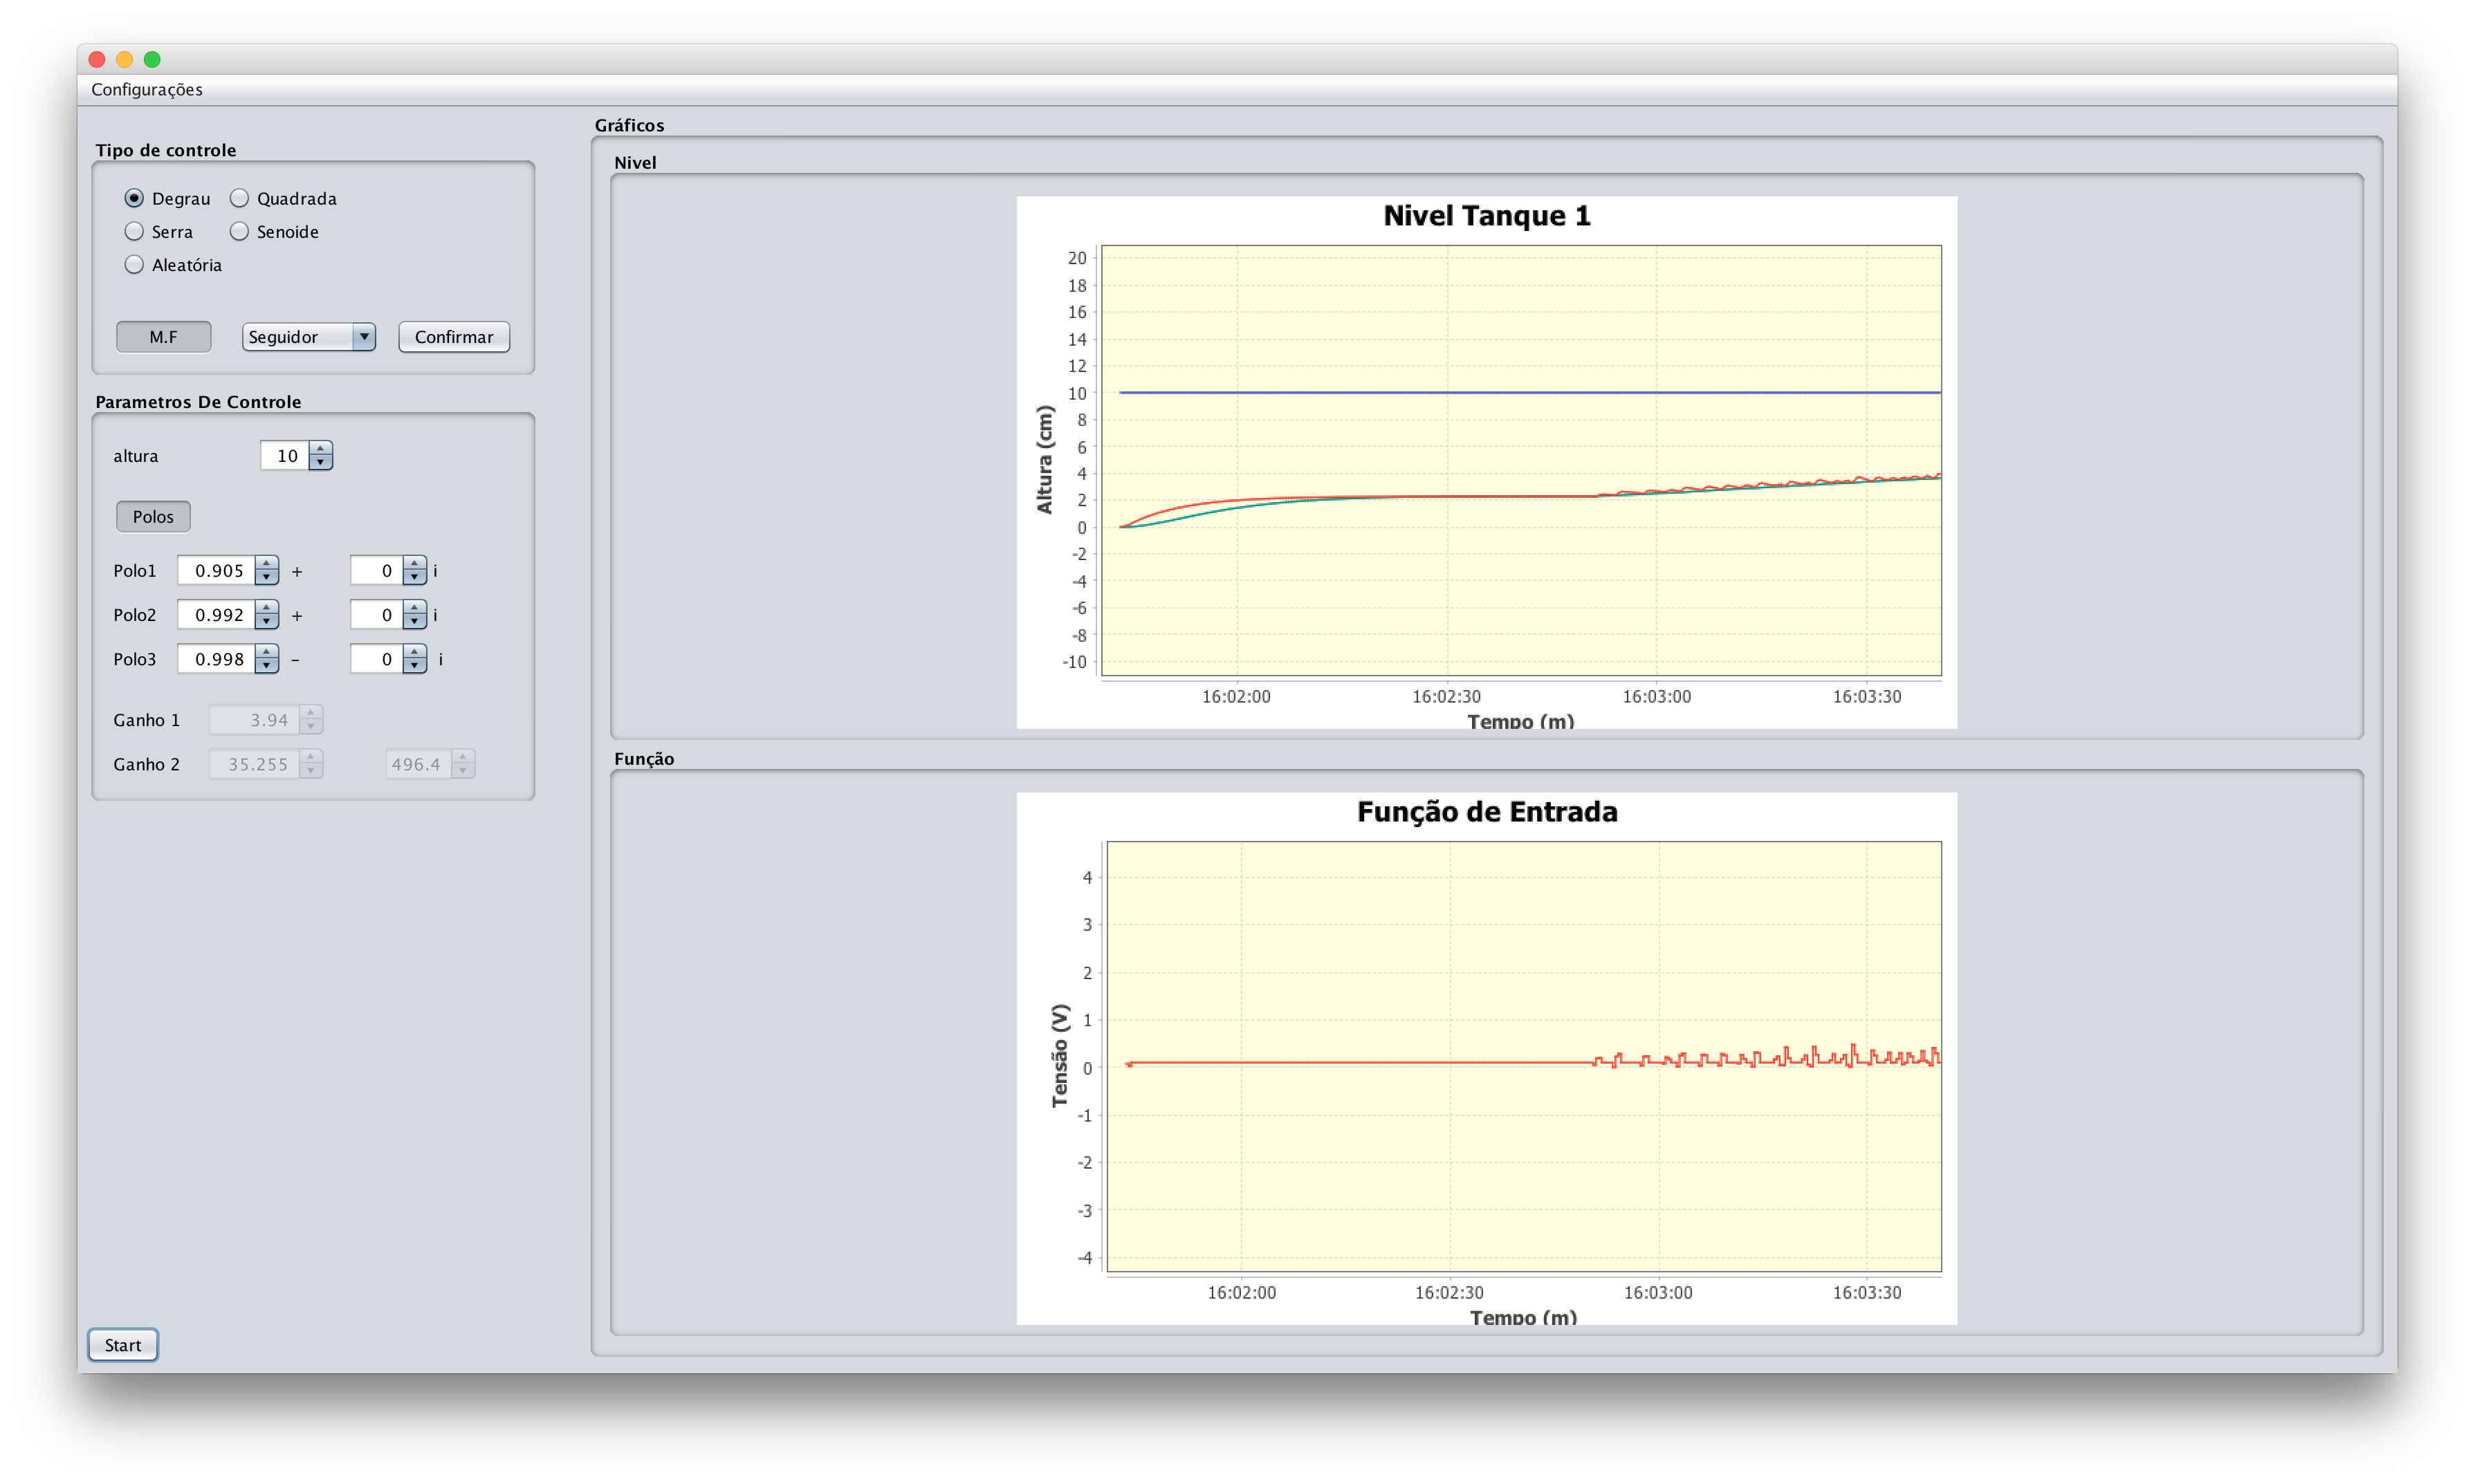
\includegraphics[scale=0.2]{Polos_0_905__0_992__0_998__2_}
\caption{Polos: 0.905; 0.992; 0.998}
\end{figure}

\begin{figure}[h!]
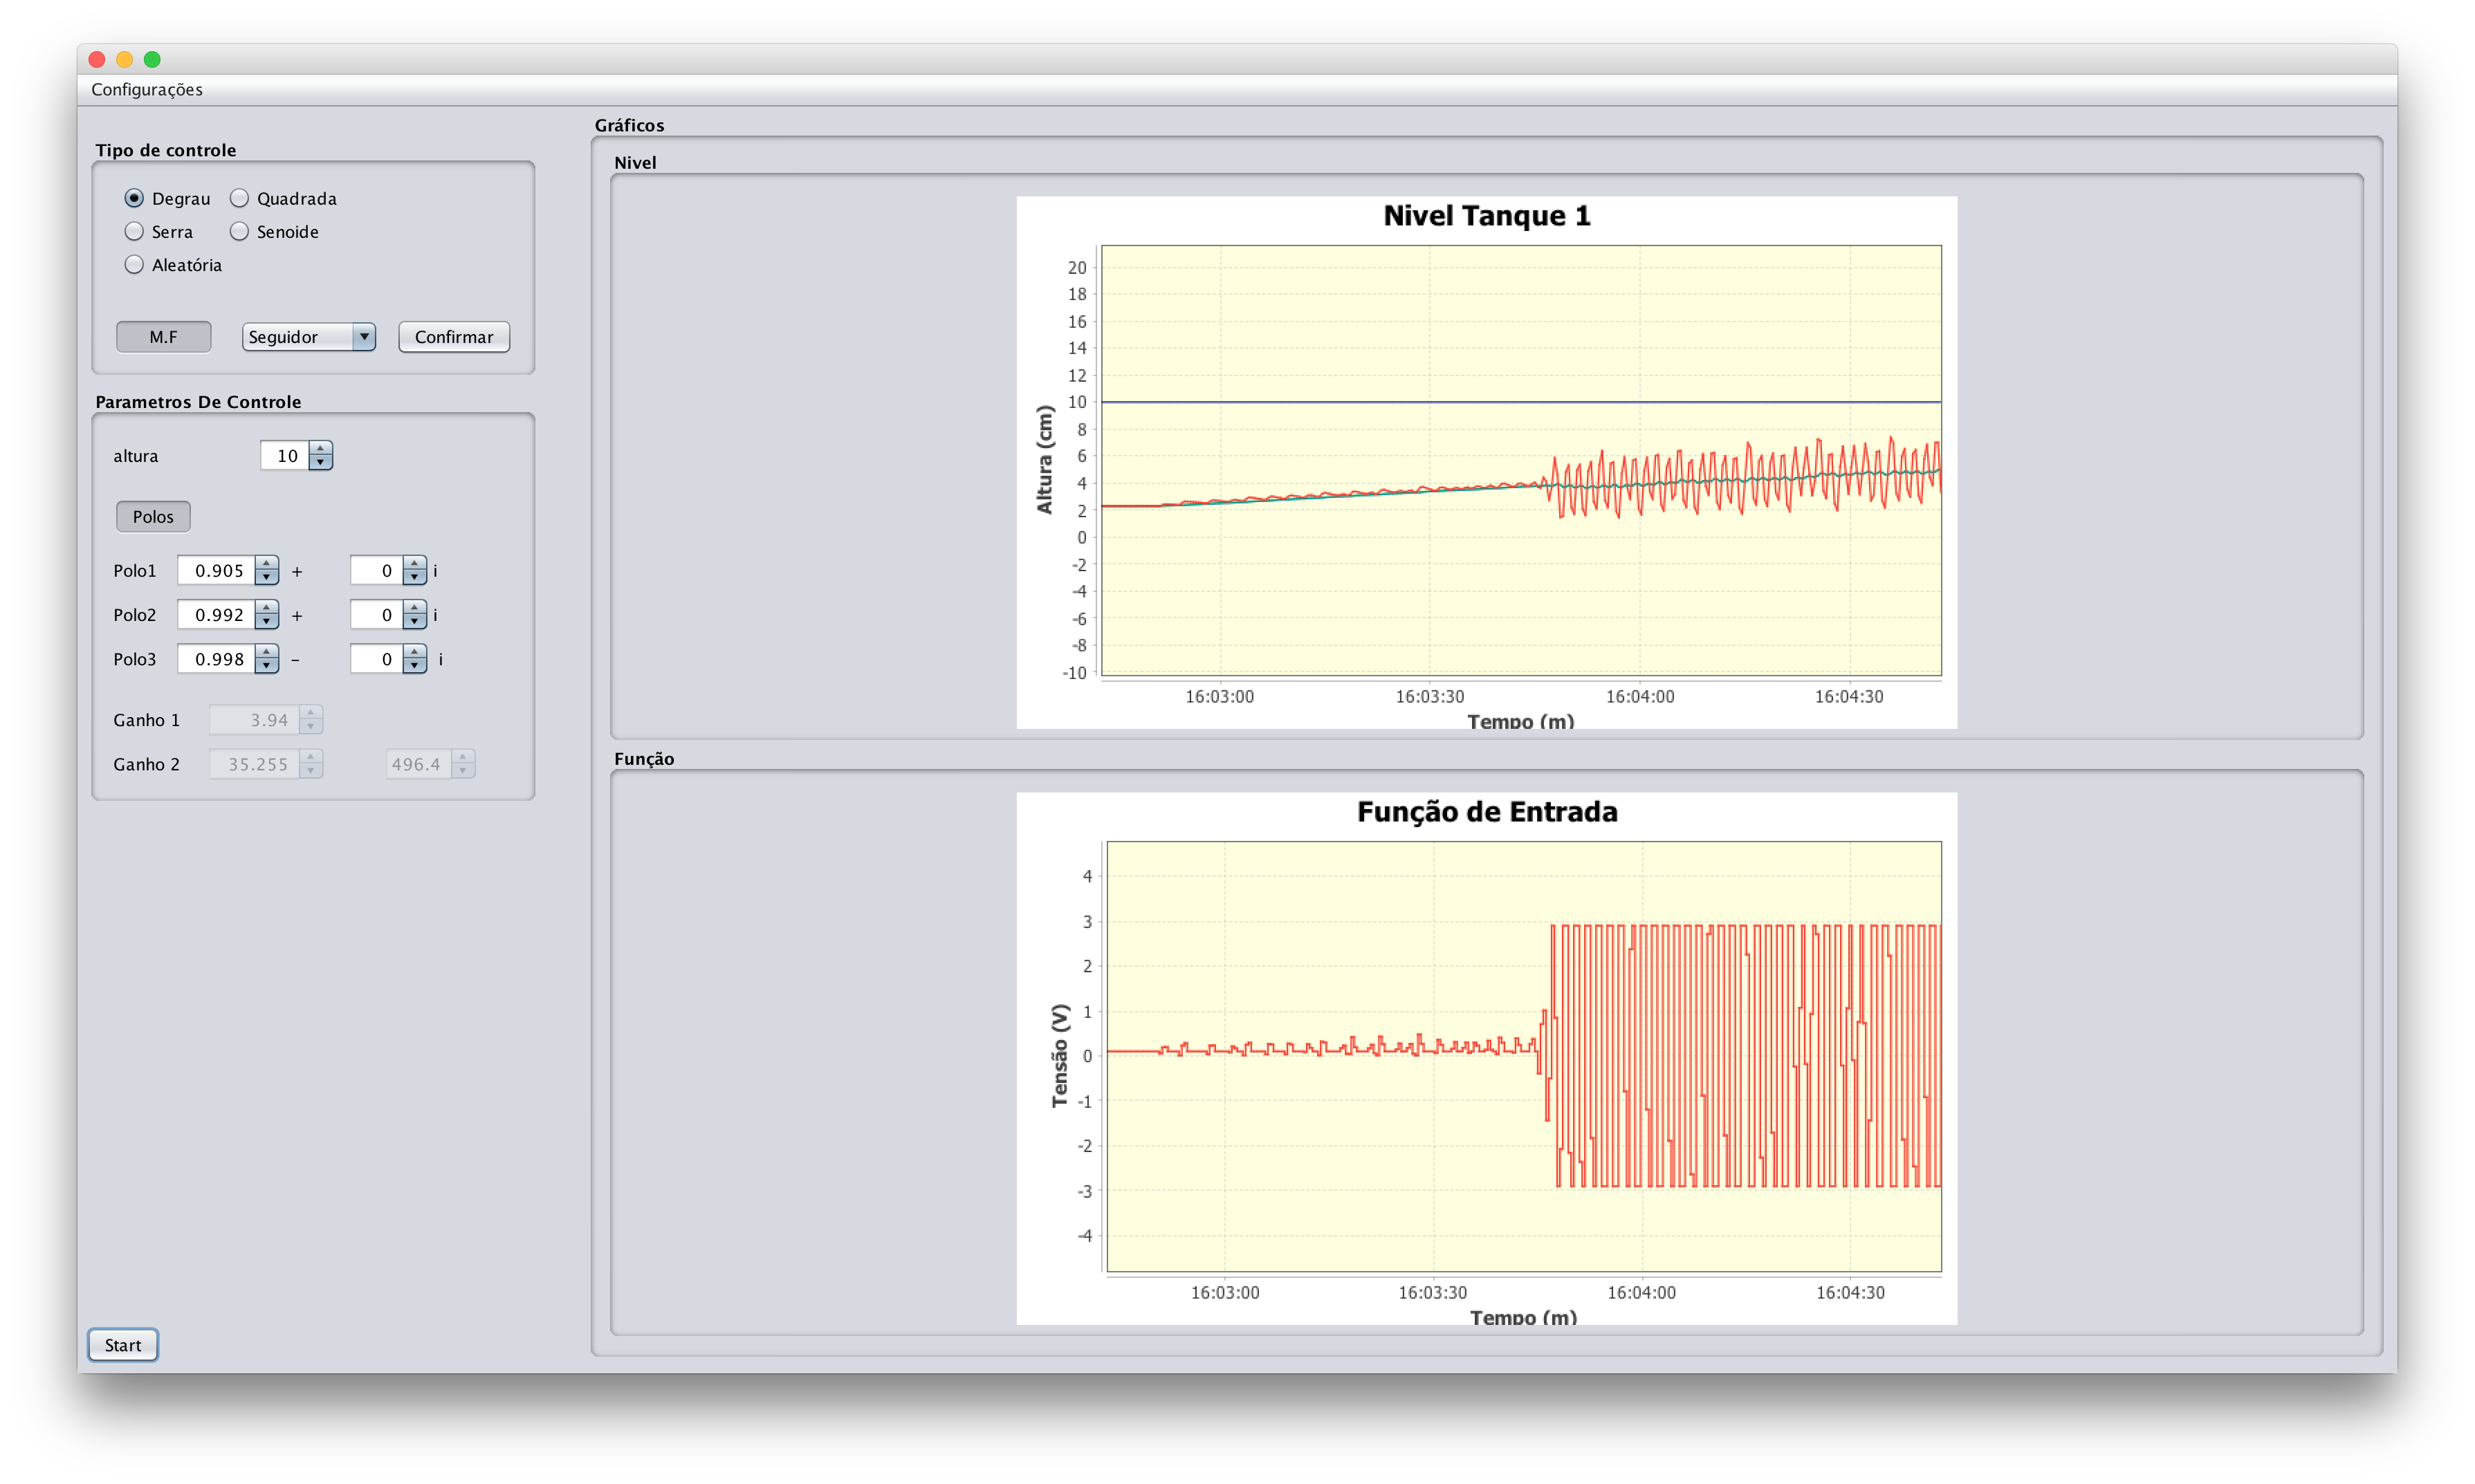
\includegraphics[scale=0.2]{Polos_0_905__0_992__0_998}
\caption{Segunda parte Polos: 0.905; 0.992; 0.998}
\end{figure}

\newpage

\thispagestyle{main}

\subsubsection{Polos em zero}

\hspace{4ex}Após os valores sugeridos no roteiro, foi testado o comportamento do sistema utilizando-se de polos em zero, como mostrado nas figuras 3, 4, 5 e 6 onde as respostas obtidas foram semelhantes a resposta do sistema com os polos sugeridos. Exceto no caso em que o polo 3 é zero, onda foi mostrada uma resposta também instável, porém com uma maior aproximação do valor do nivel do tanque 2 e do set point.

No caso em que dois dos polos eram zero, o sistema apresentou um resposta mais brusca, como mostrado na figura 6.

\begin{figure}[h!]
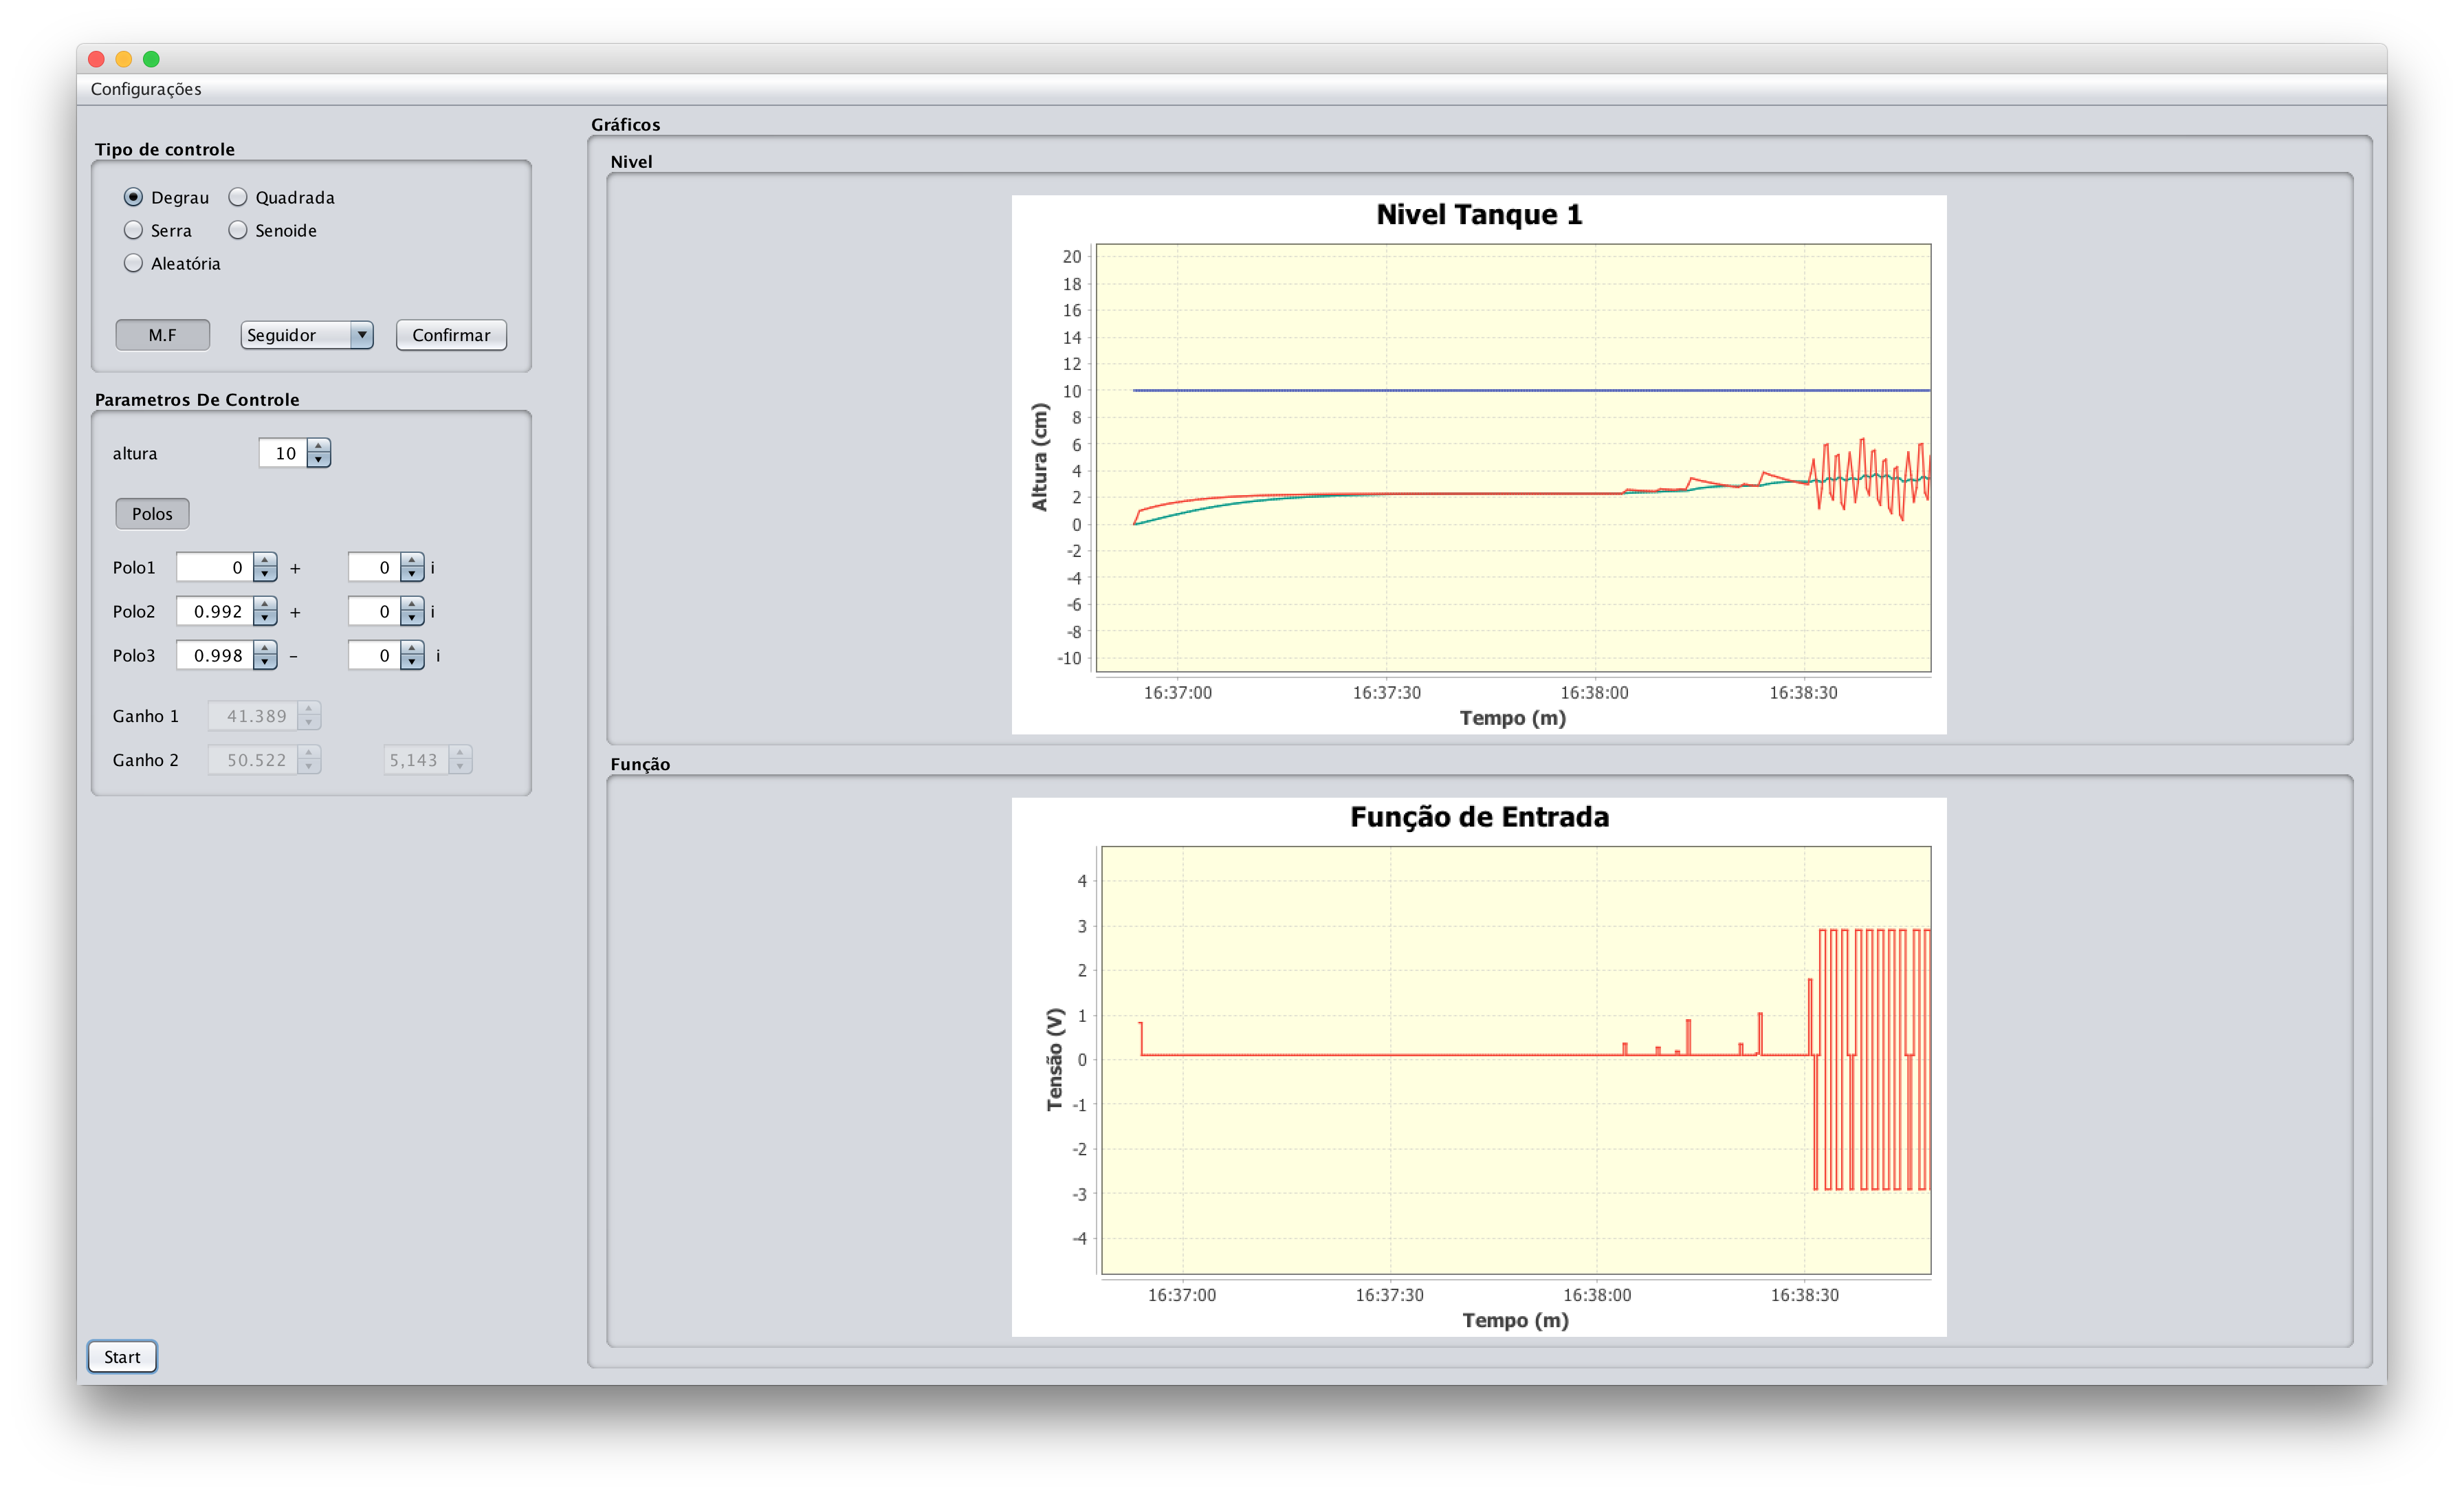
\includegraphics[scale=0.2]{Polos_0__0_992__0_998}
\caption{Polos: 0; 0.992; 0.998}
\end{figure}

\begin{figure}[h!]
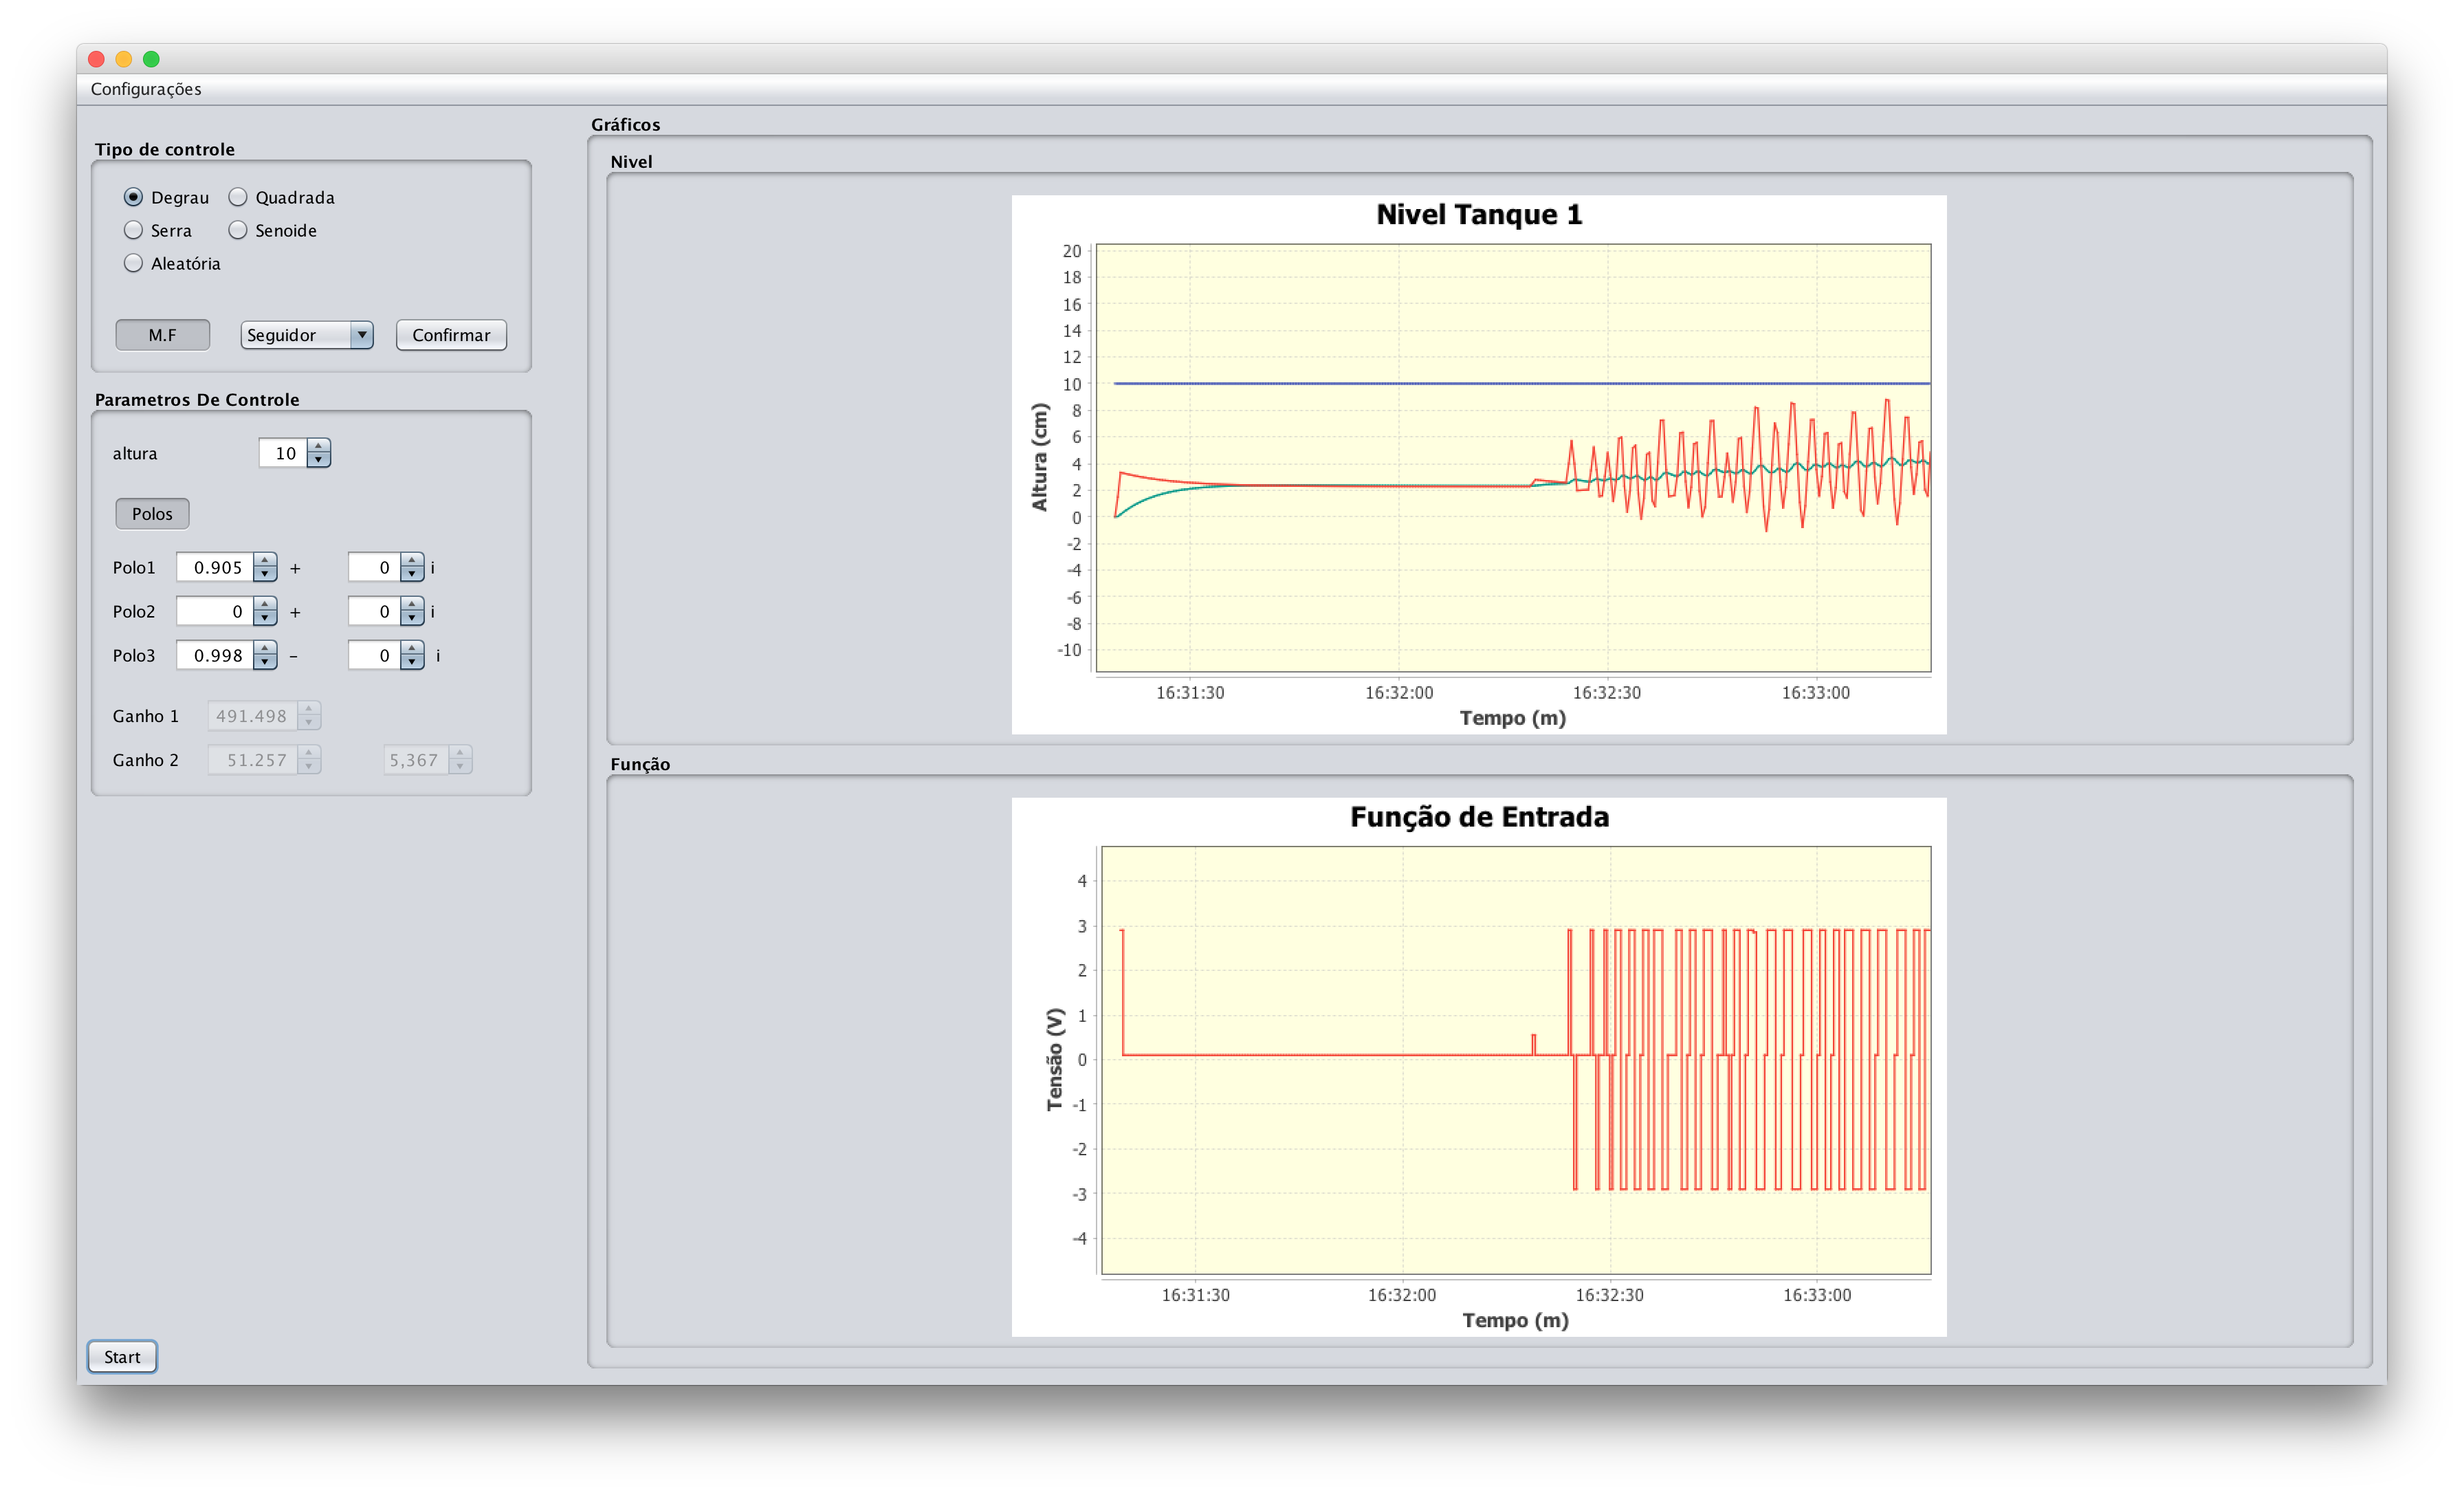
\includegraphics[scale=0.2]{Polo_0_905__0__0_998__2_}
\caption{Polos: 0.905; 0; 0.998}
\end{figure}

\newpage

\thispagestyle{main}

\begin{figure}[h!]
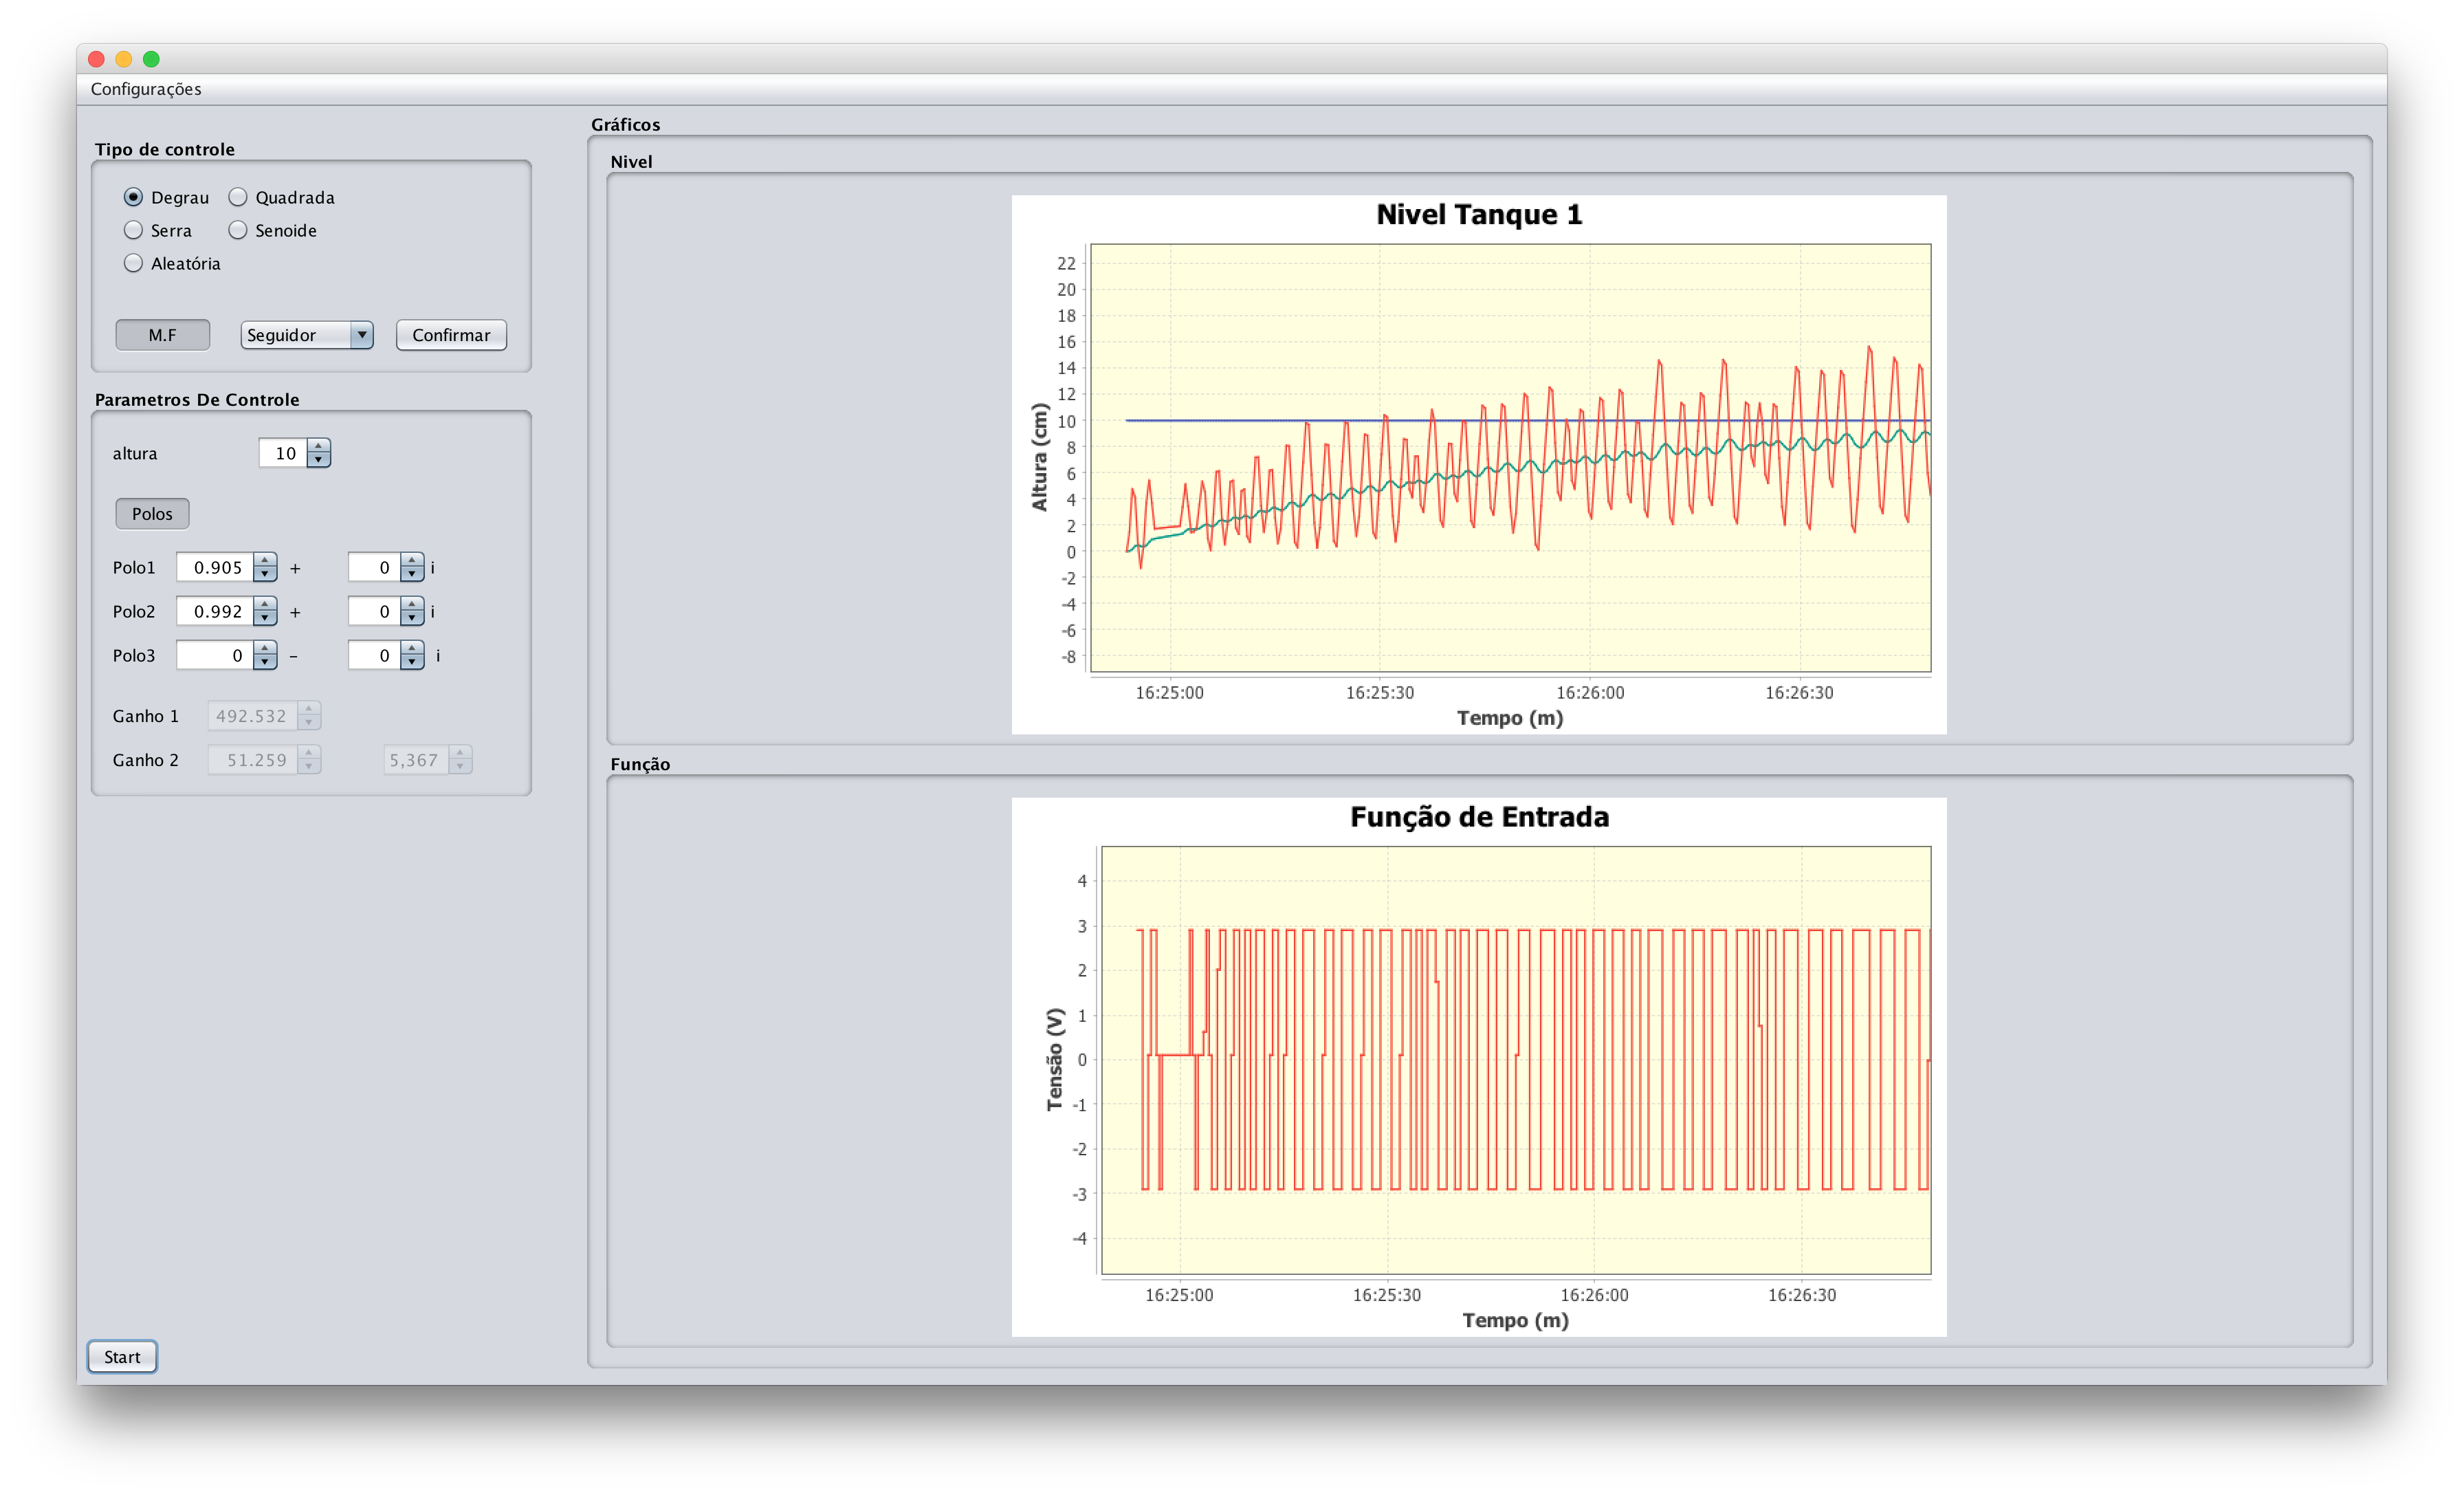
\includegraphics[scale=0.2]{Polos_0_905__0_992__0__2_}
\caption{Polos: 0.905; 0.992; 0}
\end{figure}

\begin{figure}[h!]
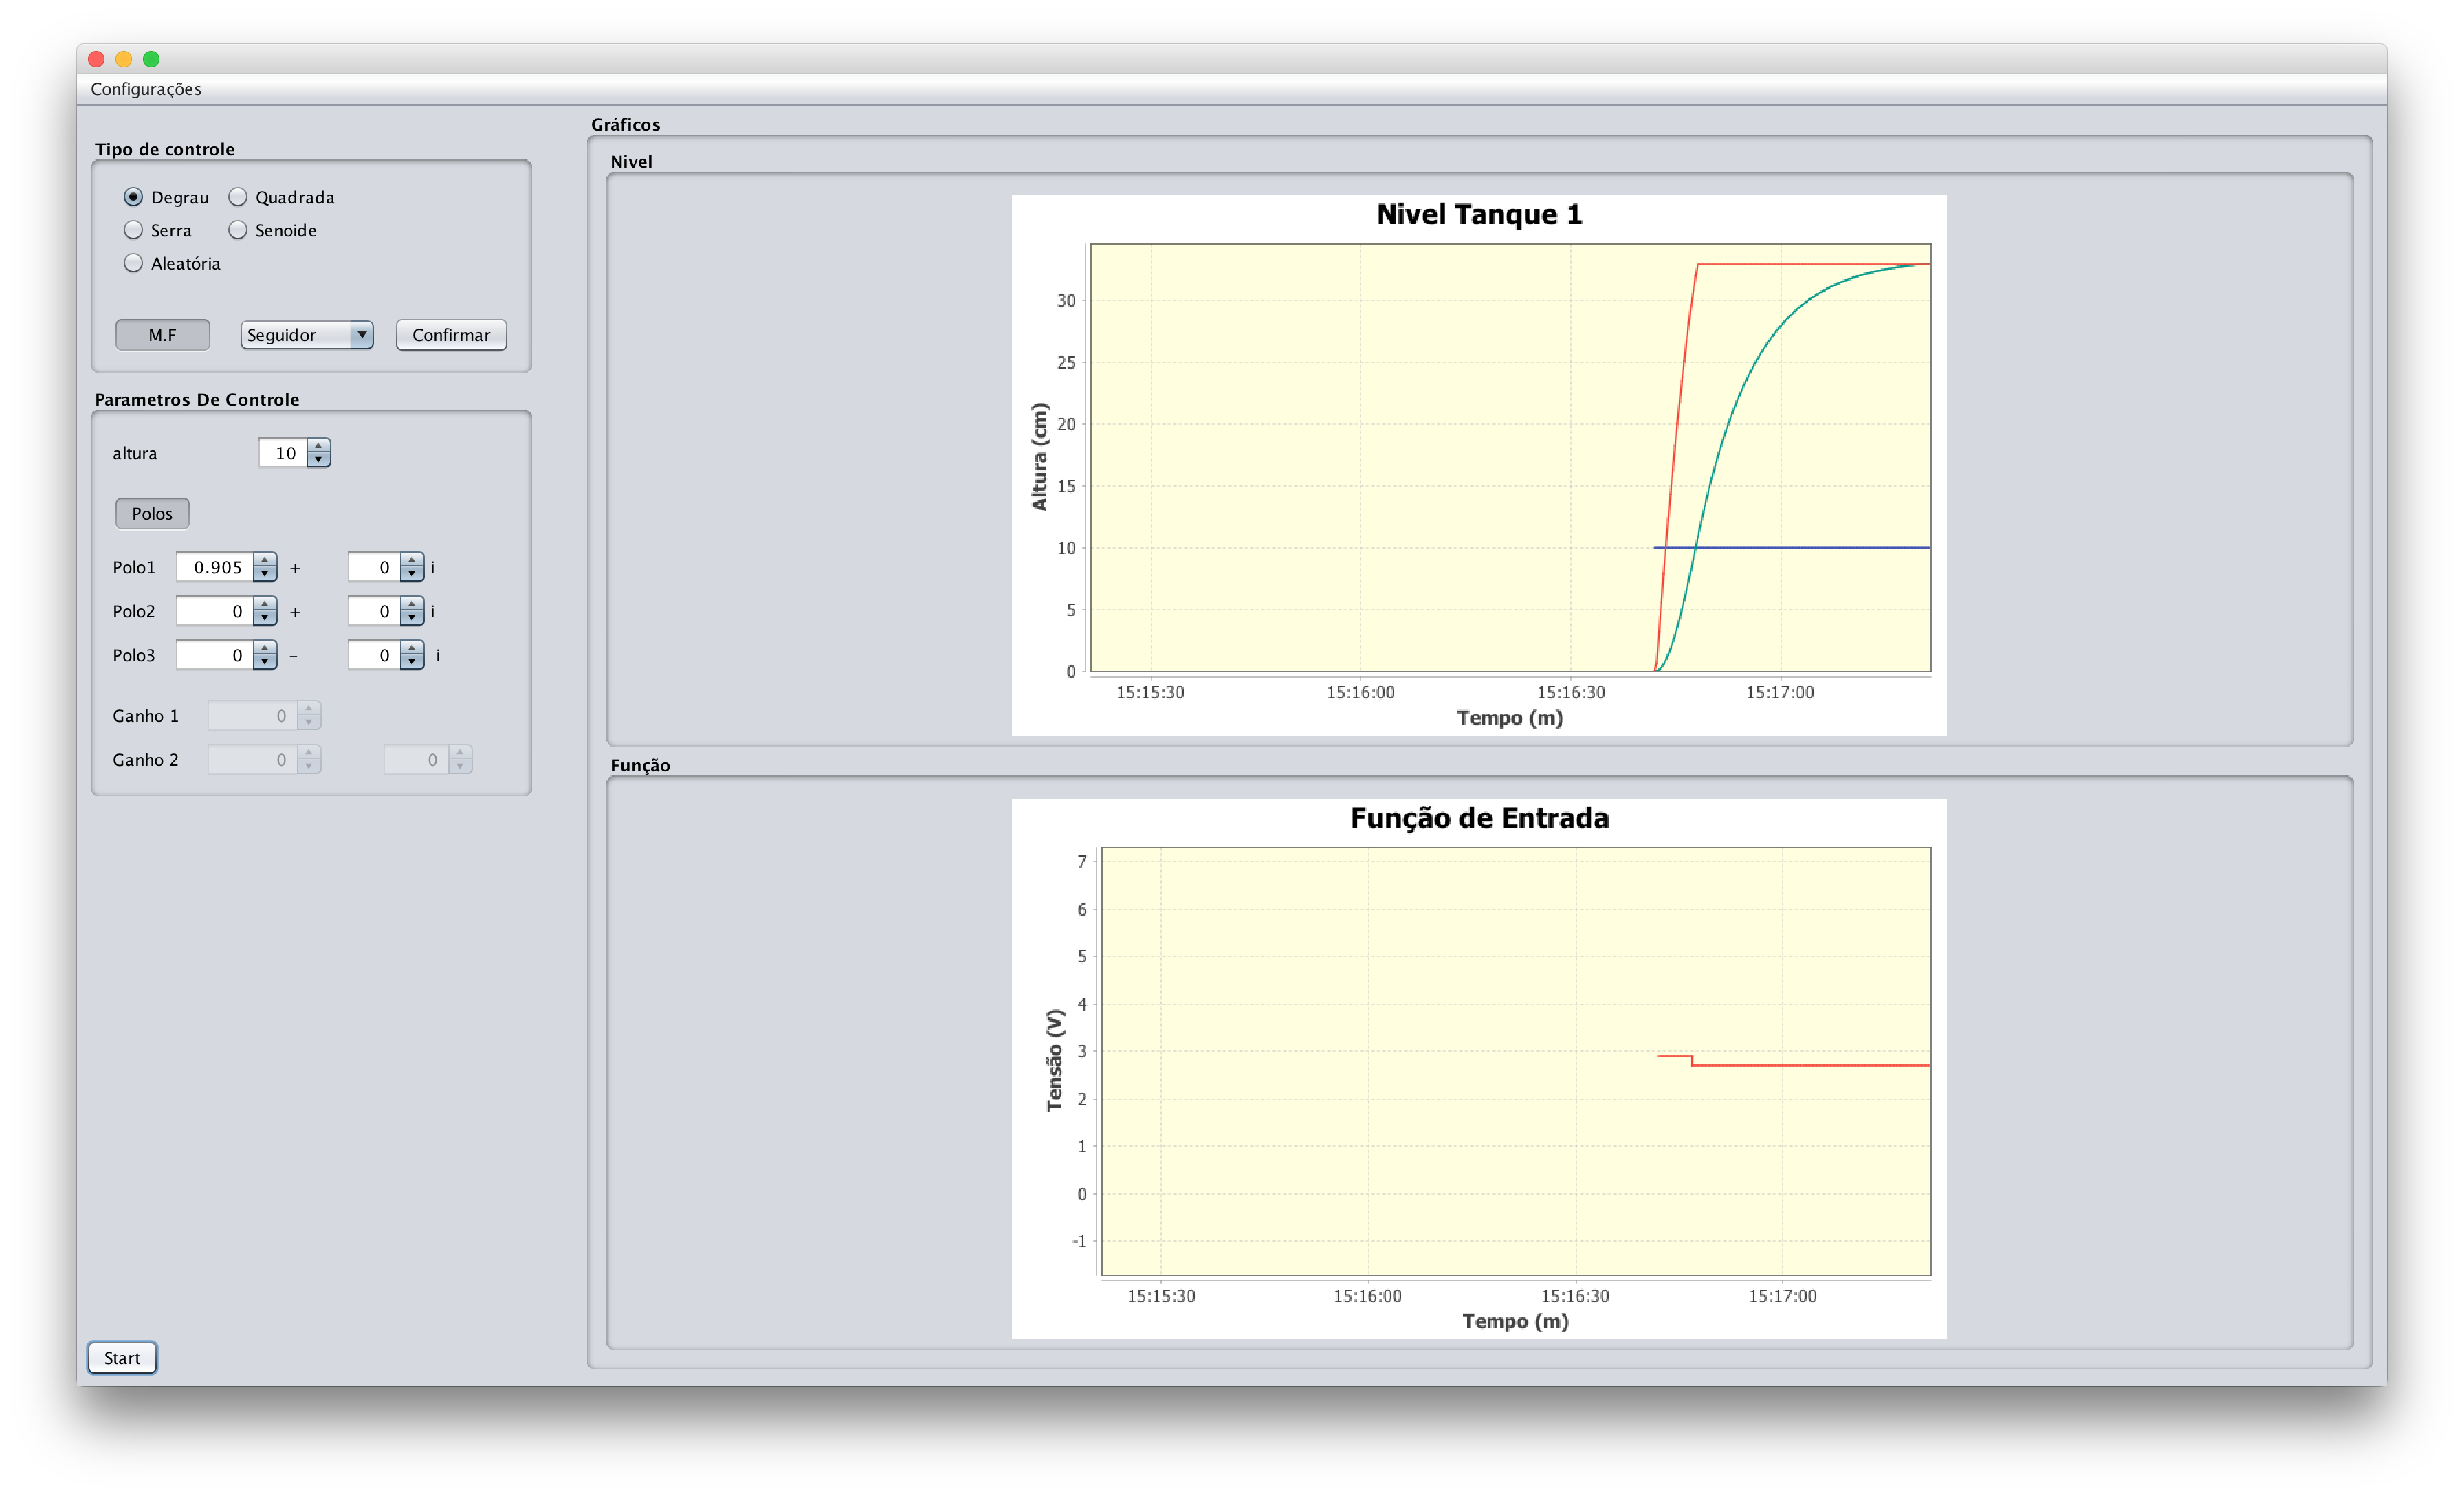
\includegraphics[scale=0.2]{Polos_0_905__0__0}
\caption{Polos: 0.905; 0; 0}
\end{figure}

\newpage

\thispagestyle{main}

\subsubsection{Valores acima de 1}

\hspace{4ex}Foram testados também, valores acima de 1 para os polos, na qual a resposta do sistema esta mostrado nas Figuras 7, 8 e 9. Nestas figuras, podemos ver o comportamento semelhante ao sistema com polos em zero, com excessão da figura 9, na qual mostra o polo 3 em 1.2. Neste caso, a resposta se assemelha ao comportamento do sistema com os polos sugeridos no roteiro do experimento. 
Além deste valor, foram testados outros valores para o polo 3, onde, em todos os testes, foi notado pouca influência na resposta do sistema.

\begin{figure}[h!]
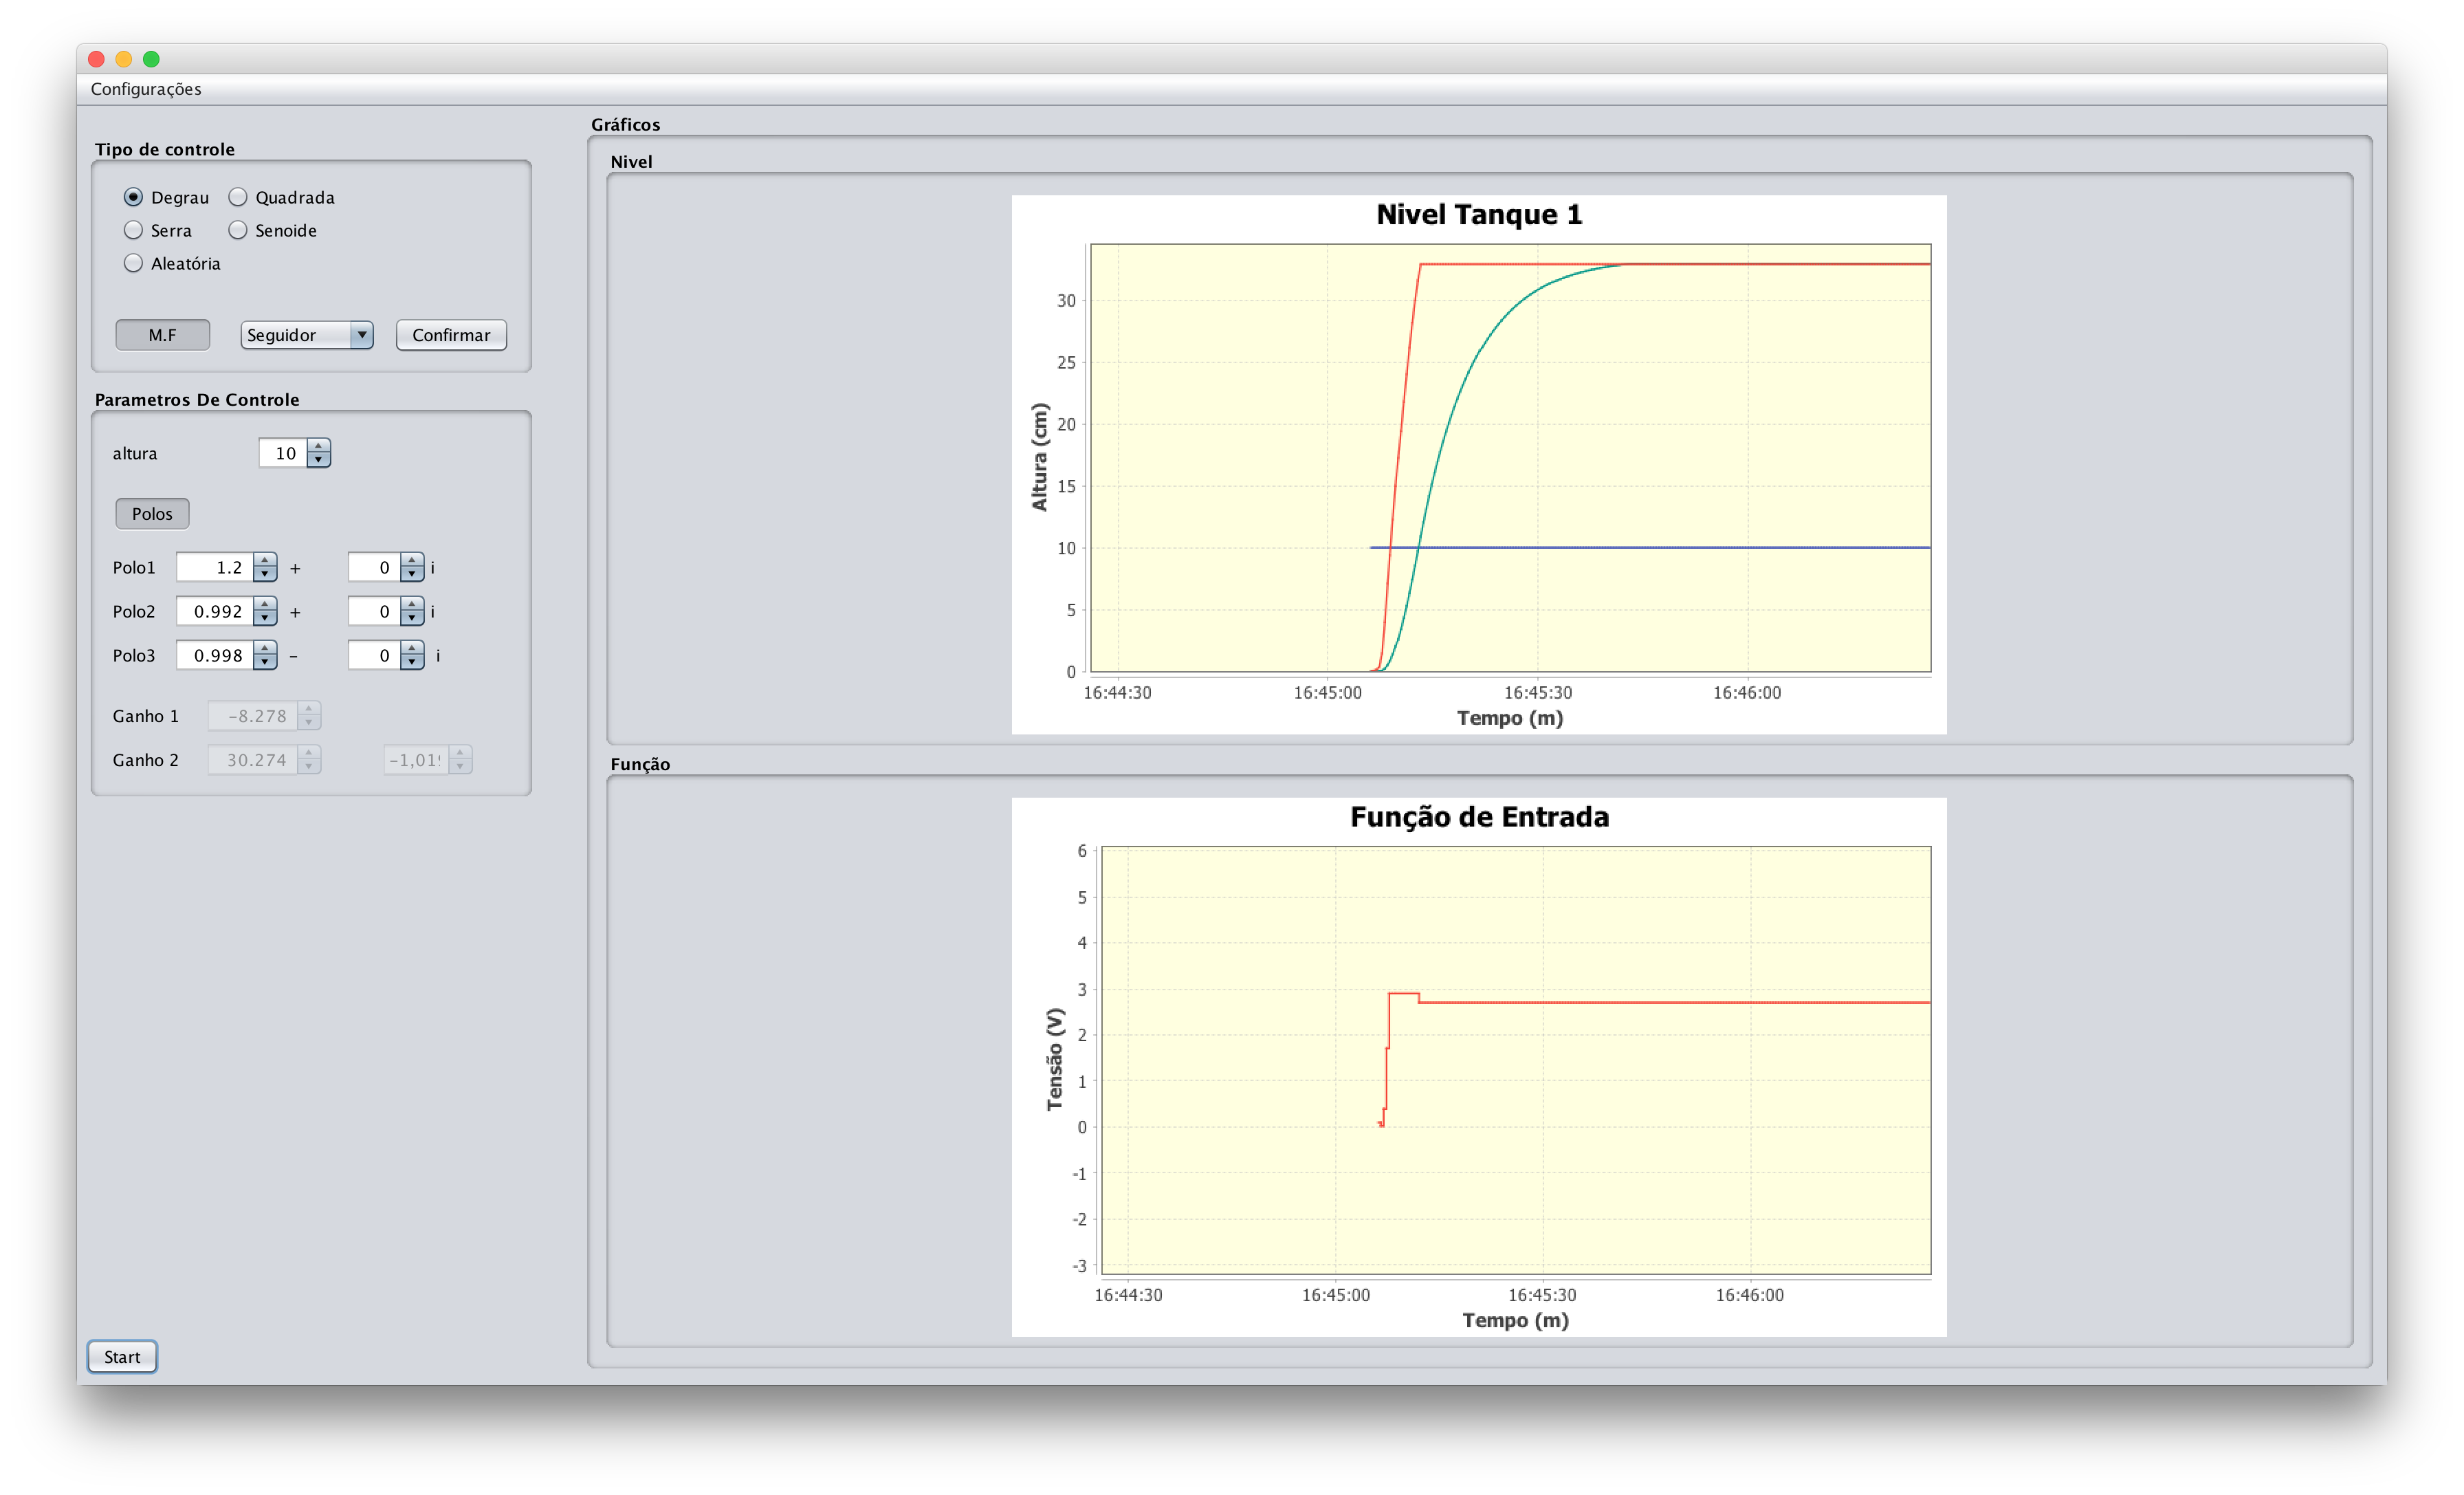
\includegraphics[scale=0.2]{Polos_1_2__0_992__0_998}
\caption{Polos: 1.2; 0.992; 0.998}
\end{figure}

\begin{figure}[h!]
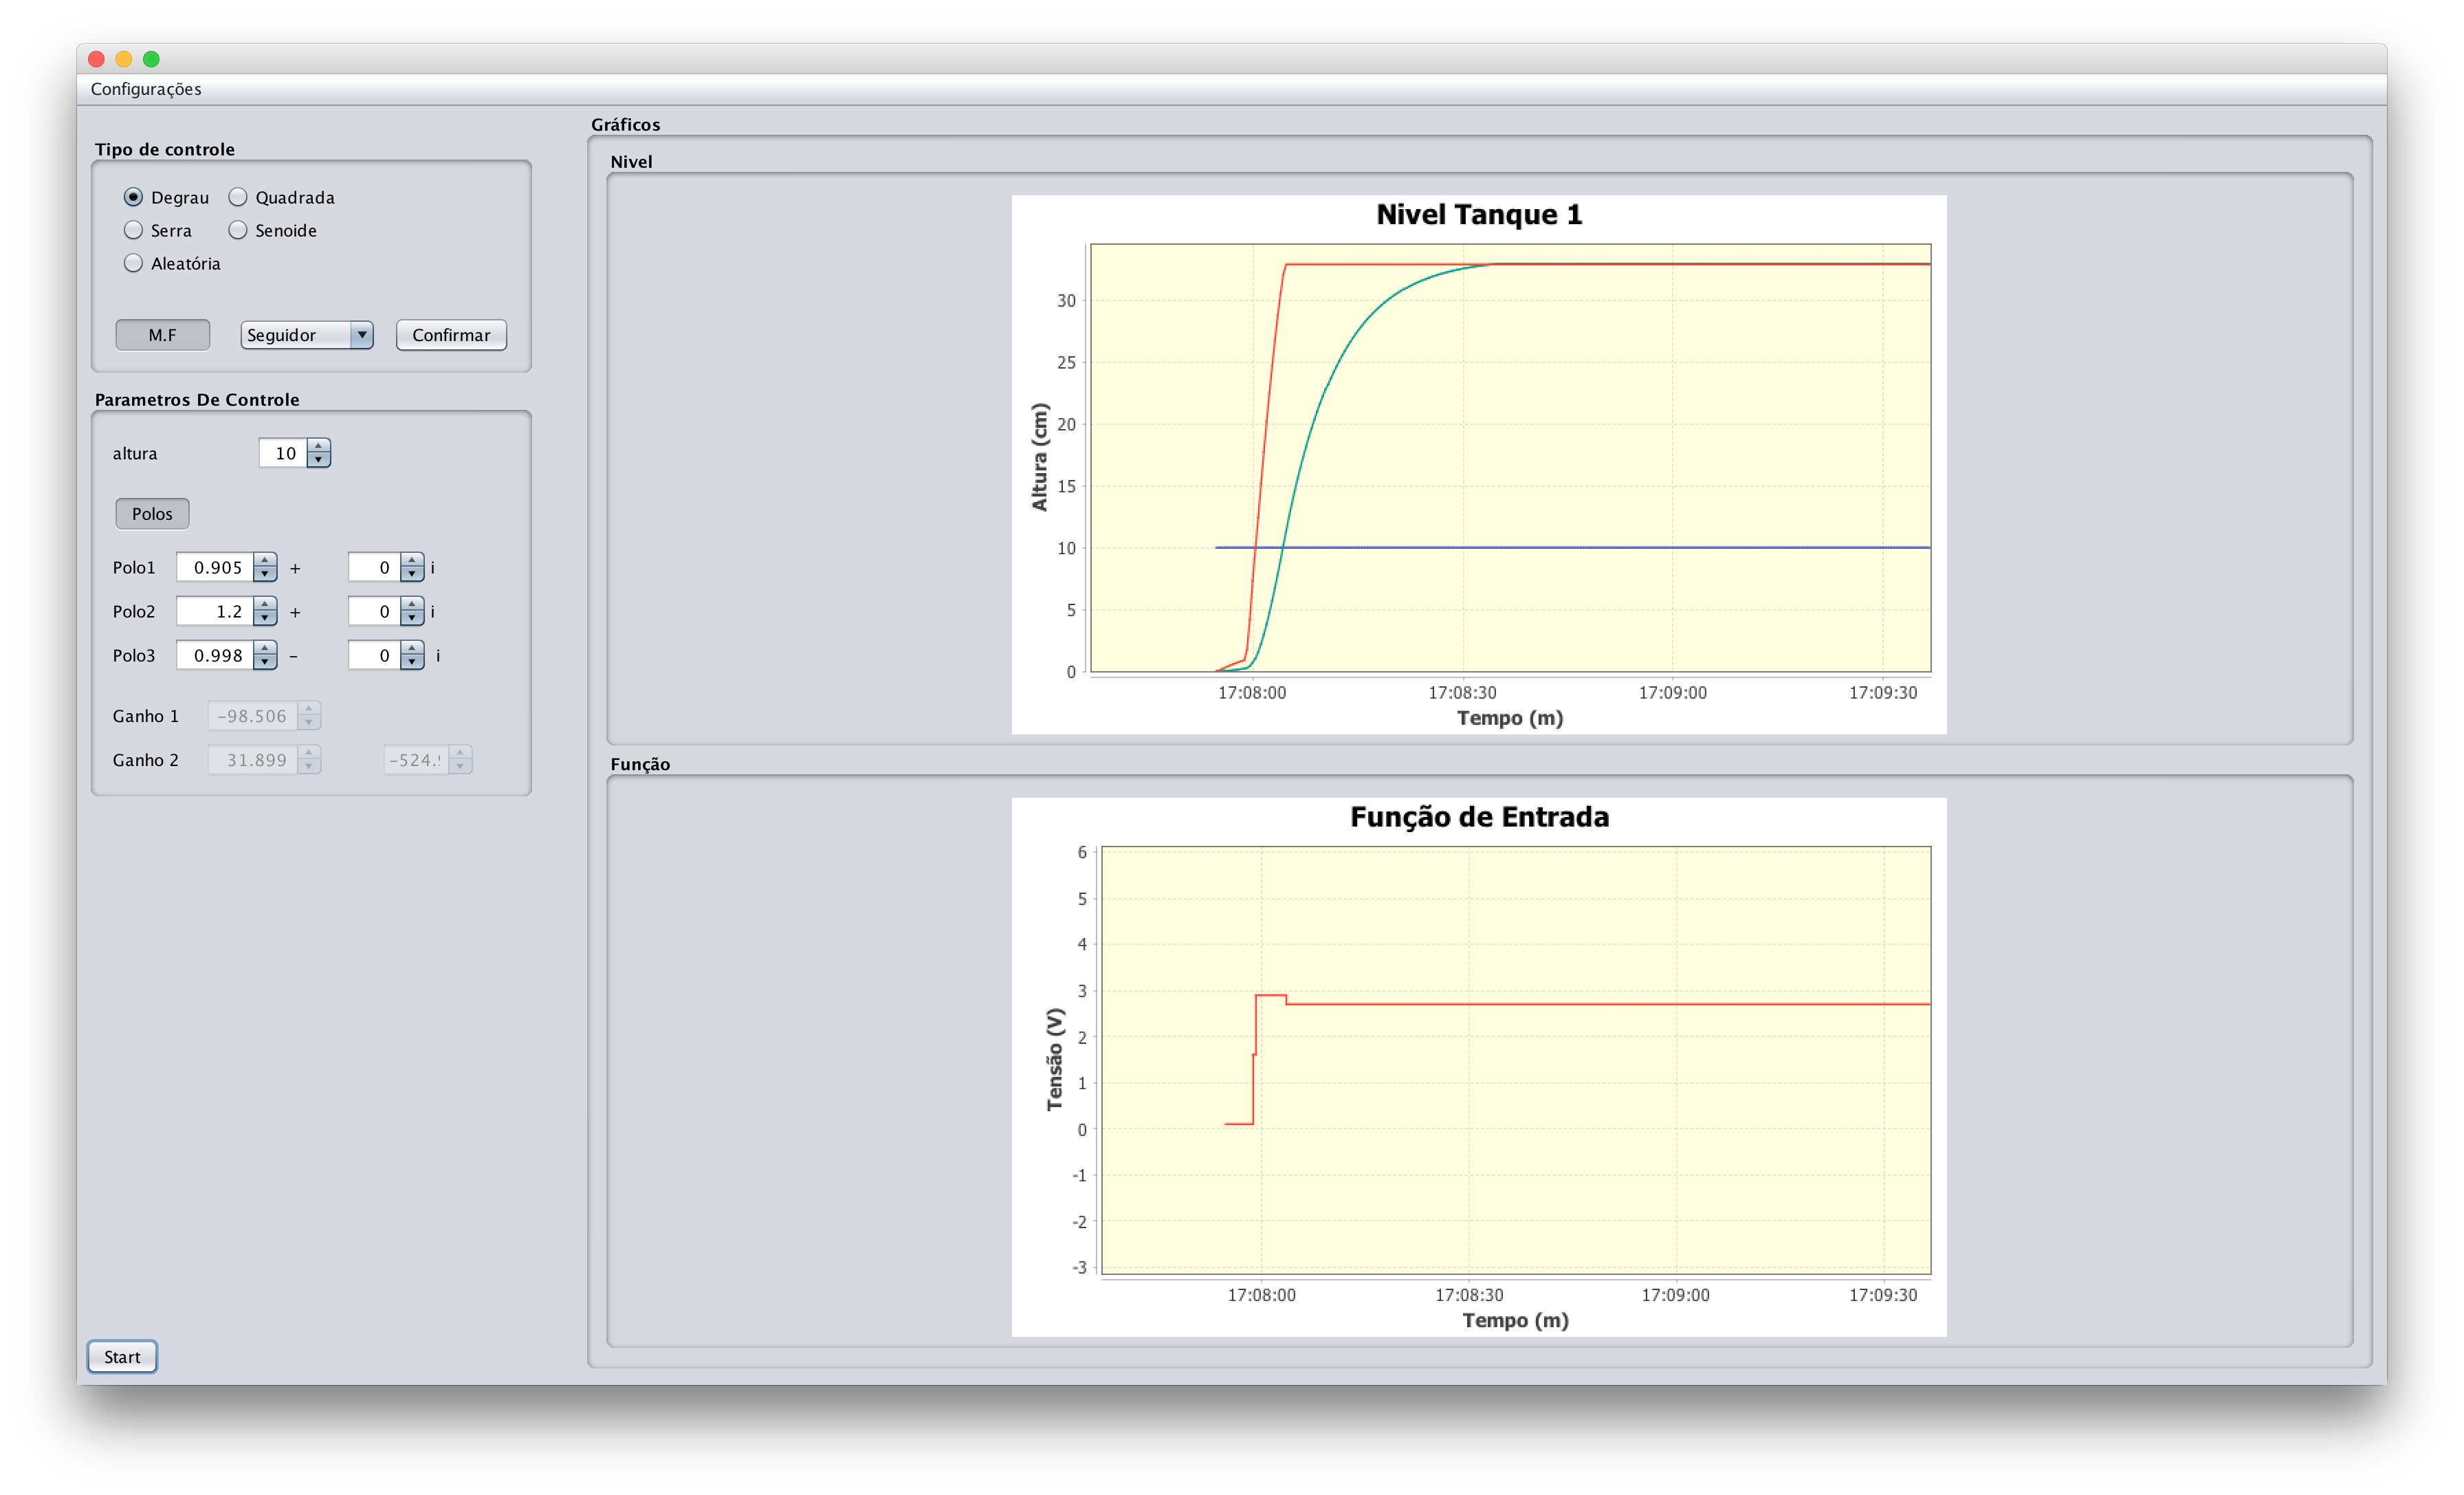
\includegraphics[scale=0.2]{Polos_0_905__1_2__0_998}
\caption{Polos: 0.905; 1.2; 0.998}
\end{figure}

\newpage

\thispagestyle{main}

\begin{figure}[h!]
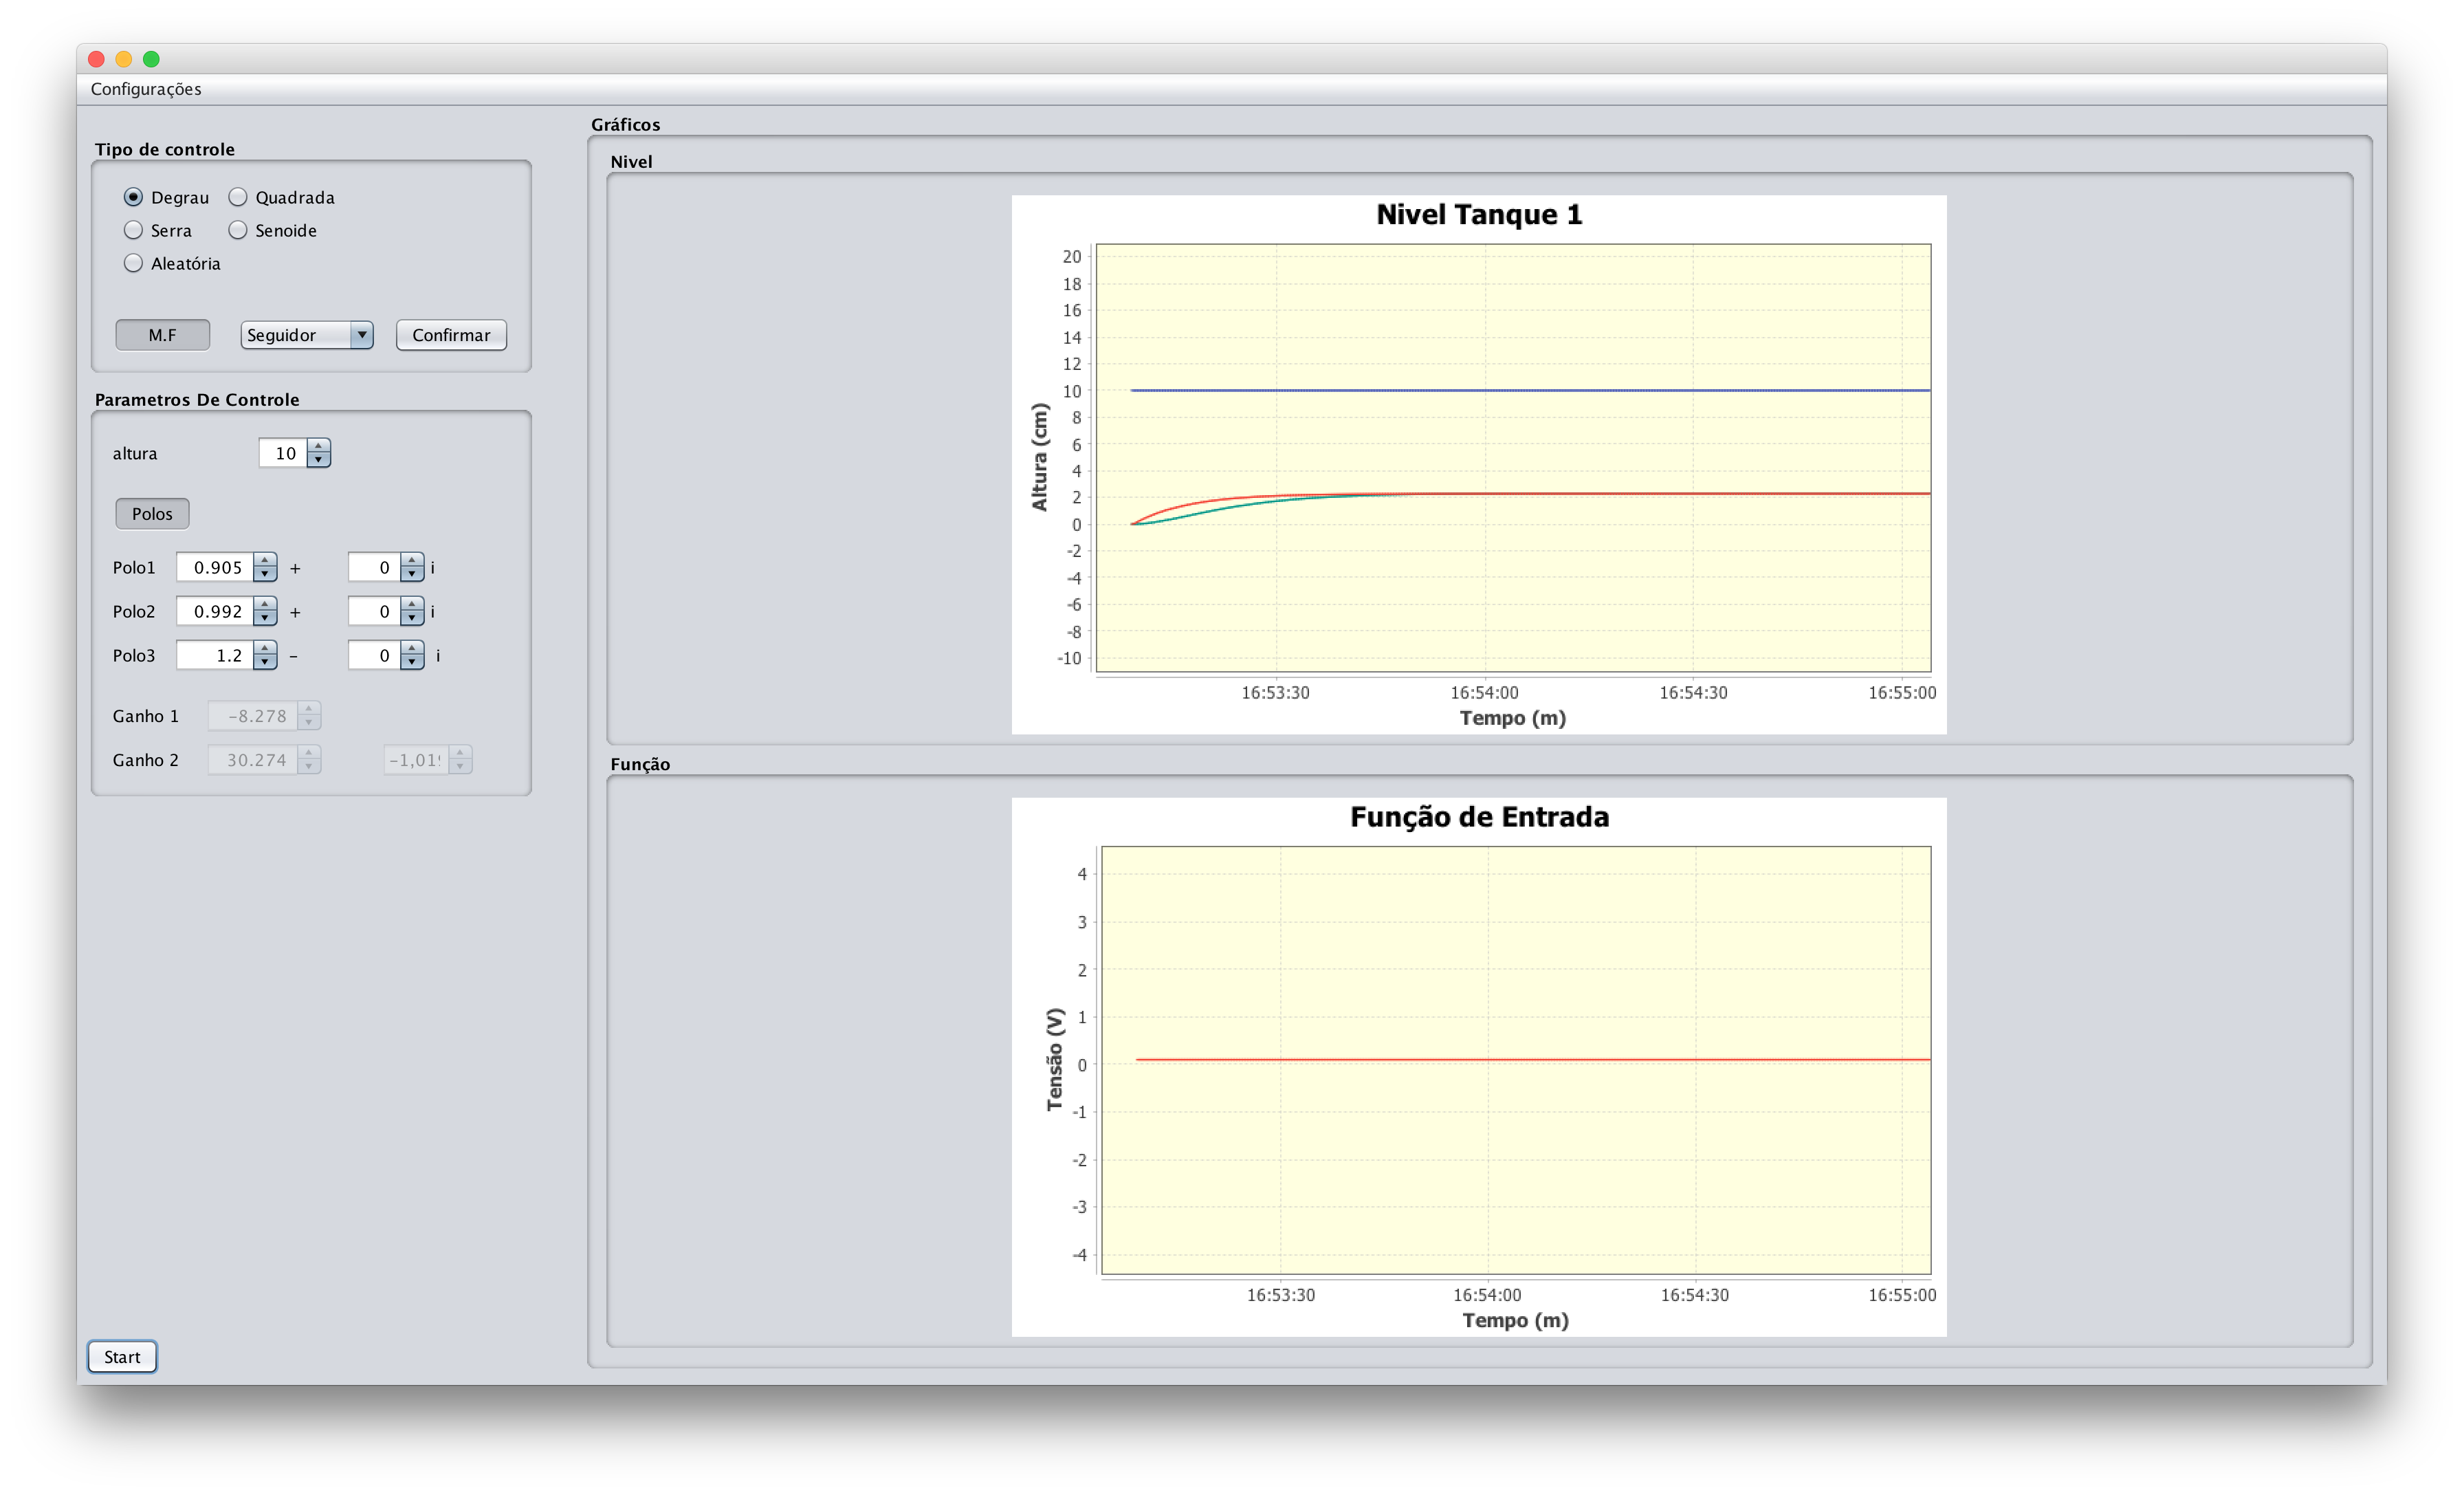
\includegraphics[scale=0.2]{Polos_0_905__0_992__1_2}
\caption{Polos: 0.905; 0.992; 1.2}
\end{figure}

\newpage

\thispagestyle{main}

\subsubsection{Valor imaginario diferente de zero}

\hspace{4ex}Nas Figuras 10, 11, 12 e 13 são mostrados os testes realizados com polos com parte imaginária diferente de zero, onde a melhor das respostas foi o sistema com polo com parte imaginária igual a 0.03 (Figura 10).
Para os outros valores testados, pode-se notar uma instabilidade do sistema ao utilizar a parte imaginária dos polos em torno de 0.1. Além disso, foi notado mais uma vez pouca influência do polo 3 sobre o comportamento do sistema. 

\begin{figure}[h!]
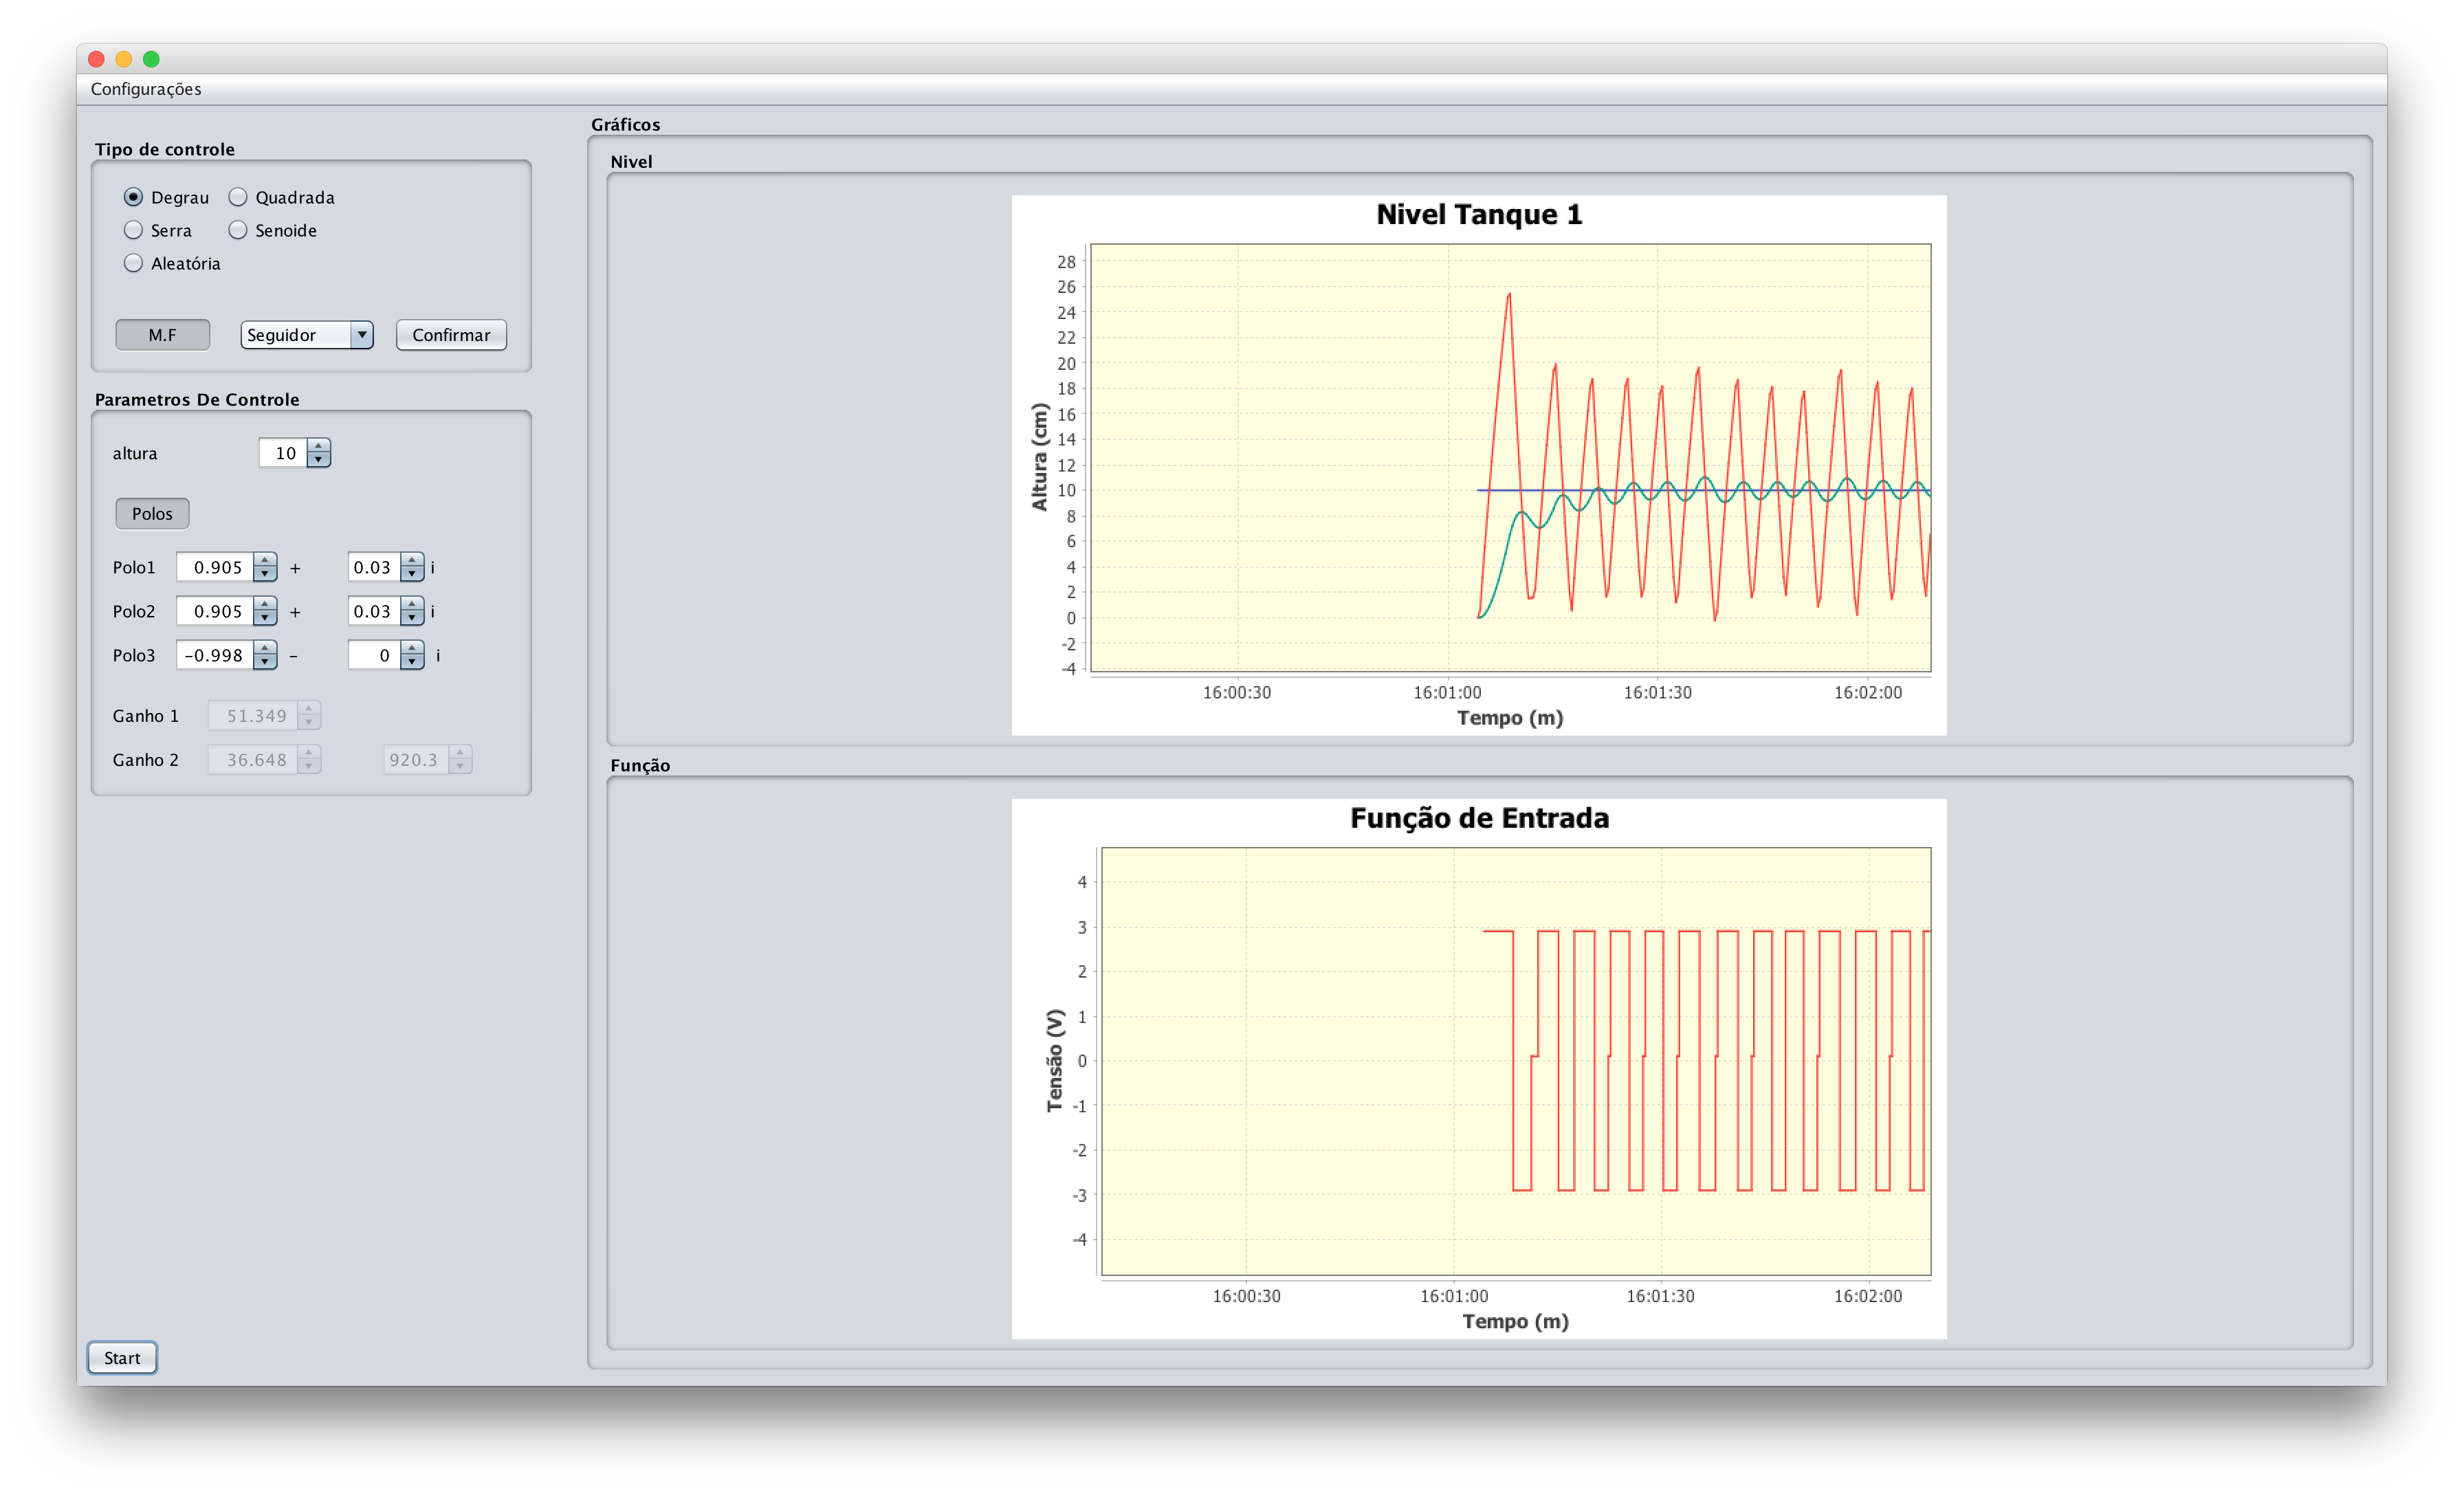
\includegraphics[scale=0.2]{Polos_0_905_i0_03__-0_998}
\caption{Polos: 0.905 + i0.03; 0.905 + i0.03; -0.998}
\end{figure}

\begin{figure}[h!]
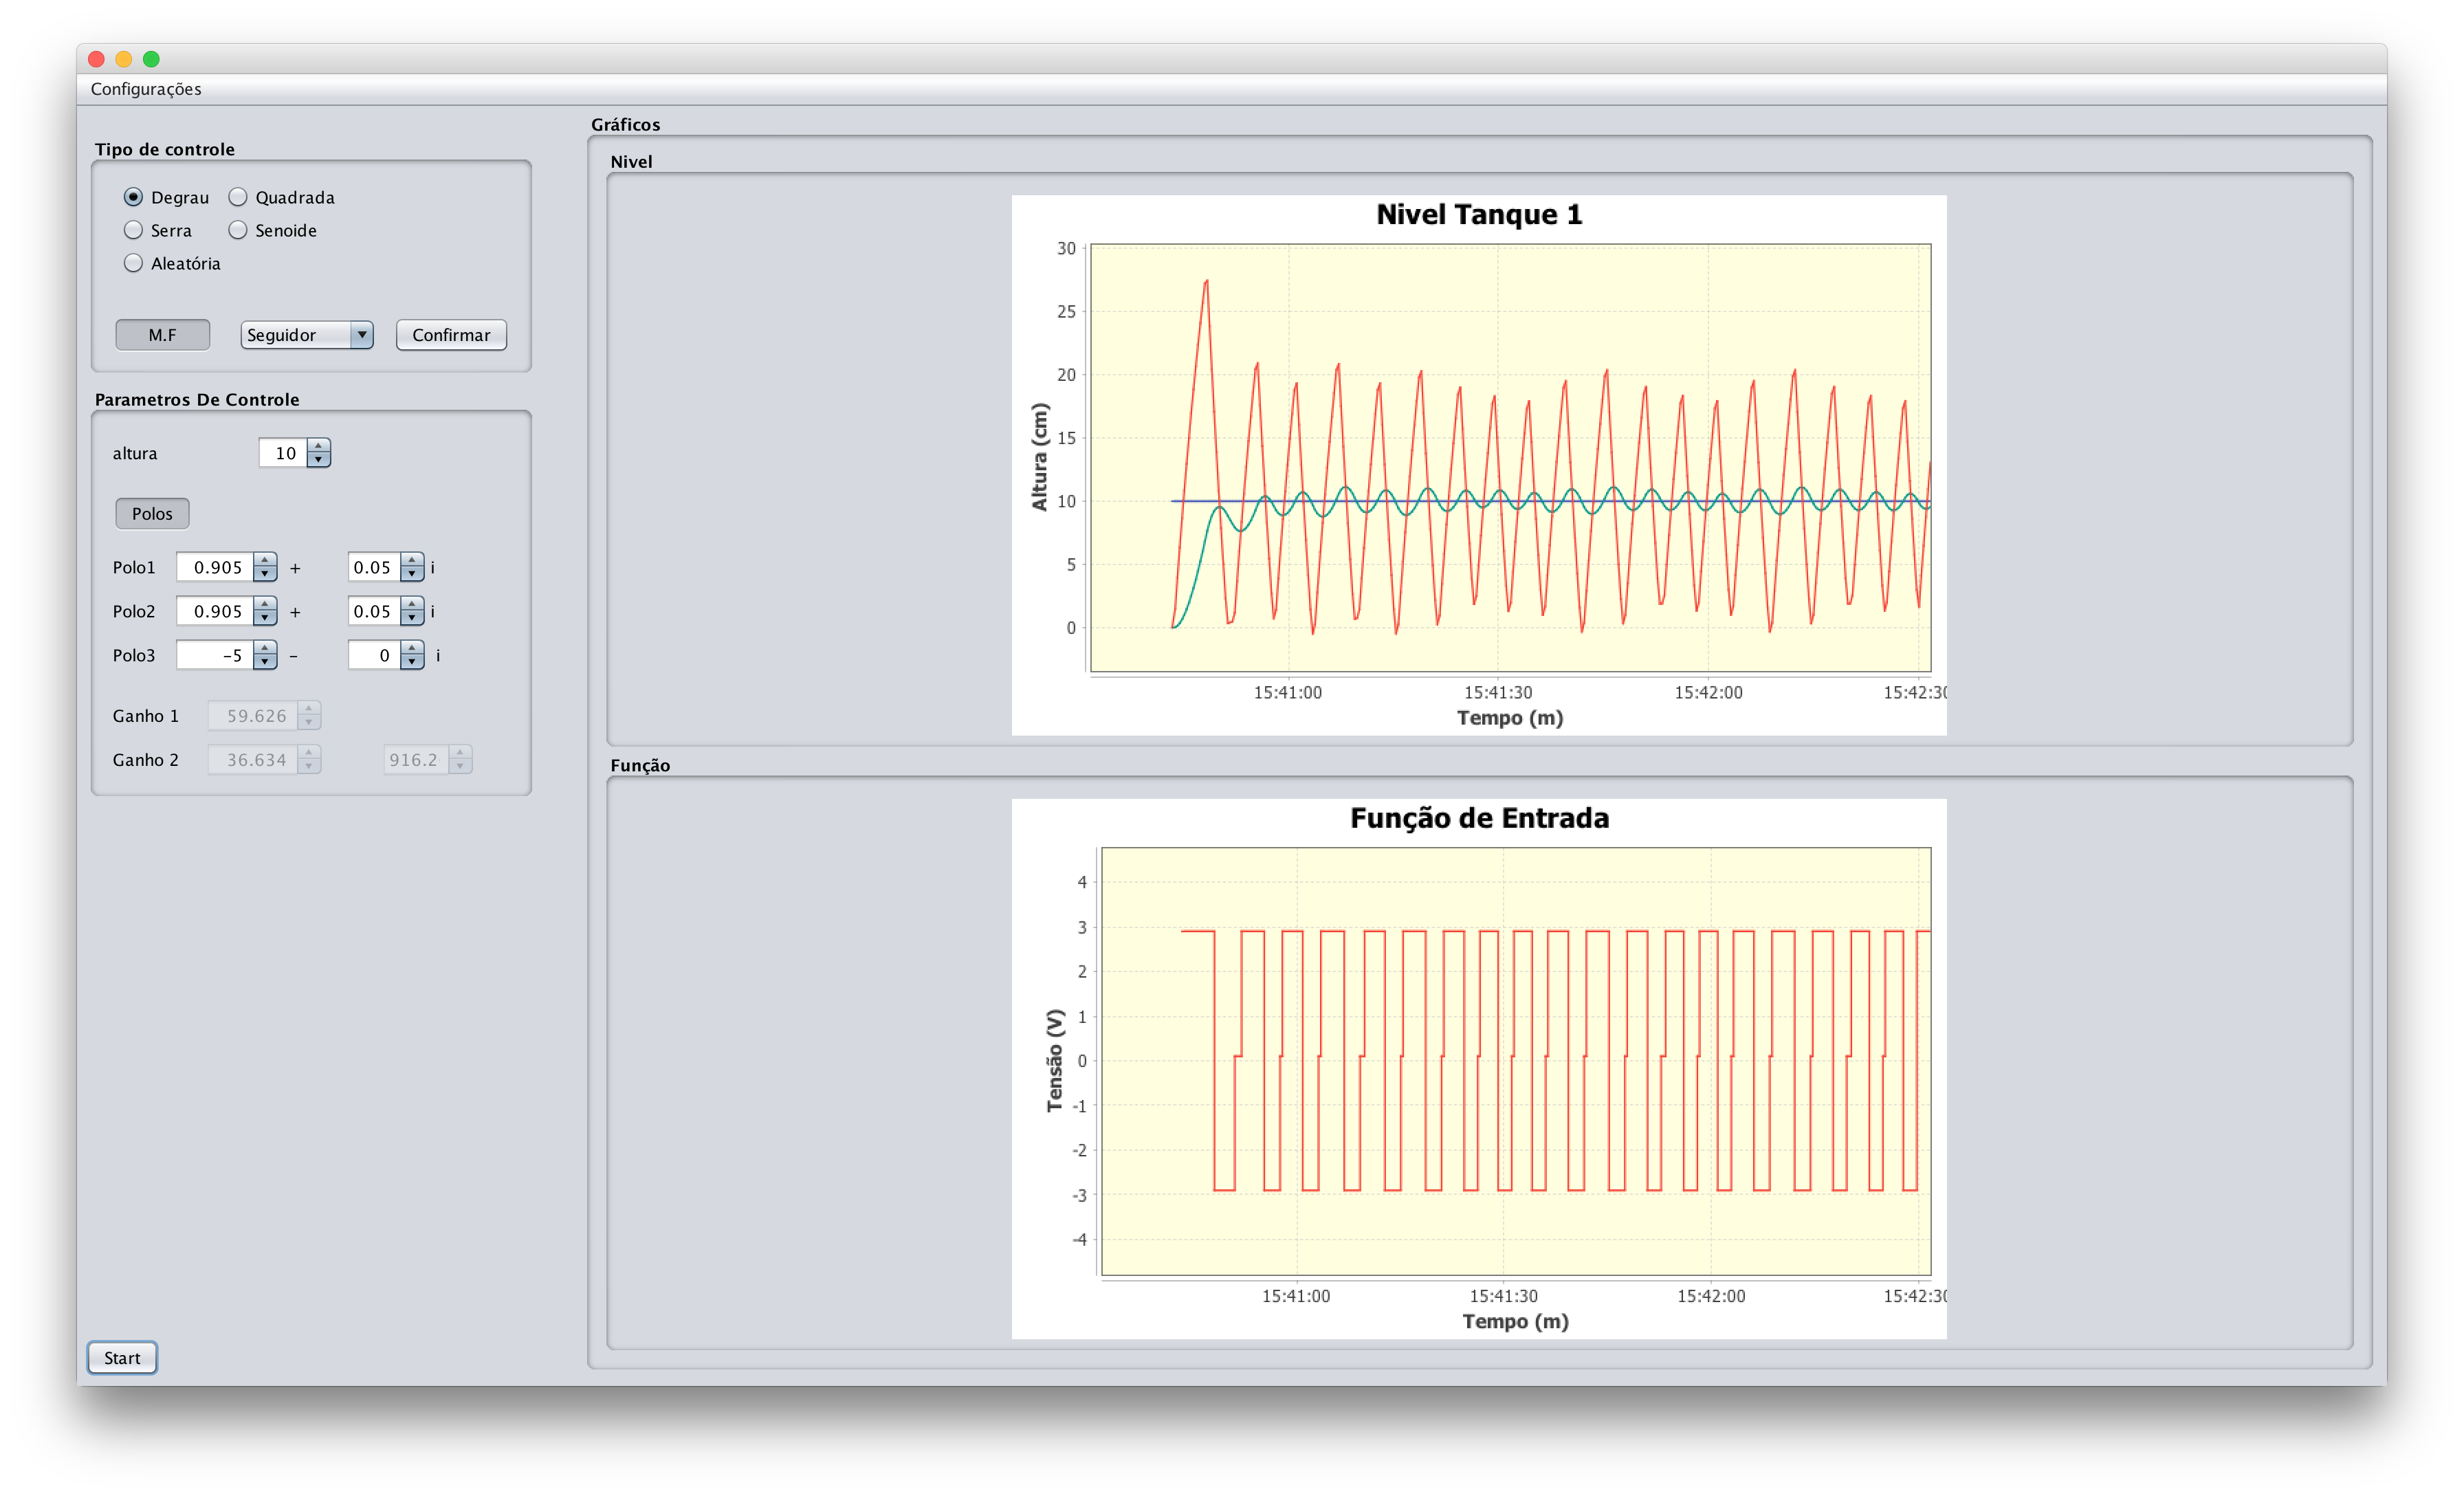
\includegraphics[scale=0.2]{Polos_0_905_i0_05__-5}
\caption{Polos: 0.905 + i0.05; 0.905 + i0.05; -5}
\end{figure}

\newpage

\thispagestyle{main}

\begin{figure}[h!]
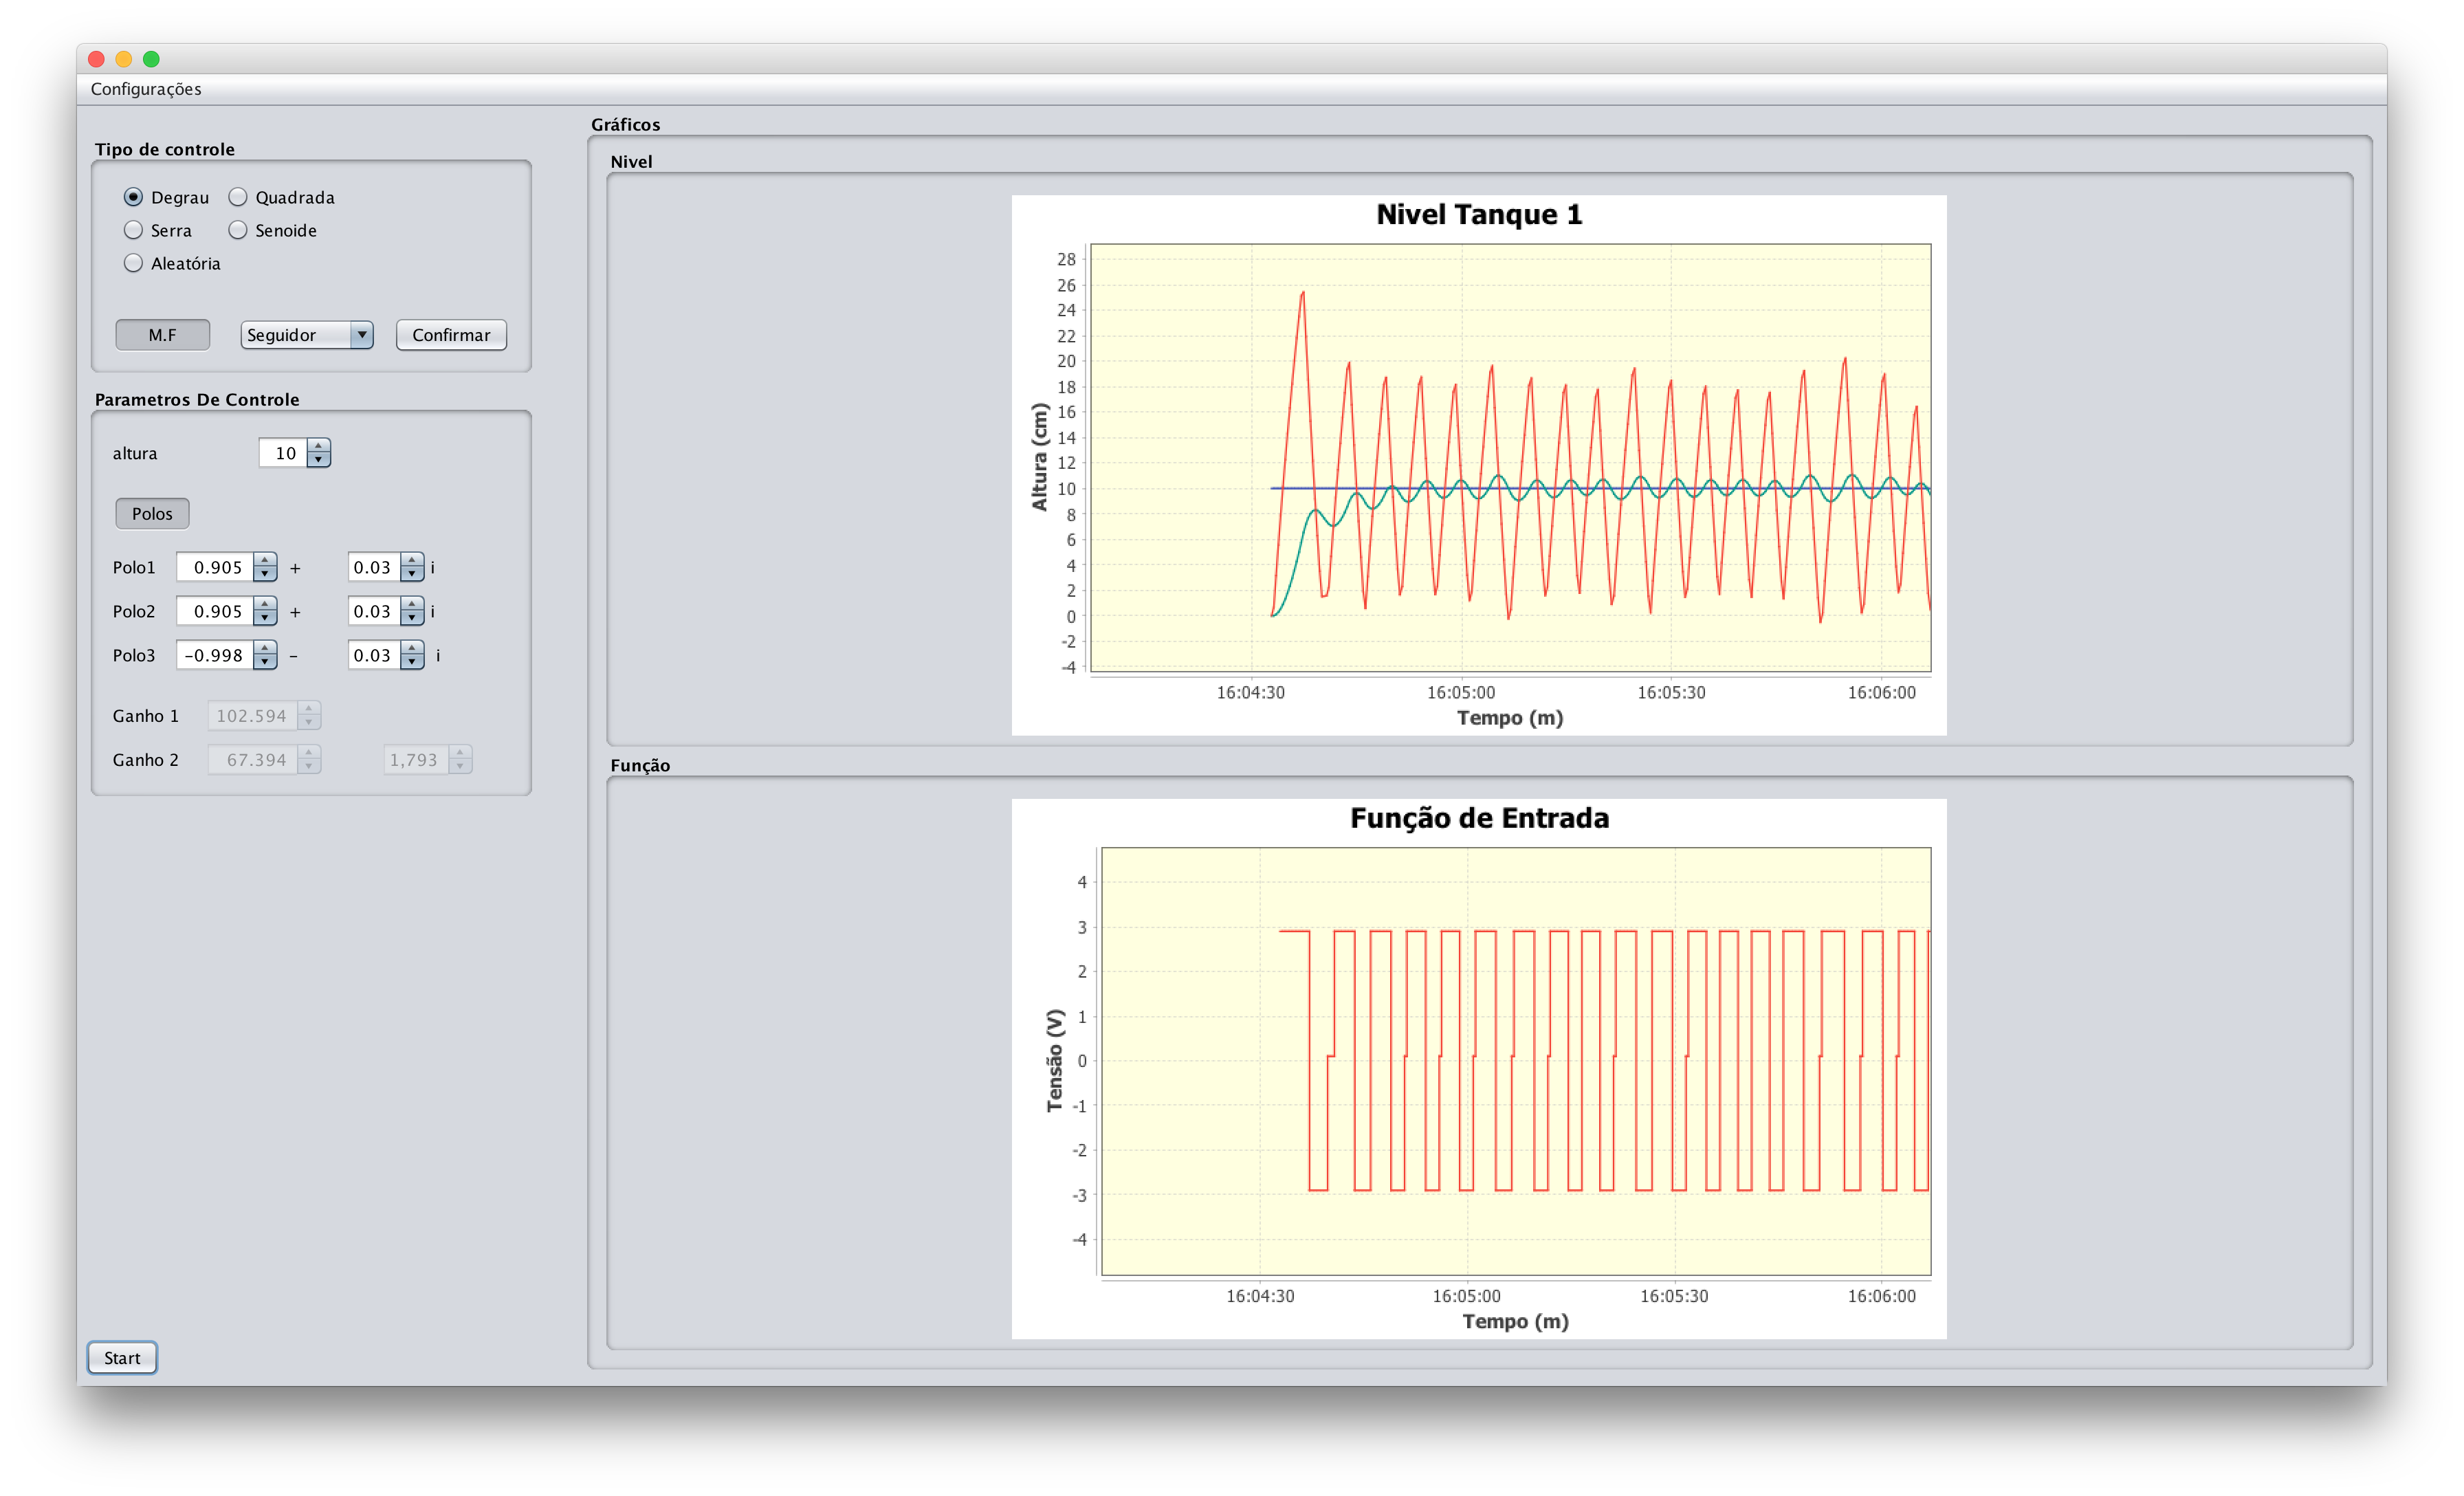
\includegraphics[scale=0.2]{Polos_0_905_i0_03__-0_998_i0_03}
\caption{Polos: 0.905 + i0.03; 0.905 + i0.03; -0.998 + i0.03}
\end{figure}

\begin{figure}[h!]
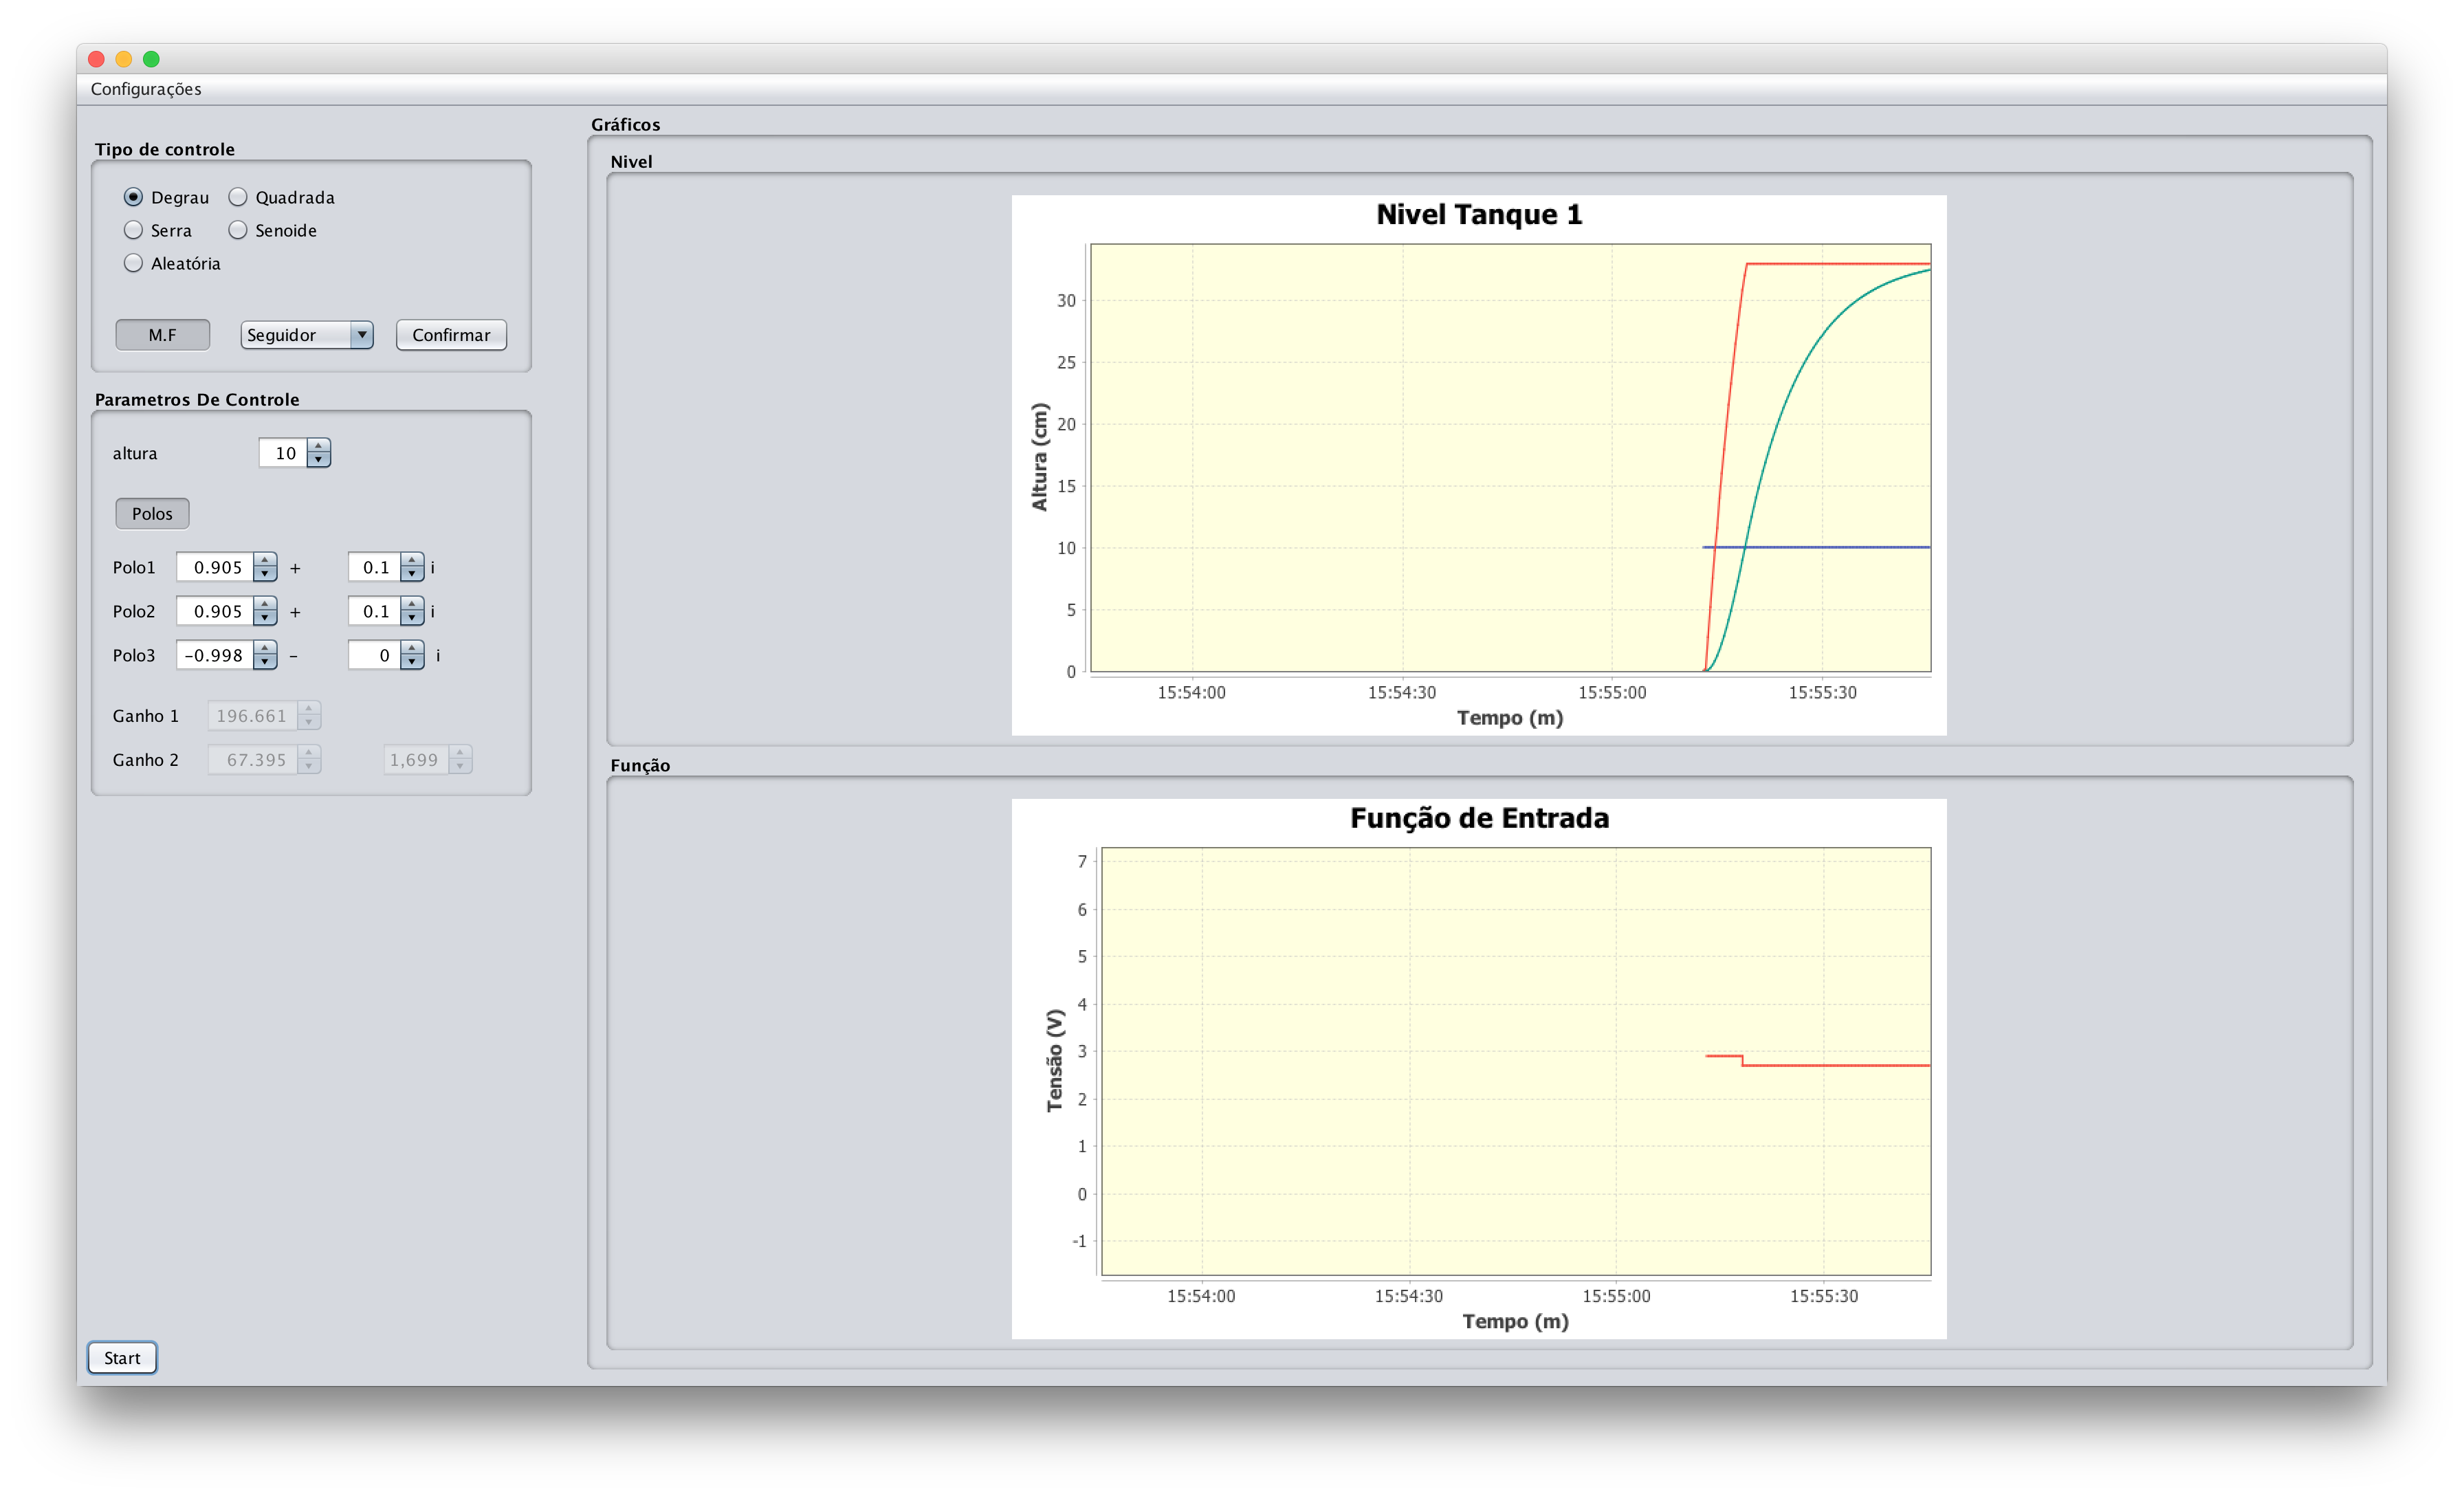
\includegraphics[scale=0.2]{Polos_0_905_i0_1__-0_998}
\caption{Polos: 0.905 + i0.1; 0.905 + i0.1; -0.998}
\end{figure}

\newpage

\thispagestyle{main}

\subsection{Ganhos}

\hspace{4ex}Com o teste dos polos do sistema, pode-se ter uma ideia do comportamento do sistema em relação aos ganhos do mesmo, na qual foram modificados e testados como mostrado nas figuras 14, 15, 16 e 17. Nesta nova abordagem, as respostas obtidas foram muito instaveis, no entanto, nos casos com ganhos em torno de 3, 90 e 2, o nívei do tanque 2 conseguiu acompanhar o set point desejado. 

\begin{figure}[h!]
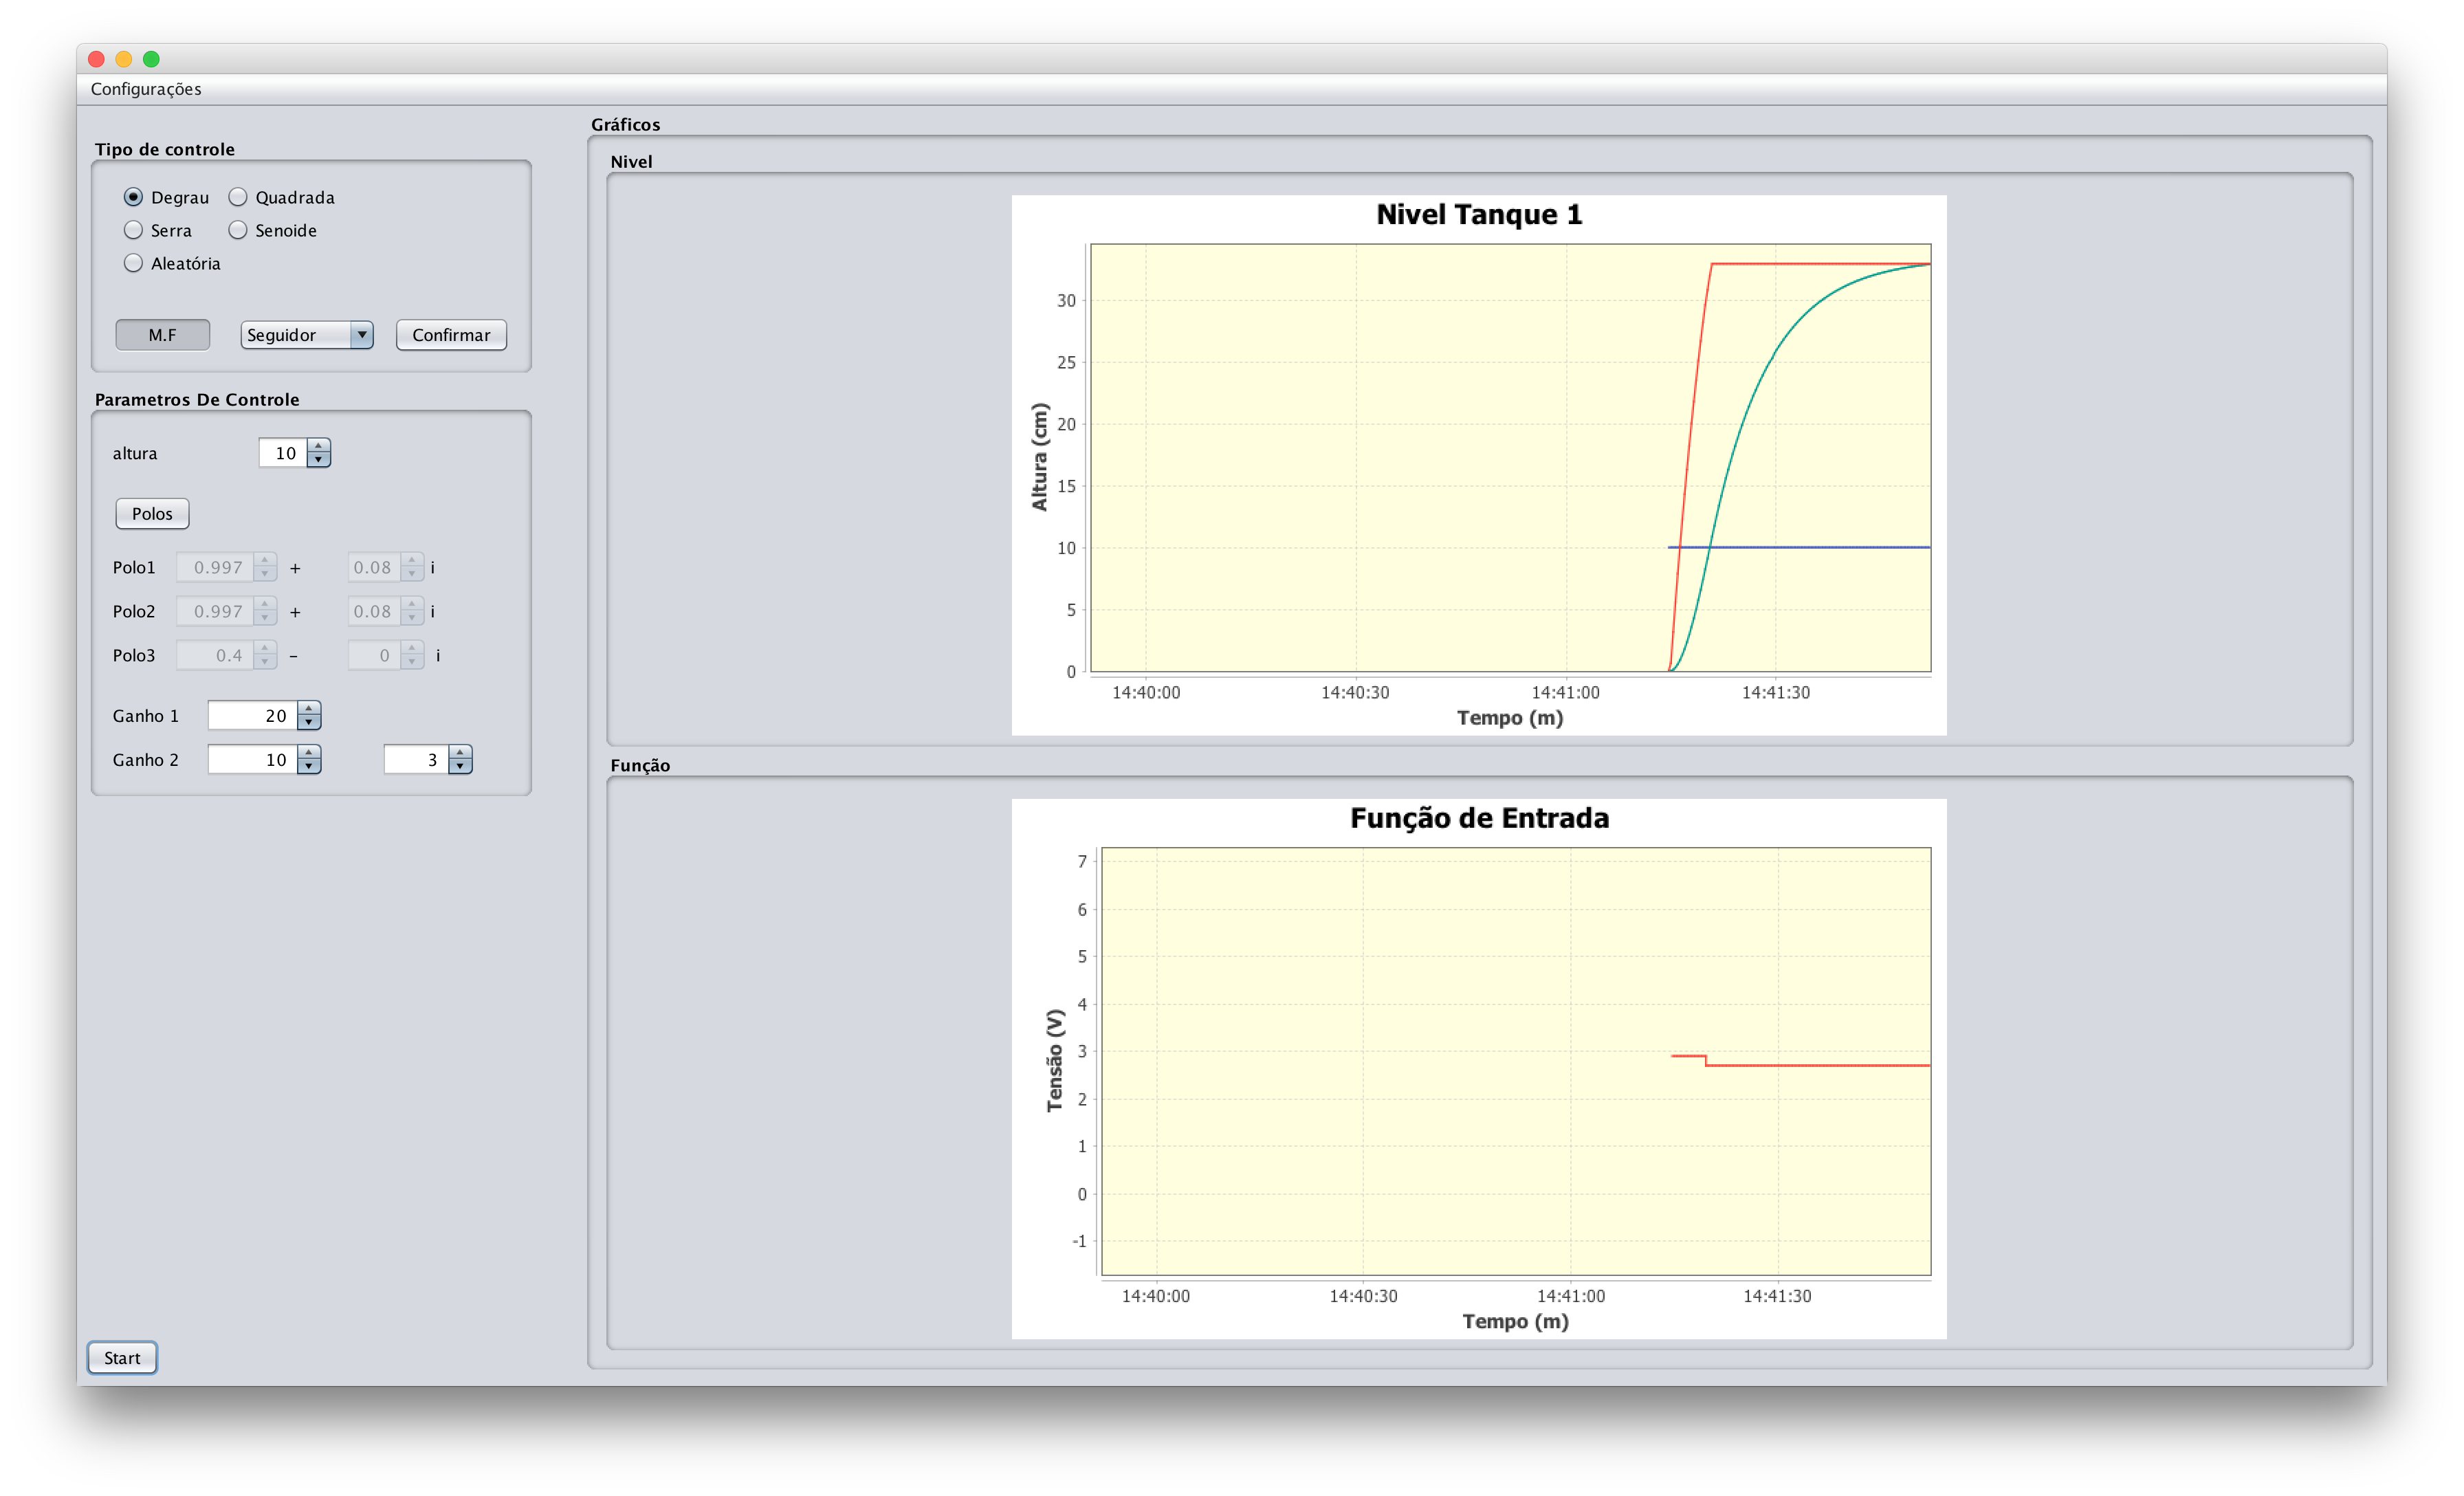
\includegraphics[scale=0.2]{Ganhos_20__10__3}
\caption{}
\end{figure}

\begin{figure}[h!]
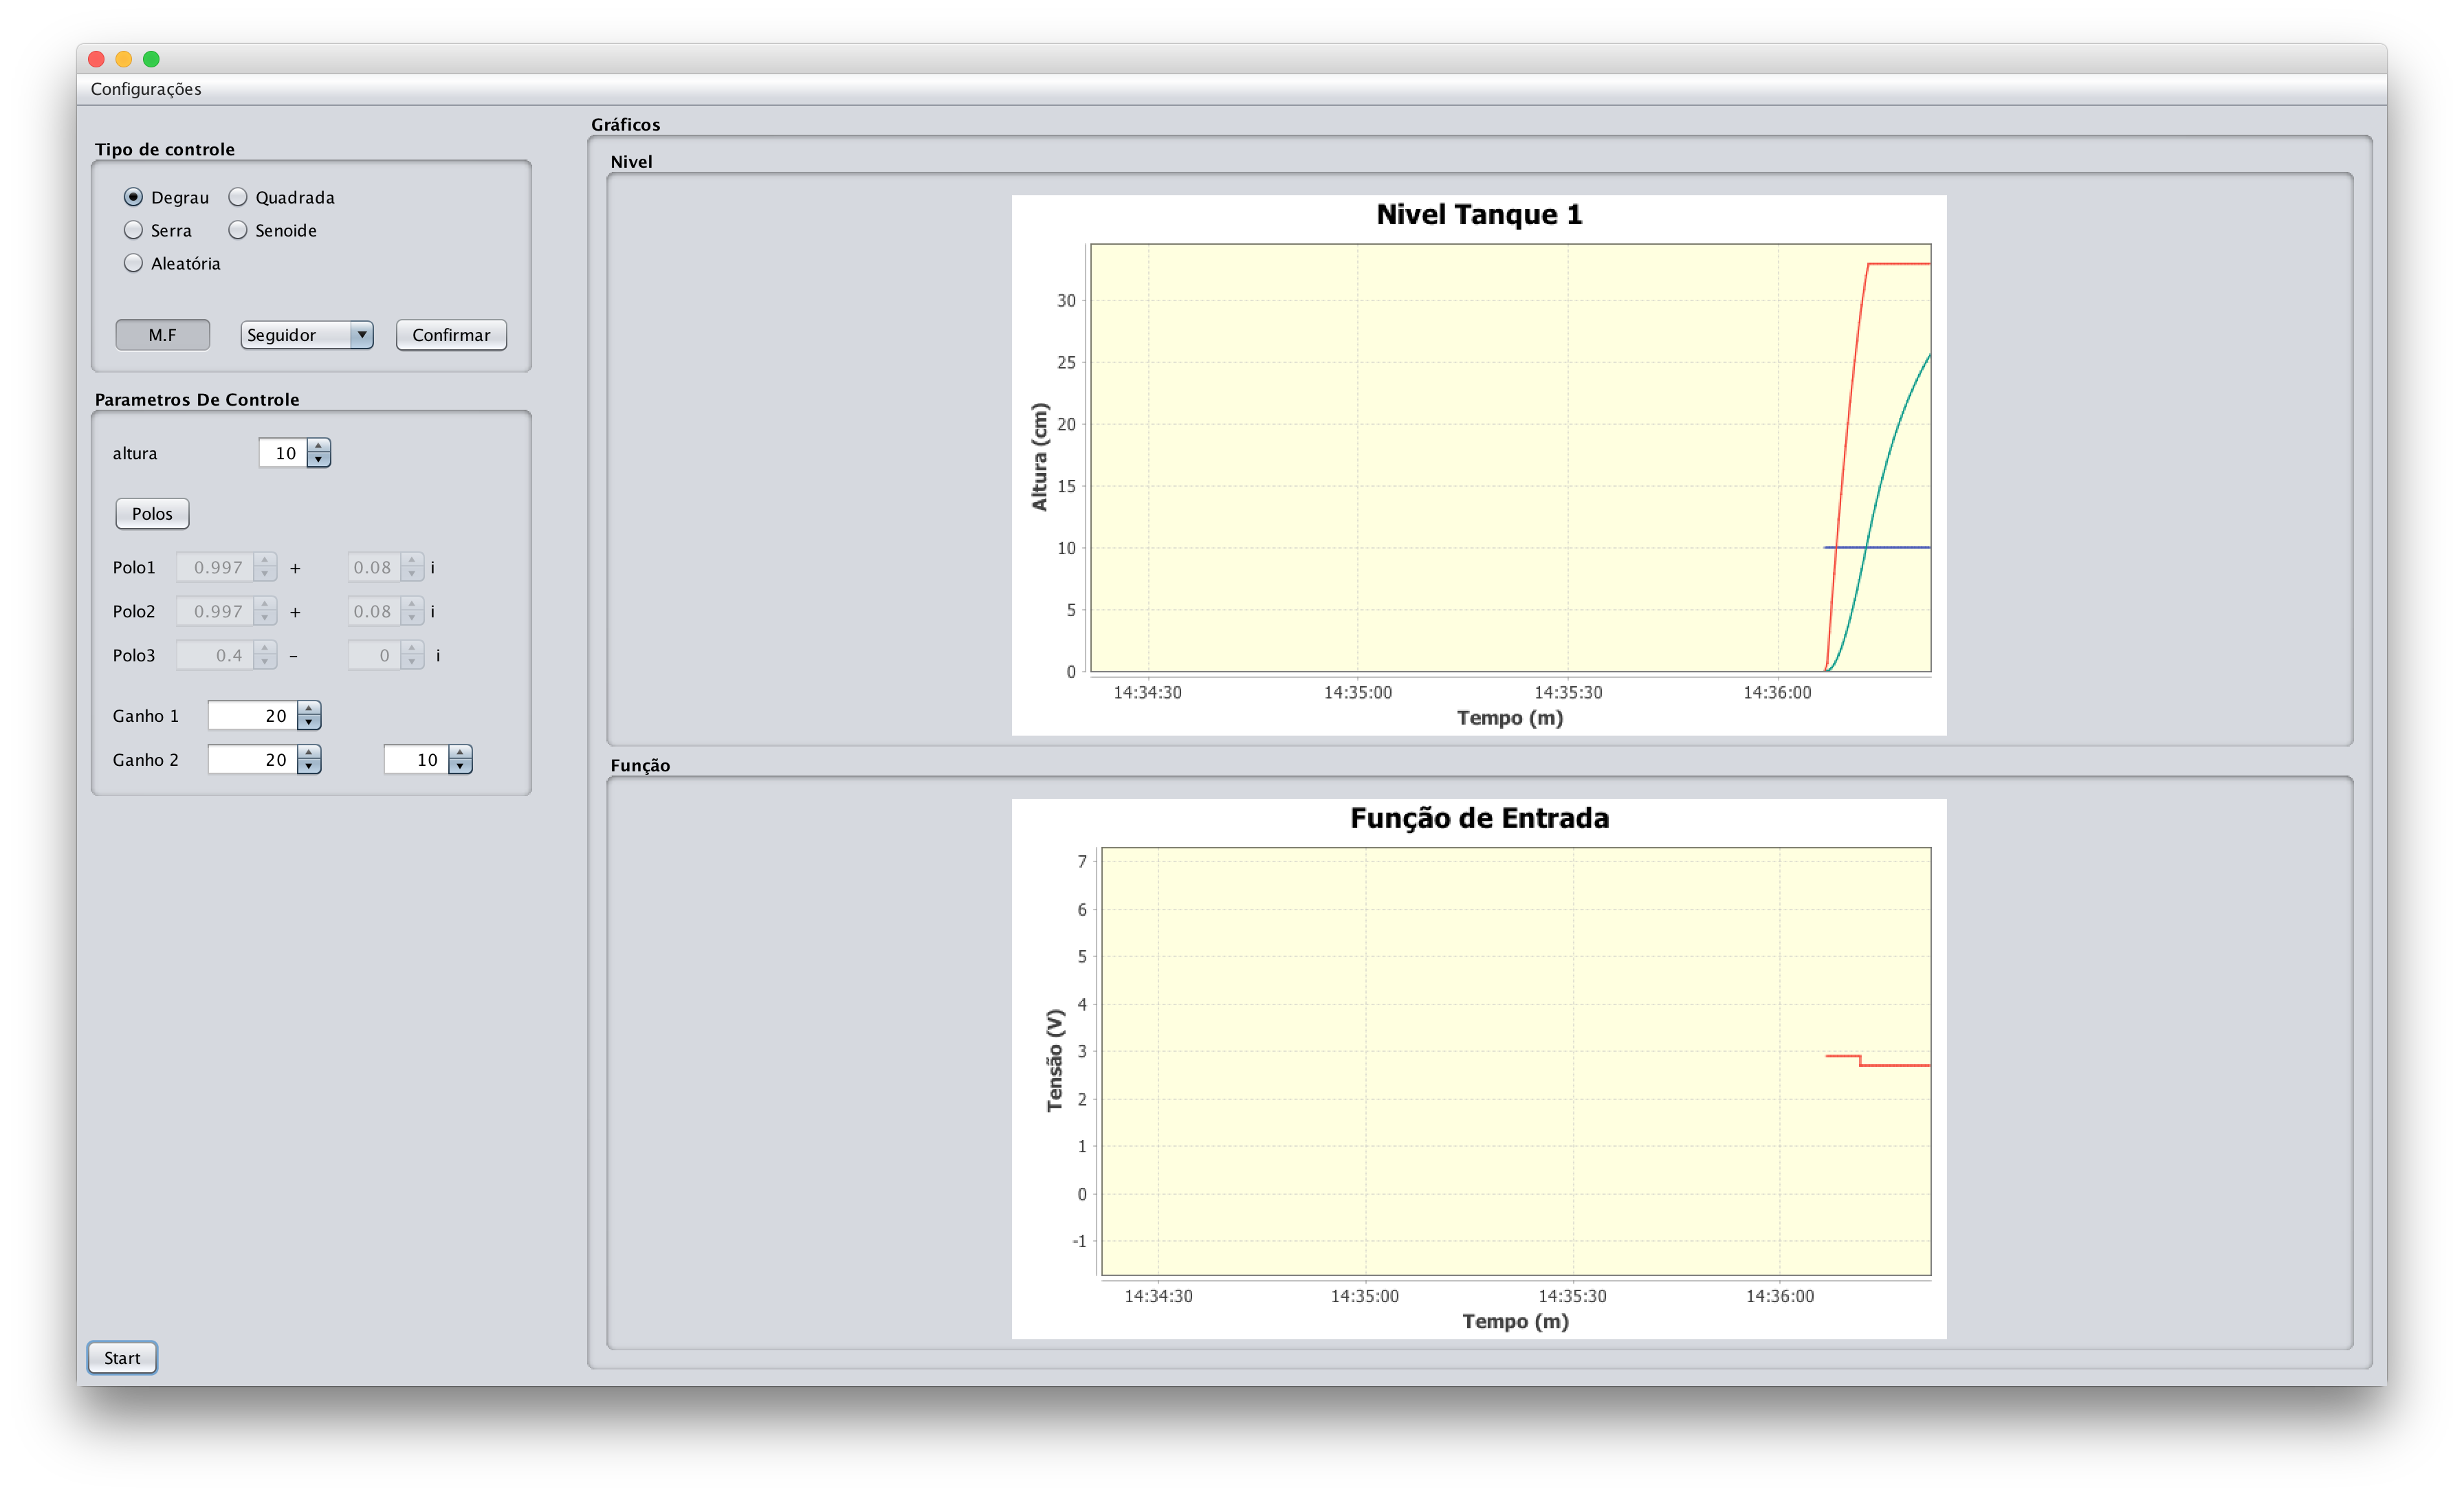
\includegraphics[scale=0.2]{Ganhos_20__20__10}
\caption{Polos: 0.905 + i0.1; 0.905 + i0.1; -0.998}
\end{figure}

\newpage

\thispagestyle{main}

\begin{figure}[h!]
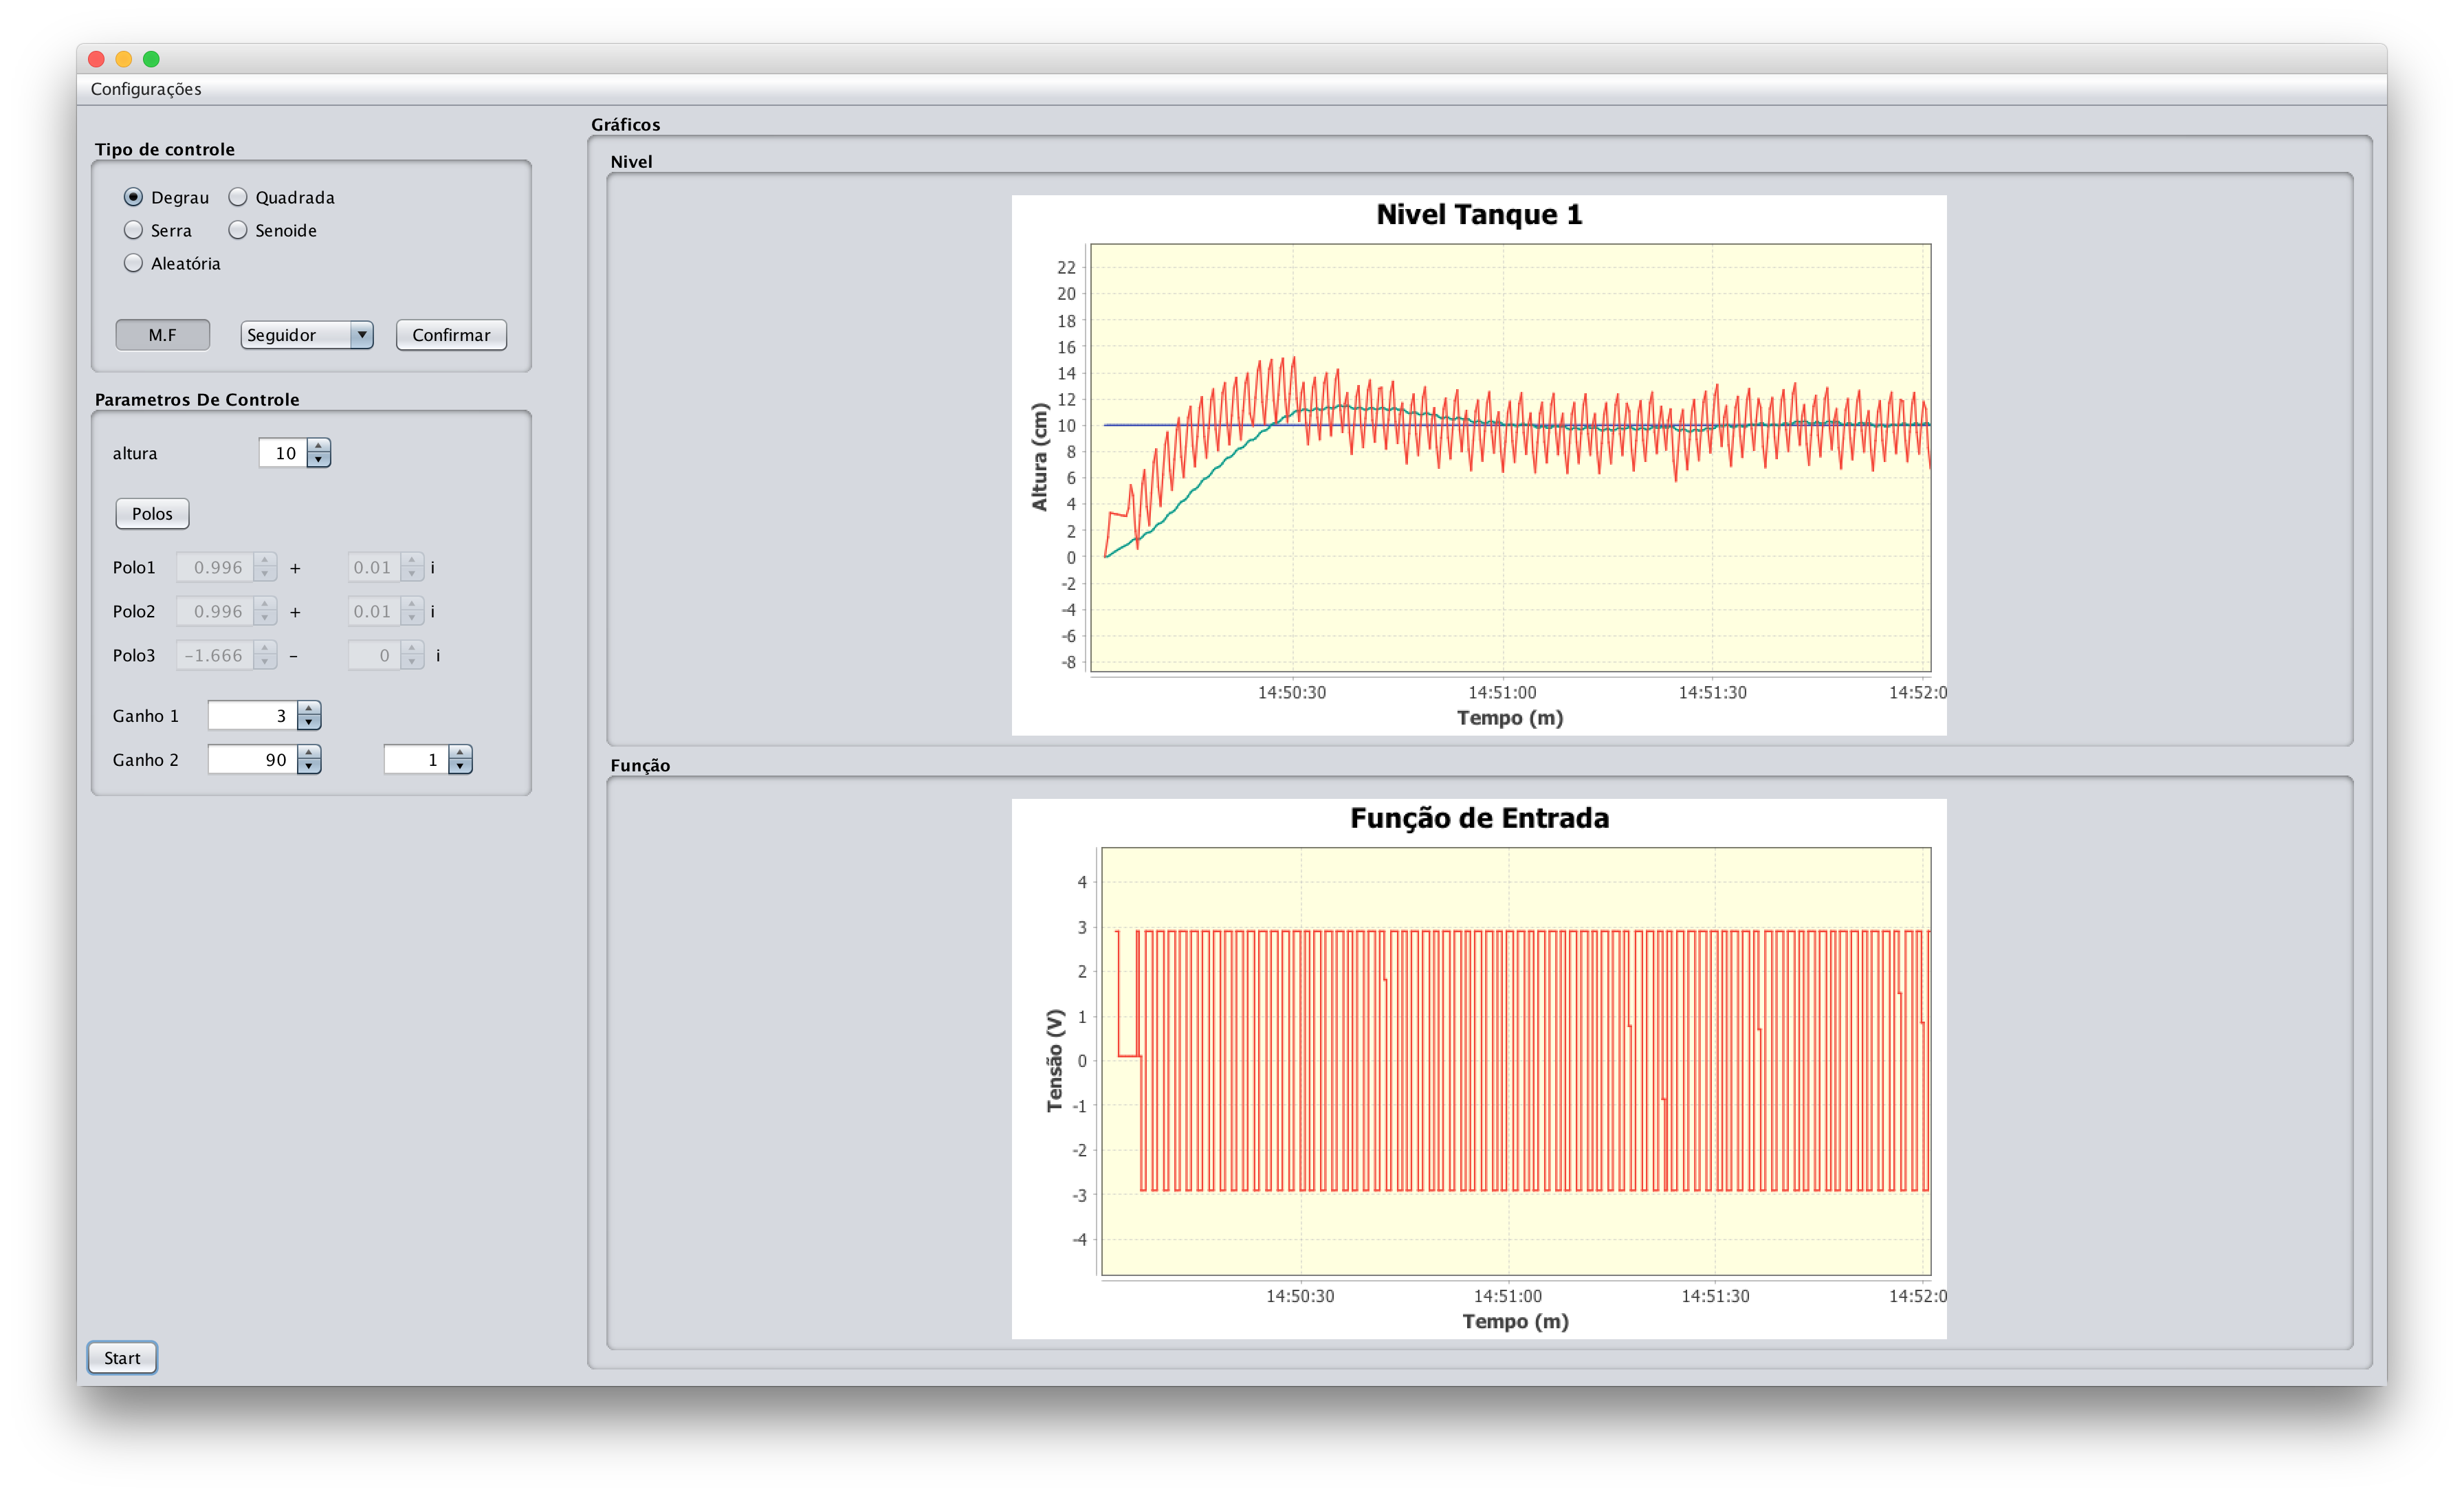
\includegraphics[scale=0.2]{Ganhos_3__90__1}
\caption{Polos: 0.905 + i0.1; 0.905 + i0.1; -0.998}
\end{figure}

\begin{figure}[h!]
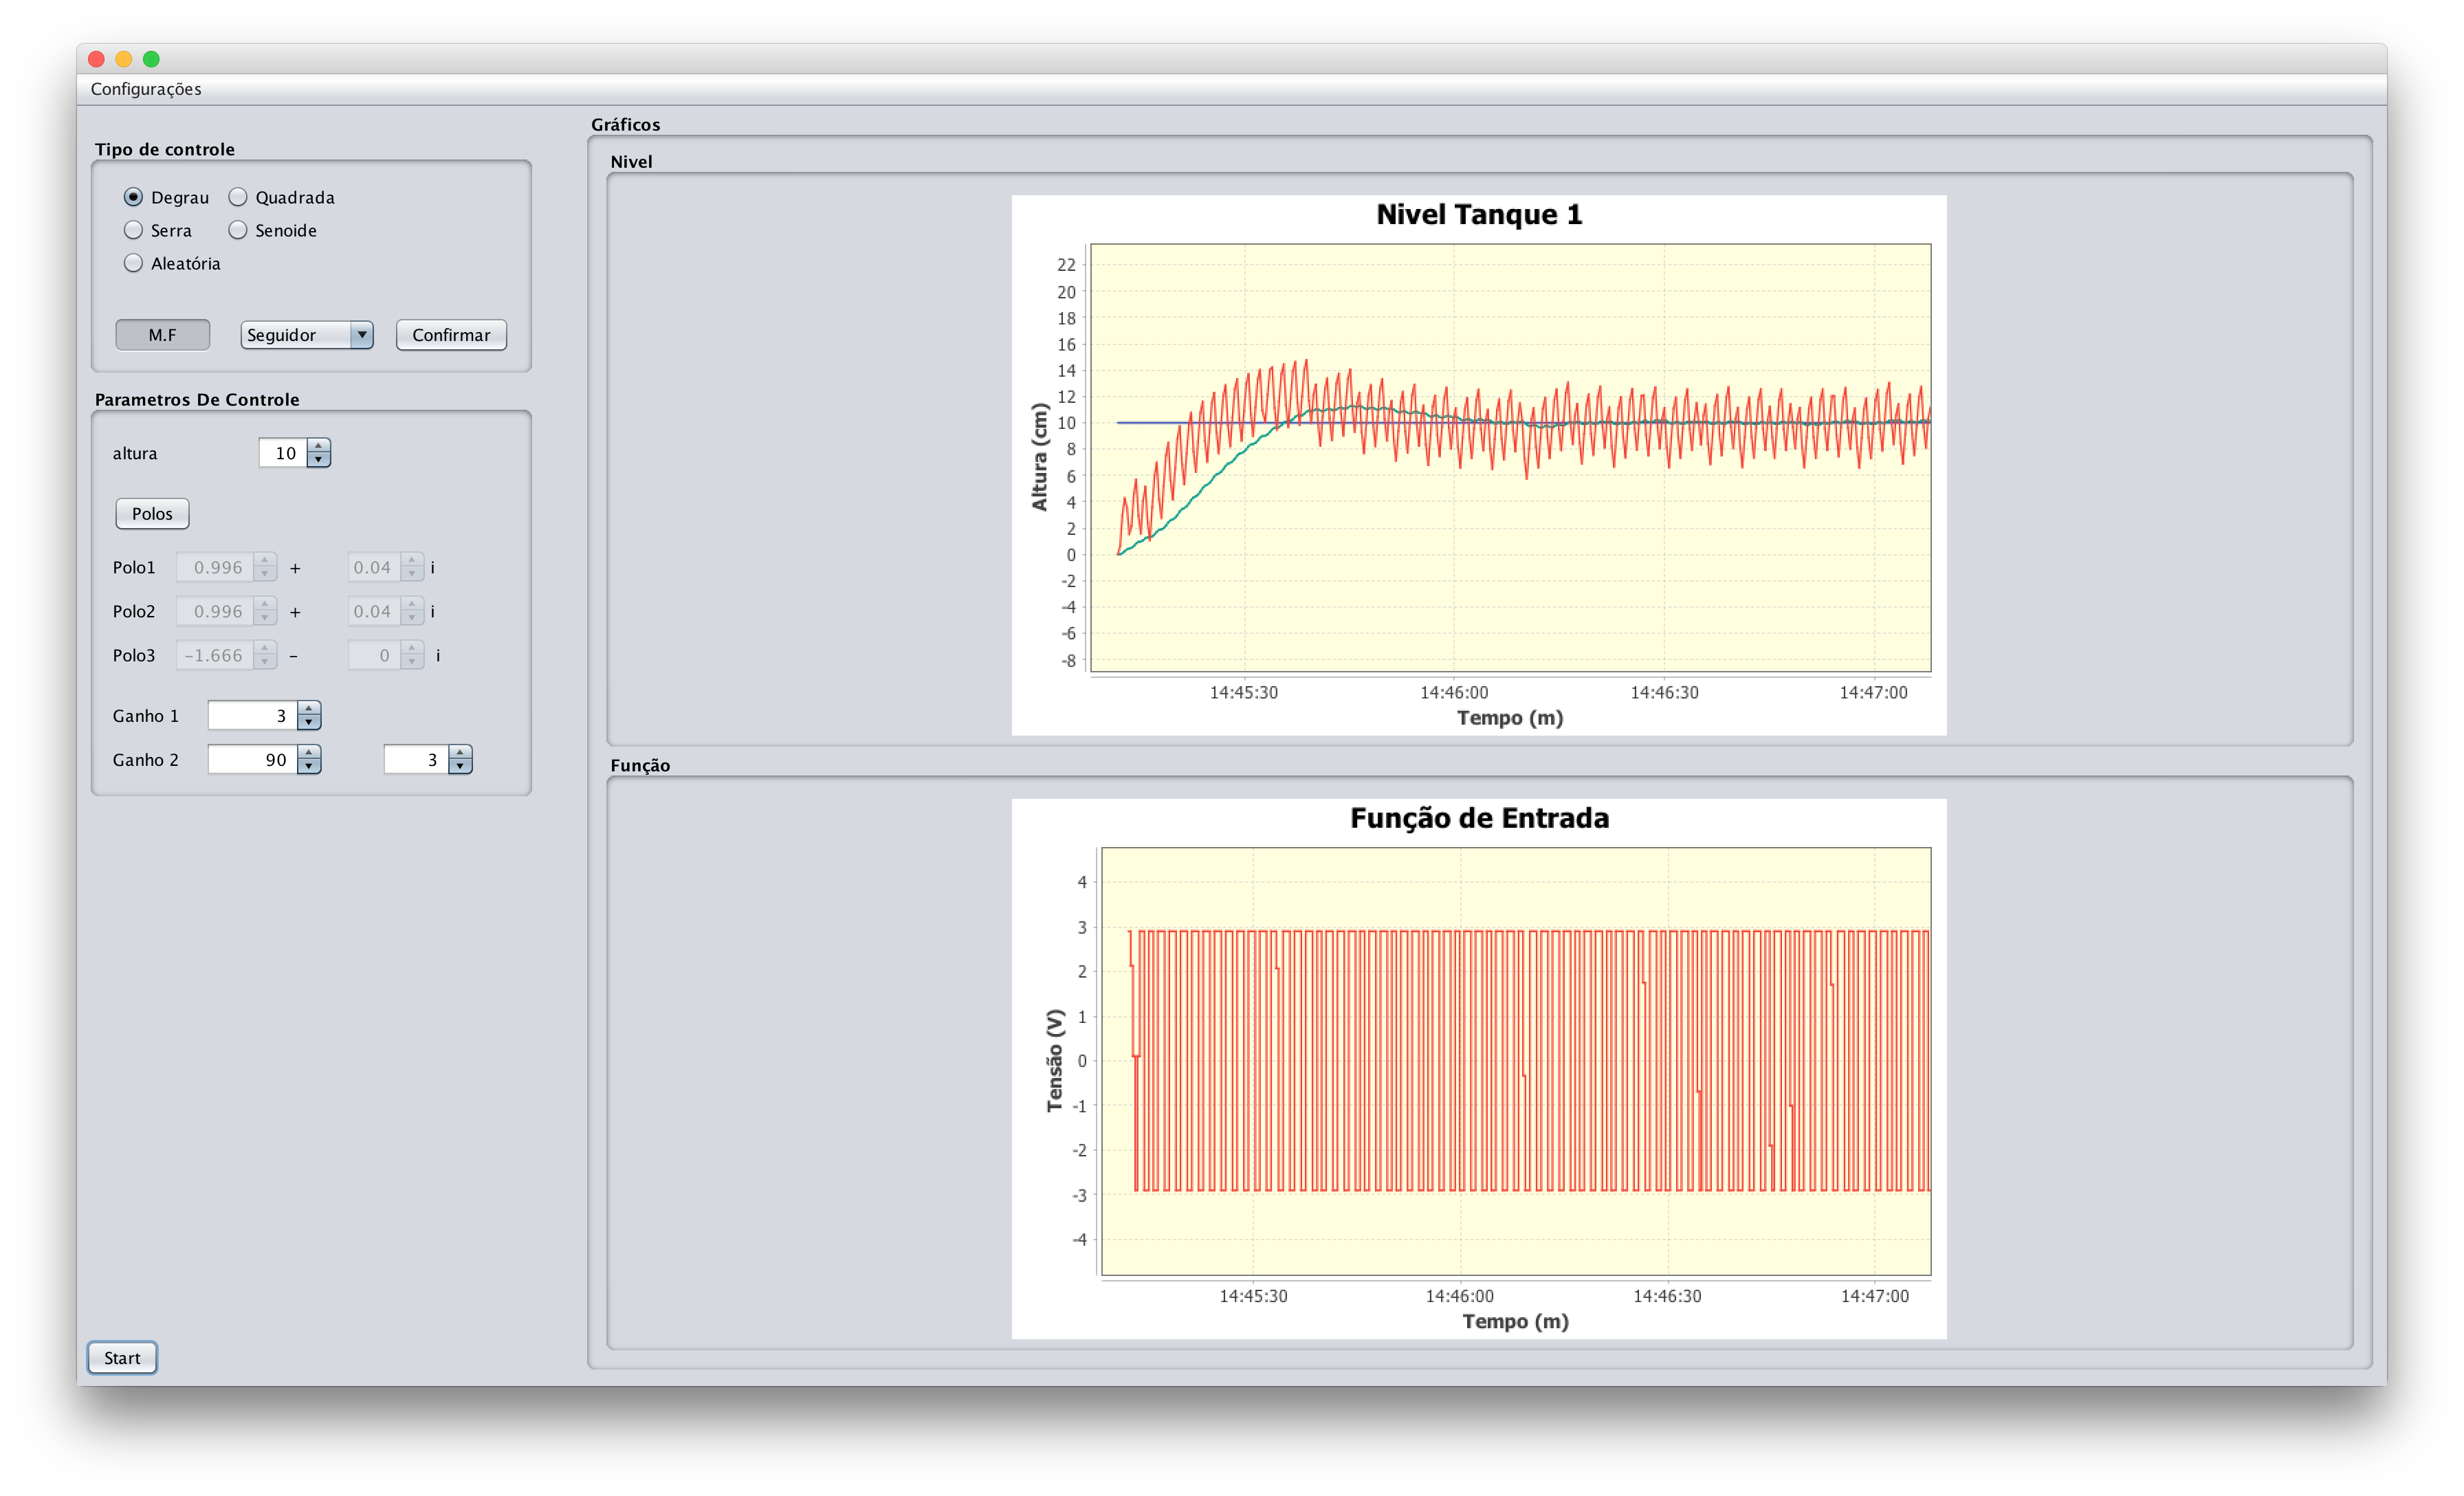
\includegraphics[scale=0.2]{Ganhos_3__90__3}
\caption{Polos: 0.905 + i0.1; 0.905 + i0.1; -0.998}
\end{figure}

\newpage

%%%%%%%%%% CONCLUSÃO %%%%%%%%%%%%%%%

\thispagestyle{main}

\section{CONCLUSÃO}


\hspace{4ex} Com o uso da aplicação implementada, atravéz dos testes realizados, foi possível ver a teoria por trás da experiência proposta. Desta forma, este trabalho nos permitiu ter uma ideia do comportamento de um sistema sendo controlado em espaço de estado com seguidor de referência.

\newpage

%%%%%%%% REFERÊNCIAS %%%%%%%%%%%%%%%%%

\thispagestyle{main}

\section{REFER\^{E}NCIAS}
% Referências bibliogáficas (geradas automaticamente)
\addcontentsline{toc}{chapter}{Referências bibliográficas}
\bibliography{bib/bibliografia}
G.F. FRANKLIN,D. POWELL e A. EMAMI-NAEINI. \textbf{Sistemas de Controle para Engenharia}. 6 \textsuperscript{a} Ed. Editora Bookman, 2013.
\appendix

%Apêndice A
\include{apendice}

\end{document}